% thesis.tex
%
% This file is root file for an example thesis written using the
% University of Wisconsin-Madison LaTeX Style file.
%
% It is provided without warranty on an AS IS basis.


%=====================================================================
% Document Style
%=====================================================================
% Choose only one of the following document classes:
%
% for a 12 Point UW PhD Thesis without Margin Check
\documentclass[12pt]{withesis}
%
% for a 10 Point UW PhD Thesis with Margin Check
%\documentclass[10pt,margincheck]{withesis}
%
% The margincheck option flags lines which overflow their hbox with a black
%  box at the end of the line.  This usually (but not always) indicates a
%  margin violation on the right margin.  Left margin violations aren't
%  indicated and if the margin violation is large enough, there isn't room
%  for the black box to be visiable.  
%
% This option can be also used in conjunction with the msthesis option.
%
% or for a 12 Point UW Masters Thesis
%\documentclass[12pt,msthesis]{withesis}
%
% or for a 10 Point UW Masters Thesis
%\documentclass[10pt,msthesis]{withesis}
%
% The msthesis option changes the page margins from 1" all around
% (the PhD format) to 1.25" left and 1" remaining margins (MS format).
% The defaults for degree and thesis are changed to be MS and thesis.
% These defaults can be overridden if the margins for the MS thesis
% are desired for other documents.

% To include optional packages, use the \usepackage command.
%  The package epsfig is used to bring in the Encapsulated PostScript
%    figures into the document.
%  The package times is used to change the fonts to Times Roman; however
%    because the times typewriter font looks odd, the original LaTeX
%    Computer Modern font is kept for the typewriter font using
%      \renewcommand{\ttdefault}{cmtt}
%    Note that Times Roman is a PostScript font and therefore, the document
%    cannot be correctly viewed from the *.dvi file.  It should be converted
%    to a *.ps file first and then viewed with a PostScript previewer...

\usepackage{geometry}
\geometry{margin=1.2in}

\usepackage[hidelinks]{hyperref}
\usepackage{url}        % Not compatible with hyperref?
\usepackage{float}
\usepackage{graphicx}
\usepackage{amsmath}
\usepackage{color}
\usepackage{times}
%\usepackage[sort]{natbib}
\usepackage{enumitem}
%\usepackage{subfigure}
\usepackage{verbatim}
\usepackage{xspace}
\usepackage{xfrac}
\usepackage{algorithmic} % must come after hyperref
\usepackage{algorithm}

\usepackage{listings}
\usepackage{microtype} %does typographical voodoo to get rid of most overfull
                       %boxes. Ideally requires pdfTeX 1.4+, going directly
                       %to pdf. Don't use a DVI workflow.
\usepackage{balance}   %\balance keywork has to be included in the last page that
                       % will not be balanced, in the first column.
\usepackage{datetime}
\usepackage{morefloats}

\usepackage{caption}
\usepackage{subcaption}
\usepackage{multirow}


\newcommand{\algrule}[1][.2pt]{\par\vskip.2\baselineskip\hrule height #1\par\vskip.2\baselineskip}
\newcommand{\eg}{{e.g.}\xspace}
\newcommand{\cf}{{cf.}\xspace}
\newcommand{\ie}{{i.e.}\xspace}
\newcommand{\etal}{{et al.}\xspace}

\newcommand{\cut}[1]{}

\renewcommand{\ttdefault}{cmtt}
\newcommand{\tightparagraph}[1]{\vspace{5pt}\noindent\textbf{#1}\ }

\newcommand{\acdc}{{AC/DC}\xspace}
%\newcommand{\acdc}{{AC/DC}\xspace}
\newcommand{\cwnd}{{{\tt CWND}}\xspace}
\newcommand{\rwnd}{{{\tt RWND}}\xspace}
\newcommand{\crs}[1]{#1}% Do nothing
\usepackage{cleveref}
\crefname{section}{§}{§§}
\Crefname{section}{§}{§§}
\crefformat{section}{§#2#1#3}
%========================================================================
%  Draft Control Commands:
%========================================================================
%
% \psdraft causes the \psfig or \epsfig commands to draw a box and label
% the box with the postscript file name instead of reading in the full
% postscript figure.  This can save time and toner when printing drafts.
%
%\psdraft
%
%
% \psfull causes the inclusion of the postscript figures.
%\psfull
%
%
%\pagestyle{thesisdraft} causes the footer text to become:
% DRAFT: Do Not Distribute        <time><Date>        <input file name>
%
%\pagestyle{thesisdraft}
%
%\pagestyle{thesis} causes the header and footers to be the correct format
%
%\pagestyle{thesis}
%
%
%  The page margins can be marked with a post-script box using the
%  \draftmargins command.  This command uses dvips's end-of-page hook
%  This is only visible in the *.ps file (NOT the *.dvi file)!
%
%\draftmargins
%
%
%  The word ``DRAFT'' can be diagonally printed across the page using
%  the \draftscreen command.  This command uses dvip's beginning-of-page
%  hook.  This is only visible in the *.ps file (NOT the *.dvi file)!
%
%\draftscreen


%=======================================================================
% Remove the following lines if appendix tables or figures are present.
% The suppress writing the auxiliary information which appears in the
% list of tables or list of figures.
%
\noappendixtables                % Don't have appendix tables
\noappendixfigures               % Don't have appendix figures


%=======================================================================
% End of Preamble, start of document
%

\lstset{basicstyle=\ttfamily,
  showstringspaces=false,
  lineskip={-2pt},
  upquote=true
%  commentstyle=\color{red},
%  keywordstyle=\color{blue}
}

\newcommand{\Name}{{PerfSight}\xspace}
\newcommand{\revise}[2]{#2}
\renewcommand{\emph}[1]{\textit{#1}}
\oralexamdate{9/29/2015}
\committeeone{Srinivasa A. Akella, Associate Professor, Computer Science}
\committeetwo{Remzi H. Arpaci-Dusseau, Professor, Computer Science}
\committeethree{Michael M. Swift, Associate Professor, Computer Science}
\committeefour{Shan Lu, Associate Professor, Computer Science, University of Chicago}
\committeefive{Xinyu Zhang, Assistant Professor, Electrical and Computer Engineering}
\date{2015}

\begin{document}

%\newgeometry{left=1in,right=1in,bottom=1in,top=1in}
% Choose your bibliography style
% plain is the basic style, others include ieeetr, siam, asm, etc
%\bibliographystyle{plain}


% prelude.tex
%   - titlepage
%   - dedication
%   - acknowledgments
%   - table of contents, list of tables and list of figures
%   - nomenclature
%   - abstract
%============================================================================


\clearpage\pagenumbering{roman}  % This makes the page numbers Roman (i, ii, etc)



% TITLE PAGE
%   - define \title{} \author{} \date{}
\title{Towards Systematic Diagnosis for Cloud Networks}
\author{Wenfei Wu}
\date{}
%   - The default degree is ``Doctor of Philosophy''
%     (unless the document style msthesis is specified
%      and then the default degree is ``Master of Science'')
%     Degree can be changed using the command \degree{}
\degree{Doctor of Philosophy}
%   - The default is dissertation, unless the document style
%     msthesis was specified in which case it becomes thesis.
%     If msthesis is specified for the MS margins, you can
%     still have a dissertation if you specify \disseration
%\disseration
%   - for a masters project report, specify \project
%\project
%   - for a preliminary report, specify \prelim
%\prelim
%   - for a masters thesis, specify \thesis
\thesis
%   - The default department is ``Electrical Engineering''
%     The department can be changed using the command \department{}
\department{Computer Sciences}
%   - once the above are defined, use \maketitle to generate the titlepage
\oralexamdate{9/29/2015}
\committeeone{Srinivasa A. Akella, Associate Professor, Computer Science}
\committeetwo{Remzi H. Arpaci-Dusseau, Professor, Computer Science}
\committeethree{Michael M. Swift, Associate Professor, Computer Science}
\committeefour{Shan Lu, Associate Professor, Computer Science, University of Chicago}
\committeefive{Xinyu Zhang, Assistant Professor, Electrical and Computer Engineering}
\date{2015}


\maketitle

% COPYRIGHT PAGE
%   - To include a copyright page use \copyrightpage
\copyrightpage

% DEDICATION
\begin{dedication}
\emph{To my parents.}
\end{dedication}

% ACKNOWLEDGMENTS
\begin{acknowledgments}

Pursuing a Ph.D. at the University of Wisconsin-Madison has been one of the most wonderful experiences of my life. I would like to take this opportunity to thank the people who guided, inspired, and accompanied me to go through this memorable experience.
 
First and foremost, I would like to thank my adviser Professor Aditya Akella. In addition to teaching me how to conduct research, his enthusiasm and focus on research set a good example for me. I am especially grateful for his support and patience during my difficulties research.
 
I would like to thank the members of my thesis committee, Remzi Arpaci-Dusseau, Michael Swift, Shan Lu, and Xinyu Zhang. Their valuable suggestions and comments greatly improved this thesis.
 
I would like to thank my mentors during my several internships, Chuanxiong GPO, Yoshio Turner, Michael Schlansker, Anees Shaikh, Guohui Wang, Alex Tessmer, and Li Erran Li. I appreciate the industrial internship 
experience I gained while working with them, particularly the chance to learn about and solve practical problems.
 
I would like to thank my fellow graduate students and postdocs, Ashok Anand, Theophuius Benson, Shan-Hsiang Shen, Aaron Gember-Jacobson, Robert Grandl, Junaid Khalid, Chaithan Prakash, David Tran-Lam, Raajay Vishwanathan, Xiaoyang Gao, Ramakrishnan Durairajan, and Brent Stephens. Working with these brilliant people is a great gift to me. I am also quite fortunate to have great friends around me, who constantly supported and cheered me: Keqiang He, Linhai Song, Yizheng Chen, Ao Ma, Yupu Zhang, Lanyue Lu, and Suli Yang.
 
Last but not least, I would like to thank my family. My parents always stand behind me with their love, support, and encouragement, and have been great sources of inspiration throughout the highs and lows of my Ph.D. work. I would also like to thank my relatives, who inspired and supported me.

\end{acknowledgments}

% CONTENTS, TABLES, FIGURES
\tableofcontents
\listoftables
\listoffigures

% NOMENCLATURE
%\begin{nomenclature}
%\begin{description}
%\item{\makebox[0.75in][l]{\TeX}}
%       \parbox[t]{5in}{a typesetting system by Donald Knuth~\cite{knuth}.  It
%       also refers to the ``plain'' format.  The proper pronounciation
%       rhymes with ``heck'' and ``peck'' and does not sound like
%       ``hex'' or ``Rex.''\\}
%
%\item{\makebox[0.75in][l]{\LaTeX}}  
%        \parbox[t]{5in}{a set of \TeX{} macros originally written by Leslie 
%        Lamport~\cite{lamport}.  The proper pronunciation is 
%        {\tt l\={a}$\cdot$tek'} and not {\tt l\={a}'$\cdot$teks} (see above).\\}
%
%\item{\makebox[0.75in][l]{{\sc Bib}\TeX}} 
%         \parbox[t]{5in}{a bibliography generation program by Oren 
%                Patashnik~\cite{lamport}
%                that can be used with either plain \TeX{} or \LaTeX{}.\\}
%
%\item{\makebox[0.75in][l]{$C_1$}} Constant 1
%
%\item{\makebox[0.75in][l]{$V$}}    Voltage 
%
%\item{\makebox[0.75in][l]{\$}}     US Dollars
%\end{description}
%\end{nomenclature}


\advisorname{Aditya Akella}
\advisortitle{Associate Professor}
% ABSTRACT
%\begin{umiabstract}
%  % abstract.tex
%
% This file has the abstract for the withesis style documentation
%
% Eric Benedict, Aug 2000
%
% It is provided without warranty on an AS IS basis.

%\noindent       % Don't indent this paragraph.
%This is not a thesis or dissertation and Master \TeX nician is not a
%degree granted at the University of Wisconsin-Madison.

%\vspace*{0.5em}
%\noindent       % Don't indent this paragraph.
%This explains the basics for using \LaTeX\ to typeset a dissertation,
%thesis or masters project or preliminary report for the University of 
%Wisconsin-Madison. Chapter
%1 talks briefly about the thesis formatting at UW-Madison.  Chapter 2 gives
%an overview of the ``essentials'' of \LaTeX{} and was written by Jon Warbrick.
%Chapter 3 talks about figures and tables and what a {\em float} is.  Chapter 4
%briefly introduces the {\sc Bib}\TeX{} program.  And finally, Chapter 5 discusses
%some of the details for using the {\tt withesis} style file.  The material in
%Chapters 2-4 basically are a review of fundamental \LaTeX{} usage and form
%a reasonable basic tutorial.%

%\vspace*{0.5em}
%\noindent       % Don't indent this paragraph.
%The style discussed in this manual was originally written by Dave Kraynie and
%edited by James Darrell McCauley as the {\tt puthesis} style for Purdue
%University's theses.  This style was modified to form the {\tt withesis} style. This
%manual is largely based on a similar manual by James Darrell McCauley and Scott Hucker.
%Permission to use, copy, modify and distribute this software and its documentation
%for any purpose and without fee is here by granted.  This software and its documentation
%is provided ``as is'' without any express or implied warranty.

Cloud outage can result in bad user experiences for cloud tenants and revenue loss to the provider. 
This makes cloud network diagnostic solutions invaluable.
Despite the various existing network diagnostic solutions, few of them are designed 
specifically for cloud networks. Current state-of-the-art cloud network diagnosis falls short 
in three aspects: (1) there is no clear way to distinguish whether an observed problem is in the 
tenant's virtual network or in the provider's infrastructure. As a result, 
the interaction between tenants and the provider leads to a longer problem-solving time 
and higher maintenance costs; (2) for cloud tenants, there are only rudimentary troubleshooting 
tools (e.g., ping, VM monitoring) that can be deployed. However, diagnosing a distributed 
system with these tools depends heavily on skill and experience, which is not always 
feasible for tenants; (3) for the cloud provider, new trends such as network function 
virtualization make the infrastructure more complex than the traditional network, 
which could lead to new problems arising. Thus, the provider requires new diagnostic tools to help
cover this range of problems.

In this thesis, we design two systems for cloud network diagnosis: (A) \emph{VND: a Virtual Network 
Diagnostic Service.} VND is a service offered by the provider to its tenants.
Using VND, a tenant can determine whether a problem is in its virtual network or not; 
VND's interfaces also simplify tenants' troubleshooting operations. A tenant could use VND to 
collect, parse and query its packet traces. Here, the trace collection cooperates within
%interface is designed in 
the tenant's view of its own virtual network without exposing the cloud infrastructure. 
Trace parse and query interfaces are design to ease the tenant's troubleshooting operations. 
VND provides a SQL interface for tenants to perform diagnosis. We show several typical 
network diagnostic use cases where troubleshooting solutions can be easily implemented using VND. 
We also measure VND's overhead and show its feasibility.
(B) \emph{PerfSight: Performance Diagnosis for Software Data Planes.}
Increasingly, modern network data planes have 
complex software involved in packet processing (e.g., virtual switches, VM hypervisors and software middleboxes).
%For example, network virtualization introduces virtual switches and VM hypervisors; network function virtualization introduces various software middleboxes. 
We refer to these software parts as the software data plane. We argue that there are at least three new
classes of performance problems that arise in software data planes: bottlenecks, contentions and bugs. 
We propose 
a system named PerfSight to target these three problems. PerfSight instruments the software 
data plane, gathers basic statistics (e.g., packet count, byte count, I/O time) and analyzes the 
statistics comprehensively. We obtained two key insights by running PerfSight: (1) packet drop is the best 
indicator of bottlenecks, and location of packet drop can give information on the resources in contention 
(e.g. CPU, network bandwidth); (2) software middlebox's states can be defined by basic statistics, 
and these states propagate in the network in certain patterns. These patterns can be used 
to infer which middlebox has performance bugs. 
%We also some case studies on how PerfSight can help with cloud management.
Our evaluation shows \Name introduces little overhead to the existing system, and thus it is 
feasible to deploy.

Together, we believe VND and \Name provide diagnostic solutions to both tenants and the provider. 
They form an integral basis for cloud network diagnosis.
%make a complement for cloud network diagnosis. 

%\end{umiabstract}

\begin{abstract}
  % abstract.tex
%
% This file has the abstract for the withesis style documentation
%
% Eric Benedict, Aug 2000
%
% It is provided without warranty on an AS IS basis.

%\noindent       % Don't indent this paragraph.
%This is not a thesis or dissertation and Master \TeX nician is not a
%degree granted at the University of Wisconsin-Madison.

%\vspace*{0.5em}
%\noindent       % Don't indent this paragraph.
%This explains the basics for using \LaTeX\ to typeset a dissertation,
%thesis or masters project or preliminary report for the University of 
%Wisconsin-Madison. Chapter
%1 talks briefly about the thesis formatting at UW-Madison.  Chapter 2 gives
%an overview of the ``essentials'' of \LaTeX{} and was written by Jon Warbrick.
%Chapter 3 talks about figures and tables and what a {\em float} is.  Chapter 4
%briefly introduces the {\sc Bib}\TeX{} program.  And finally, Chapter 5 discusses
%some of the details for using the {\tt withesis} style file.  The material in
%Chapters 2-4 basically are a review of fundamental \LaTeX{} usage and form
%a reasonable basic tutorial.%

%\vspace*{0.5em}
%\noindent       % Don't indent this paragraph.
%The style discussed in this manual was originally written by Dave Kraynie and
%edited by James Darrell McCauley as the {\tt puthesis} style for Purdue
%University's theses.  This style was modified to form the {\tt withesis} style. This
%manual is largely based on a similar manual by James Darrell McCauley and Scott Hucker.
%Permission to use, copy, modify and distribute this software and its documentation
%for any purpose and without fee is here by granted.  This software and its documentation
%is provided ``as is'' without any express or implied warranty.

Cloud outage can result in bad user experiences for cloud tenants and revenue loss to the provider. 
This makes cloud network diagnostic solutions invaluable.
Despite the various existing network diagnostic solutions, few of them are designed 
specifically for cloud networks. Current state-of-the-art cloud network diagnosis falls short 
in three aspects: (1) there is no clear way to distinguish whether an observed problem is in the 
tenant's virtual network or in the provider's infrastructure. As a result, 
the interaction between tenants and the provider leads to a longer problem-solving time 
and higher maintenance costs; (2) for cloud tenants, there are only rudimentary troubleshooting 
tools (e.g., ping, VM monitoring) that can be deployed. However, diagnosing a distributed 
system with these tools depends heavily on skill and experience, which is not always 
feasible for tenants; (3) for the cloud provider, new trends such as network function 
virtualization make the infrastructure more complex than the traditional network, 
which could lead to new problems arising. Thus, the provider requires new diagnostic tools to help
cover this range of problems.

In this thesis, we design two systems for cloud network diagnosis: (A) \emph{VND: a Virtual Network 
Diagnostic Service.} VND is a service offered by the provider to its tenants.
Using VND, a tenant can determine whether a problem is in its virtual network or not; 
VND's interfaces also simplify tenants' troubleshooting operations. A tenant could use VND to 
collect, parse and query its packet traces. Here, the trace collection cooperates within
%interface is designed in 
the tenant's view of its own virtual network without exposing the cloud infrastructure. 
Trace parse and query interfaces are design to ease the tenant's troubleshooting operations. 
VND provides a SQL interface for tenants to perform diagnosis. We show several typical 
network diagnostic use cases where troubleshooting solutions can be easily implemented using VND. 
We also measure VND's overhead and show its feasibility.
(B) \emph{PerfSight: Performance Diagnosis for Software Data Planes.}
Increasingly, modern network data planes have 
complex software involved in packet processing (e.g., virtual switches, VM hypervisors and software middleboxes).
%For example, network virtualization introduces virtual switches and VM hypervisors; network function virtualization introduces various software middleboxes. 
We refer to these software parts as the software data plane. We argue that there are at least three new
classes of performance problems that arise in software data planes: bottlenecks, contentions and bugs. 
We propose 
a system named PerfSight to target these three problems. PerfSight instruments the software 
data plane, gathers basic statistics (e.g., packet count, byte count, I/O time) and analyzes the 
statistics comprehensively. We obtained two key insights by running PerfSight: (1) packet drop is the best 
indicator of bottlenecks, and location of packet drop can give information on the resources in contention 
(e.g. CPU, network bandwidth); (2) software middlebox's states can be defined by basic statistics, 
and these states propagate in the network in certain patterns. These patterns can be used 
to infer which middlebox has performance bugs. 
%We also some case studies on how PerfSight can help with cloud management.
Our evaluation shows \Name introduces little overhead to the existing system, and thus it is 
feasible to deploy.

Together, we believe VND and \Name provide diagnostic solutions to both tenants and the provider. 
They form an integral basis for cloud network diagnosis.
%make a complement for cloud network diagnosis. 

\end{abstract}


\clearpage\pagenumbering{arabic} % This makes the page numbers Arabic (1, 2, etc)
                % Title page, abstract, table of contents, etc
\chapter{Introduction}
\label{chap:intro}
Over the past few years, cloud-based networking solutions have been gaining widespread acceptance and
deployment for organizations such as enterprises and institutions~\cite{paxson1997end}.

\section{Cloud Infrastructure Organization}
% virtual network data plane

%While our work applies to general cloud networking settings, for the purposes of 
In this thesis, we focus on multi-tenant cloud data centers.
In this setting, tenants deploy \emph{virtual private clusters}
composed of application end-points (this could be service software in

\section{Challenges in Diagnosing Cloud Networks}
\label{sec:intro:challenges}
Troubleshooting network problems is difficult. A network is a distributed

\begin{itemize}
\item Cloud networks have higher complexity than traditional networks.  In data planes, network virtualization introduces more software components, including software switches, hypervisors, and so on; software middleboxes are introduced to support network function virtualization. In control planes, the cloud controllers need to perform more functions to set up virtual networks; the controllers map tenants' requirements from a logical view to a physical view, and finally to devices rules. Cloud networks involve a greater number of components involved, and these components may have logical or physical dependency (e.g., exchanging data or sharing hardware resources). This complexity in cloud networks makes them not only more error-prone but also difficulty to manage and diagnose.
\item The two roles in cloud networks makes the management trickier than traditional network. The two roles are the provider (or operator) and the tenants, and their information is isolated from each
other. In the case of network problems, the interaction between the provider and
the tenants is crucial for problem solving; however, this process is usually of low efficiency. 
The tenants observe misbehaviors of their applications directly, but they lack diagnostic tools.
The provider does not know the applications' performance, so they can only wait for tenants' tickets.
%Due to the isolation, both parties cannot perform a complete diagnosis; therefore, 
The two parties need to exchange observations to figure out the problem. This manual process increases
the problem-solving time and maintenance cost.
\item The visibility of cloud networks is not well provided to customers and operators. In traditional networks, network devices and components provide various information for operators to monitor or troubleshoot, e.g., packet drop statistics in switches and the network protocol stack. However, by our study, this kind of visibility is not well preserved in cloud networks. For customers, the cloud provider does not provide visibility of how their packets traverse the network for security reasons. For the provider, some virtualization components are introduced to cloud networks without keeping the visibility for diagnosis\textemdash there are several silent packet drops in VM hypervisors and software middleboxes. This is partially due to the fact that developers typically focus on functionality instead of diagnostic features in the first few versions of the software.
\end{itemize}


\section{An Overview of Our Approach}
\label{sec:intro:approach}
Ever since the birth of networks, network problems have been appearing and upseting network operators. There have been numerous proposals aiming to solve various problems. For example, there are standards or technologies such as SNMP, sFlow, and NetFlow to collect states in networks; there are network models and diagnostic algorithms to discover culprits in network problems; and there are various network diagnostic solutions for traditional networks and software-defined networks, which combine the technologies and algorithms. These approaches are undoubtedly valuable in their specific scenarios.

However, these solutions do not overcome the challenges in diagnosing cloud networks (Section~\ref{sec:intro:challenges}). In this thesis, we make a study of problems in cloud networks. According to the cloud organization, we look into each planes and summarize new problems. In more details, we found that in application planes, the isolation between tenants and the provider causes tenants unable to diagnose their virtual networks, thus we propose, design and implement a virtual network diagnostic service in application planes. We found that in data planes, increasing complexity and lack of visibility cause performance problems difficult to be identified, thus we modify software data planes, collect statistics and leverage the statistics to perform accurate diagnosis. We also find inconsistency issues in control planes, where tenant requirements may not be consistency with physical device states; we leave this problem in future works.

Decomposing cloud networks into three planes and reconsidering diagnostic challenges in cloud networks is an efficient way to discover, abstract and solve cloud network problems. We feel that, owing to our approach, several cloud-specific problems are discovered. Therefore, our works improve the reliability of cloud networks.

\section{Thesis Outline}
\label{sec:intro:outline}
The rest of this thesis is organized as follows. 
In Chapter~\ref{chap:background}, we make a study of cloud network problems and briefly describe our approaches.
In Chapter~\ref{chap:vnd},
we describe our design of the virtual network diagnostic service. In Chapter~\ref{chap:perfsight},
we present our solution for software data plane diagnosis.
In Chapter~\ref{chap:related}, we discuss the related work, 
Finally in Chapter~\ref{chap:conc}, we conclude this thesis and discuss options for future work.
                  % Chapter 1
%\section{Design Decisions and Challenges}
\label{sec:background}

In Presto, we make several design choices to 
build a highly robust and scalable system that provides near optimal load 
balancing without requiring changes to the transport layer or switch hardware. We 
now discuss our design decisions.


\subsection{Design Decisions}

\tightparagraph{Load Balancing in the Soft Edge} A key design decision in Presto 
is to implement the functionality in the soft edge (\ie{}the vSwitch and hypervisor) of 
the network. 
%should we motivate why not to do it in hardware?
%A current trend in datacenter design is to utilize network equipment from 
%original design manufacturers (ODMs) in order to simplify and customize
%the network. This has been reported to significantly reduce costs and improve
%network performance~\cite{aws-peek}.
%Motivation here is that network is becoming very simple, and functionalities
%are being moved to an intelligent edge. Examples are VMWare/NSDI, Fabric, NFV in vSwitch,
%SDNs/OpenFlow, 
% Given recent advancements in this space\eric{what advancements? can we be more specific
% in order to provide better motivation?}, we believe the soft edge is the best 
% place to deploy new network functions, such as load balancing, in a scalable and 
% distributed manner.\eric{is this a new position? vmware nsdi paper...}
The vSwitch occupies a unique position in the networking stack 
in that it can easily modify packets without requiring any changes to customer VMs or transport layers.
Functionality built into the vSwitch can be made aware of the underlying hardware offload
features presented by the NIC and OS, meaning it can be fast.
Furthermore, an open, software-based approach prevents extra hardware cost and vendor 
lock-in, and allows for simplified network management. 
These criteria are important for providers today~\cite{aws-peek}.
Thanks to projects like Open vSwitch, 
soft-switching platforms are now fast, mature, open source, adopted widely, remotely 
configurable, SDN-enabled, and feature-rich~\cite{ovs-edge,nv-mtd,pfaff2015design}. Presto is built on these 
platforms.

\tightparagraph{Reactive vs Proactive Load Balancing} The second major design decision in 
Presto is to use a proactive approach to congestion management. Bursty 
behavior can create transient congestion that must be reacted to 
before switch buffers overflow to prevent loss (timescales range from 100s of $\mu$s 
to around 4 ms~\cite{planck}). This requirement renders most of the centralized reactive schemes ineffective
as they are often too slow to react to any but the largest network events,~\eg{}link failures. 
%Not reacting to transient congestion can increase tail latencies.
Furthermore, centralized schemes can hurt performance when rerouting
flows using stale information.
%By reacting on a different scale than the congestion, centralized schemes may reroute flows
%on stale information, which can hurt performance.
Distributed reactive schemes like MPTCP~\cite{mptcp} and 
CONGA~\cite{conga} can respond to congestion at faster timescales, but have a high barrier to deployment.
Furthermore, distributed reactive schemes must take great care to avoid oscillations.
Presto takes a proactive, correct-by-design approach to congestion management. 
That is, if small, near-uniform portions of traffic are equally
balanced over a symmetric network topology, then the load-balancing can remain agnostic to congestion and
leave congestion control to the higher layers of the networking stack.
%then we don't need to 
%be reactive to congestion.
Presto is only reactive to network events such as link failures. Fortunately, 
the larger timescales of reactive feedback loops are sufficient in these scenarios. 

\tightparagraph{Load Balancing Granularity} ECMP has been shown to be ineffective at load balancing the network, and thus many schemes advocate load balancing at a finer granularity than a flow~\cite{drb,conga,juniper-vcf,packetspray}. A key factor impacting the choice of granularity is operating at high speed. 
%and ensuring suitable application level performance.
%Implementing fine-grained, near-uniform load balancing in 10+ Gbps networks
%is difficult.
Operating at 10+ Gbps incurs great computational overhead, and therefore host-based load balancing schemes
must be fast, light-weight and take advantage of optimizations provided in the networking stack.
For example, per-packet load balancing techniques~\cite{drb} cannot be
employed at the network edge because TSO does not work on a per-packet
basis. TSO, commonly supported in OSes and NICs, allows for large TCP segments (typically 64 KB in size)
to be passed down the networking stack to the NIC. The NIC breaks the segments into MTU-sized packets and copies and computes
header data, such as sequence numbers and checksums. When TSO is disabled, a host incurs 100\% utilization of one CPU core and can only achieve
around 5.5 Gbps~\cite{bullettrains}. Therefore, per-packet schemes are unlikely to scale to fast networks without hardware support.
Limiting overhead by increasing the MTU is difficult because
VMs, switches, and routers must all be configured appropriately, and traffic
leaving the datacenter must use normal 1500 byte packets. Furthermore, per-packet schemes~\cite{drb,packetspray} are likely to
introduce significant reordering into the network.
%Achieving line rate at 10 Gbps is nontrivial because dealing
%with so many 1500 byte MTU-sized packets at varying layers
%of the networking stack causes significant computational overhead.
%Therefore, modern operating systems and network adapters have many
%optimizations to help burden the load.
%On the sender side, TCP Segmentation Offload (TSO)~\footnote{Generically known as large segment offload or generic segmentation offload}
%is designed to allow the TCP/IP stack to deal with large TCP segments. Segments, up to 64 KB in size, are passed
%from the application layer all the way down to the NIC, which in turn breaks the large segment down into 1500 byte packets.
%The NIC copies and calculates the header information, such as checksums and sequence numbers.
%This allows the computational burden to be substainally lessened, and therefore rates of 10+
%Gbps can be achieved. With TSO disabled, achievable 10 Gbps throughput drops to around 5.5 Gbps~\cite{bullettrains}.



\begin{figure}[!t]
        \centering
  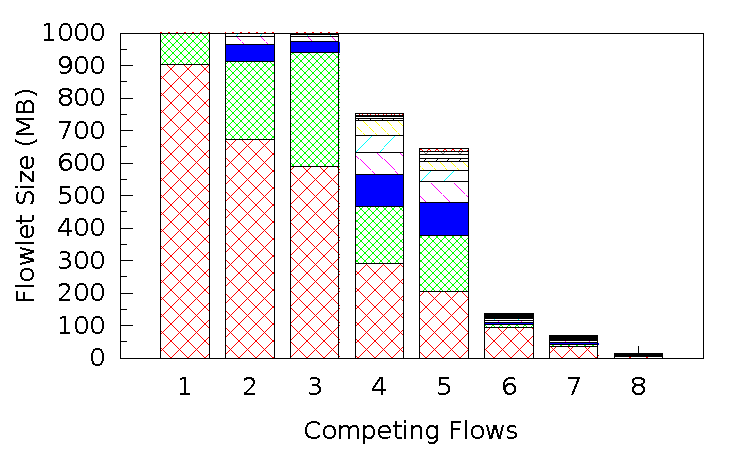
\includegraphics[width=0.7\textwidth]{presto/figures/flowlets/histo.pdf}
        \caption{Stacked histogram of flowlet sizes (in MB) for a 1 GB {\tt scp} file transfer. We vary the number of {\tt nuttcp}~\cite{nuttcp} background flows and
                denote them as {\em Competing Flows}. The size of each flowlet is shown within each bar, and flowlets
                are created whenever there is a 500 $\mu$s delay between segments. The top 10 flowlet sizes are shown here.
                We also analyzed the results of a 1 GB {\tt nuttcp}, {\tt ftp}, and a simple custom client/server transfer and found them
                to be similar. }
        \label{micro_flowlet_size}
\end{figure}

%\aditya{the following two paras don't flow well. they don't make a clear case for why flowlets is a bad idea and TSO segment level switching is a good idea. if reordering is the 100us flowlets' big problem then why not use our receiver-side reordering tricks with 100us flowlets? also it is not clear how were are overcoming reordering simply by relying on TSO segment switching}

%\eric{Rough estimates from our experiments with 100$\mu$s: ~90\% of flowlet sizes are 114KB or less with flowlets. ~00.1\% of flowlets are
%larger than 1 MB, with the largest ranging from 2.1-20.5MB. Some thoughts: (i) 100 $\mu$s flowlets can still have flowlet sizes larger 
%than switch buffers, which can cause congestion/loss when collision occur, (ii) given that flowlet with 100 $\mu$s does not prevent reordering,
%then why should we use flowlets at all? (iii) flowlets were really meant to have inactivity timers larger than the max difference in latency
%over any two paths, and buffer latency at one switch alone is ~4ms, so the use of flowlets on these small time scales is fundamentally
%flawed, (iv) flowlets are sensitive to traffic demand at sender, (v) flowlets are non-uniform in size, (vi) flowlets could break small 
%flows over multiple paths. Using TSO segment ensures: (i) small, uniform units of load-balancing, which means (ii) we are indenpendent
%of traffic demand, (iii) collisions are not a problem b/c TSO size is smaller than buffer size, (iv) most small flows are routed
%over the same path, (v) we do not impose too much computational overhead on sender/receiver and (vi) we still need to solve reordering.}

% Rough outline for next two paragraphs
% Problem with flowlets:
%  1. Sensitive to traffic patterns at the sender
%     a. In practice, we find this means the distribution of flowlet sizes is not uniform, and has a tail
%     b. These tails can still experience hash collisions, albeit less often.
%		i. congestion: lower throughput and to longer mice tail latencies
%  2. Needlessly break down small flows into several flowlets
%     a. Especially early in connection: 100us, 50 KB mice flows broken into 4-5 flowlets
%  3. Designed to be robust to reordering, but difficult to tune
%


Another possibility is to load balance on flowlets~\cite{conga,juniper-vcf}.  
A flow is comprised of a series of bursts, and a flowlet is created when
the inter-arrival time between two packets in a flow exceeds a threshold inactivity timer.  
In practice, inactivity timer values are between 100-500 $\mu$s~\cite{conga}. 
These values intend to strike a good balance between load balancing on a sub-flow level 
and acting as a buffer to limit reordering between flowlets.
Flowlets are derived from traffic patterns at the sender, and in practice this
means the distribution of flowlet sizes is not uniform. To analyze flowlet sizes, a simple experiment is shown in Figure~\ref{micro_flowlet_size}. 
We connect a sender and a receiver to a single switch and start an {\tt scp} transfer designed to 
emulate an elephant flow. Meanwhile, other senders are hooked up to the same switch and
send to the same receiver. We vary the number of these competing flows and show a stacked histogram of 
the top 10 flowlet sizes for a 1 GB {\tt scp} transfer with a 500 $\mu$s inactivity timer. 
The graph shows flowlet sizes can be quite large, with more than half the transfer being attributed
to a single flowlet for up to 3 competing flows. Using a smaller inactivity timer, such 100$\mu$s, helps (90\% of flowlet sizes are 114KB or less), but
does not prevent a long tail: 0.1\% of flowlets are larger than 1 MB, with the largest ranging from 2.1-20.5 MB.
Collisions on large flowlet sizes can lead to congestion.
The second problem with flowlets is that small inactivity thresholds, such as 100 $\mu$s, can lead to significant reordering.
Not only does this impact TCP performance (profiled in Section~\ref{sec:micro}), but it also needlessly 
breaks small flows into several flowlets. With only one flow in the network, we found a 50 KB
mice flow was broken into 4-5 flowlets on average. Small flows typically do not need to be
load balanced on a sub-flow level and need not be exposed to reordering.


%Another possibility is to load balance on flowlets~\cite{conga,juniper-vcf}.  A flow is typically comprised of a series of bursts, and each burst is defined as a flowlet. By monitoring the inter-arrival time of packets in a flow, one can easily define an inactivity timer to seperate flowlets.  In practice, intactivity timer values are between 100-500 $\mu$s~\cite{conga}. These values are intended to strike a good balance between creating enough opportunities to load balance on a sub-flow level and also ensure the reordering is limited at the destination due to the time buffer naturally incurred between flowlets.  We find, however, that it is difficult to strike a balance between achieving fine-grained, near-optimal load balancing and robustness against reordering. We perform a simple experiment in Figure~\ref{micro_flowlet_size}.  We connect a sender and a receiver to a single switch and start a transfer over an application designed to emulate an elephant flow ({\tt scp}). Meanwhile, we also hook up other senders to the same switch and have them send to the same reciever. We vary the number of competing flows and show a stacked histogram of the top 10 flowlet sizes for a 1 GB scp transfer with a 500 $\mu$s inactivity timer. \eric{Competing flows use nuttcp.} The graph shows flowlet sizes can be large, which means hash collisions can still occur on large flowlets.  Using a smaller timeout, such as 100 $\mu$s, creates smaller flowlets, but as we show in Section XXX, suffers from severe reordering that greatly reduces throughput and hurts applications.  \eric{mention creates congestion, which leads to lower thorughput and increase mice FCT latency}

% What do we want in sub-flow load balancing?
%  A. Want to move toward idealized ECMP: uniform sub-flow load balancing without the tail
%  B. Units should be as small as possible for fine-grained load balancing, but
%       not so small to be inefficient (TSO) or break small flows into parts
%  C. Independent of traffic patterns on sender
%  As a result, we settle on...

The shortcomings of the previous approaches lead us to reconsider on what granularity
load balancing should occur. 
%We take motivation from a best-case ECMP scenario. 
Ideally, sub-flow load balancing should be done on near uniform sizes.
%independent of traffic patterns on the sender to avoid long tails. 
Also, the unit of load balancing should be small to
allow for fine-grained load balancing, but not so small as to break small flows into 
many pieces or as to be a significant computational burden. As a result, we
propose load balancing on 64 KB units of data we call {\em flowcells}. Flowcells
have a number of advantages. First, the maximum segment size supported by TSO
is 64 KB, so flowcells provide a natural interface to high speed optimizations provided
by the NIC and OS and can scale to fast networking speeds. Second, an overwhelming fraction of mice flows are less than 64 KB in size
 and thus do not have to worry about reordering~\cite{benson10,vl2,kandula2009nature}.
Last, since most bytes in datacenter networks originate from elephant flows~\cite{kandula2009nature,benson10,dctcp},
this ensures that a significant portion of datacenter traffic is routed on uniform
sizes. While promising, this approach must combat reordering to be effective. 
Essentially we make a trade-off: 
%we provide line rate load balancing in the most effective
%manner as to avoid congestion and then handle reordering head-on at the receiver.
the sender avoids congestion by providing fine-grained, near-uniform load balancing,
and the receiver handles reordering to maintain line-rate.


%We highlight the challenges of this approach
%in the next subsection and provide a design to mitigate reordering problems in Section~\ref{sec:design}.

%In order to obtain fine-grained, near-optimal load balancing, we should stripe on a granularity
%that is indendpent of traffic patterns, near-uniform in size, and as small as possible while still
%scaling to fast network speeds.
%Therefore, we argue the TSO segment~\keqiang{what about saying maximum TSO segment size (64KB), each TSO segment's size is bounded by maximum TSO size} 
%is the natural granularity in which to load balance. Doing so
%provides several benefits. First, TSO segments are small and near-uniform in size, so an
%effective load-balancing scheme should be able to closely track the optimal case of per-packet
%load balancing, but without the additional computational overhead.
%Second, the TSO engine in the NIC will ensure that all packets created from a TSO segment will contain the same
%header information. We show in Section XXX how this is important to deal with reordering because
%we can easily impart metadata on all packets within a segment that help us distinguish loss from 
%ordering~\keqiang{all the packets within the same flowcell contain the same flowcell id.  
%"all packets created from a TSO segment will contain the same
%header information" is fine but a flowcell can contrain several TSO segments depending on TSO segment size}.
%Last, small flows less than 64 KB in size will actually be routed over the
%same path in the network, meaning a very large fraction of mice flows will not be routed on a subflow
%level and thus do not have to worry about reordering~\cite{benson10,vl2,kandula2009nature}~\keqiang{Around 90\% of datacenter flows' sizes are smaller than 64KB~\cite{benson10}, 
%meaning the overwhelming majority is load balanced like ECMP and we only need to engineering the left 10\%}.
%\eric{need to mention that we can combine segments as long as not above 64 KB, so not really
%per TSO segment. helps in small flows.}
%While promising, this approach has a major challenge: reordering. We highlight these challenges
%in the next subsection and provide a design to mitigate the problems in Section~\ref{sec:design}.

\tightparagraph{Per-Hop vs End-to-End Multipathing}
The last design consideration is whether multipathing should be done on a local, per-hop level (\eg{}ECMP), or
on a global, end-to-end level. In Presto, we choose the latter: pre-configured end-to-end paths
are allocated in the network and path selection (and thus multipathing) is realized by having the network edge
place flowcells onto these paths. 
Presto can be used to load-balance in an ECMP style per-hop manner, but the choice of end-to-end 
multipathing provides additional benefits due to greater control of how flowcells are mapped to
paths. Per-hop multipathing can be inefficient
under asymmetric topologies~\cite{wcmp}, and load-balancing on a global end-to-end level can allow
for weighted scheduling at the vSwitch to rebalance traffic. This is especially important when failure occurs.
The second benefit is flowcells can be assigned over multiple paths very evenly
by iterating over paths in a round-robin, rather than randomized, fashion. 

%As we show
%in Section~\ref{sec:micro}, randomization in per-hop multipathing can lead to "unluckiness" where
%multiple flowcells get sent to the same link over a small timescale by multiple flows. This transient congestion
%can lead to increased buffer occupancy and higher delays in the network. These benefits can
%fundamentally be provided at the per-hop level (\cite{wcmp} handles asymmetry), but require changes to networking firmware. 
%These considerations motivate us to utilize end-to-end multipathing, but Presto can also
%use per-hop multipathing when conveinent.

\subsection{Reordering Challenges}
%The above design decisions in Presto cause following main challenges:
Due to the impact of fine-grained, flowcell-based load balancing, Presto must account for reordering. Here, we 
highlight reordering challenges. The next section shows how Presto deals with these concerns.

%\tightparagraph{Soft Edge Distributed Load Balancing}
%There are two main challenges in implementing load balancing at the soft edge. First, the implementation
%must scale to fast networking speeds because networking at 10+ Gbps can have significant overhead if not carefully
%considered. Therefore, in order to achieve line rate, great care must be taken to ensure that load balancing
%schemes are light-weight, simple and can take advantage of optimizations provided by the NIC and OS.  
%The second major problem is how to load balance in a distributed fashion at the vSwitches in such
%a way that the load balancing performs well globally.
%Nodes must ensure they are spreading
%their traffic equally throughout the network, but in a low-overhead fashion that does not require detailed
%topographical information about the network, real-time traffic matrices, or strict coordination
%with other senders.

%\eric{several things to add: in presto, we can just make dumb edge decisions and not have to worry
%about (i) the traffic patterns, that is who else is sending, (ii) topology asymmetry. Basically,
%we want to highight that the vSwitch shouldn't require a lot of detailed network-wide information,
%but should be able to somehow still load balance in a way that performs very well globally.}

\tightparagraph{Reordering's Impact on TCP} The impact of reordering on TCP is well-studied~\cite{leung2007overview,paxson1997end}. 
Duplicate acknowledgments caused by reordering
can cause TCP to move to a more conservative sender state and reduce the sender's congestion window.
Relying on parameter tuning, such as adjusting the DUP-ACK threshold, is not ideal because 
increasing the DUP-ACK threshold increases the time to recover from real loss. Other TCP settings
such as Forward Acknowledgement (FACK) assume un-acked bytes in the SACK are lost and degrade
performance under reordering. 
A scheme that introduces reordering should not rely on careful configuration of TCP parameters
because (i) it is hard to find a single set of parameters that work effectively over multiple 
scenarios and (ii) datacenter tenants should not be forced to constantly tune their networking stacks.
Finally, many reordering-robust variants of TCP have been proposed~\cite{rr-tcp,blanton2002making,tcp-pr}, but
as we will show, GRO becomes ineffective under reordering. Therefore, reordering should
be handled below the transport layer.

\tightparagraph{Computational Bottleneck of Reordering}
Akin to TSO, Generic Receive Offload (GRO) mitigates the computational burden of receiving
1500 byte packets at 10 Gbps. GRO is implemented in the kernel of the hypervisor,
and its handler is called directly by the NIC driver. It is responsible
for aggregating packets into larger segments that are pushed up to OVS and the TCP/IP stack. 
GRO is implemented in the Linux kernel and is used even without virtualization. Similar
functionality can be found in Windows (RSC~\cite{ms-rsc}) and hardware (LRO~\cite{grossman2005large}).

Because modern CPUs use aggressive prefetching, the cost of receiving
TCP data is now dominated by per-packet, rather than per-byte, operations.
As shown by Menon~\cite{optimize-tcp-receive},  the majority of this overhead comes from
buffer management and other routines not related to protocol processing, and therefore 
significant computational overhead can be avoided by aggregating "raw" packets from
the NIC into a single {\tt sk\_buff}.
%\footnote{Refer to~\cite{linuxgro,optimize-tcp-receive} for detailed study and explanation}
Essentially, spending a few cycles to aggregate packets within GRO creates less segments for
TCP and prevents having to use substantially more cycles at higher layers in the networking stack.
Refer to~\cite{linuxgro,optimize-tcp-receive} for detailed study and explanation.

To better understand the problems reordering causes, a brief description of  
the TCP receive chain in Linux follows. First, interrupt coalescing allows the NIC to create an interrupt for a batch of packets~\cite{mogul1997eliminating,understanding-linux-network},
which prompts the driver to poll the packets into an aggregation queue. Next, the driver
invokes the GRO handler, located in the kernel, which
{\em merges} the packets into larger segments. The merging continues,
possibly across many polling events, until a segment
reaches a threshold size, a certain age, or cannot be combined with the incoming packet. Then, the
combined, larger segment is {\em pushed up} to the rest of the TCP/IP networking stack. The GRO process is
done on a per-flow level. With GRO disabled, throughput drops to around
5.7-7.1 Gbps and CPU utilization spikes to 100\% (Section~\ref{sec:micro} and~\cite{bullettrains}). 
Receive offload algorithms, whether in hardware (LRO)~\cite{grossman2005large,open-lro} or in software (GRO), are usually
{\em stateless} to make them fast: no state is kept beyond the segment being merged.


%\begin{figure}[!htb]
%        \centering
%  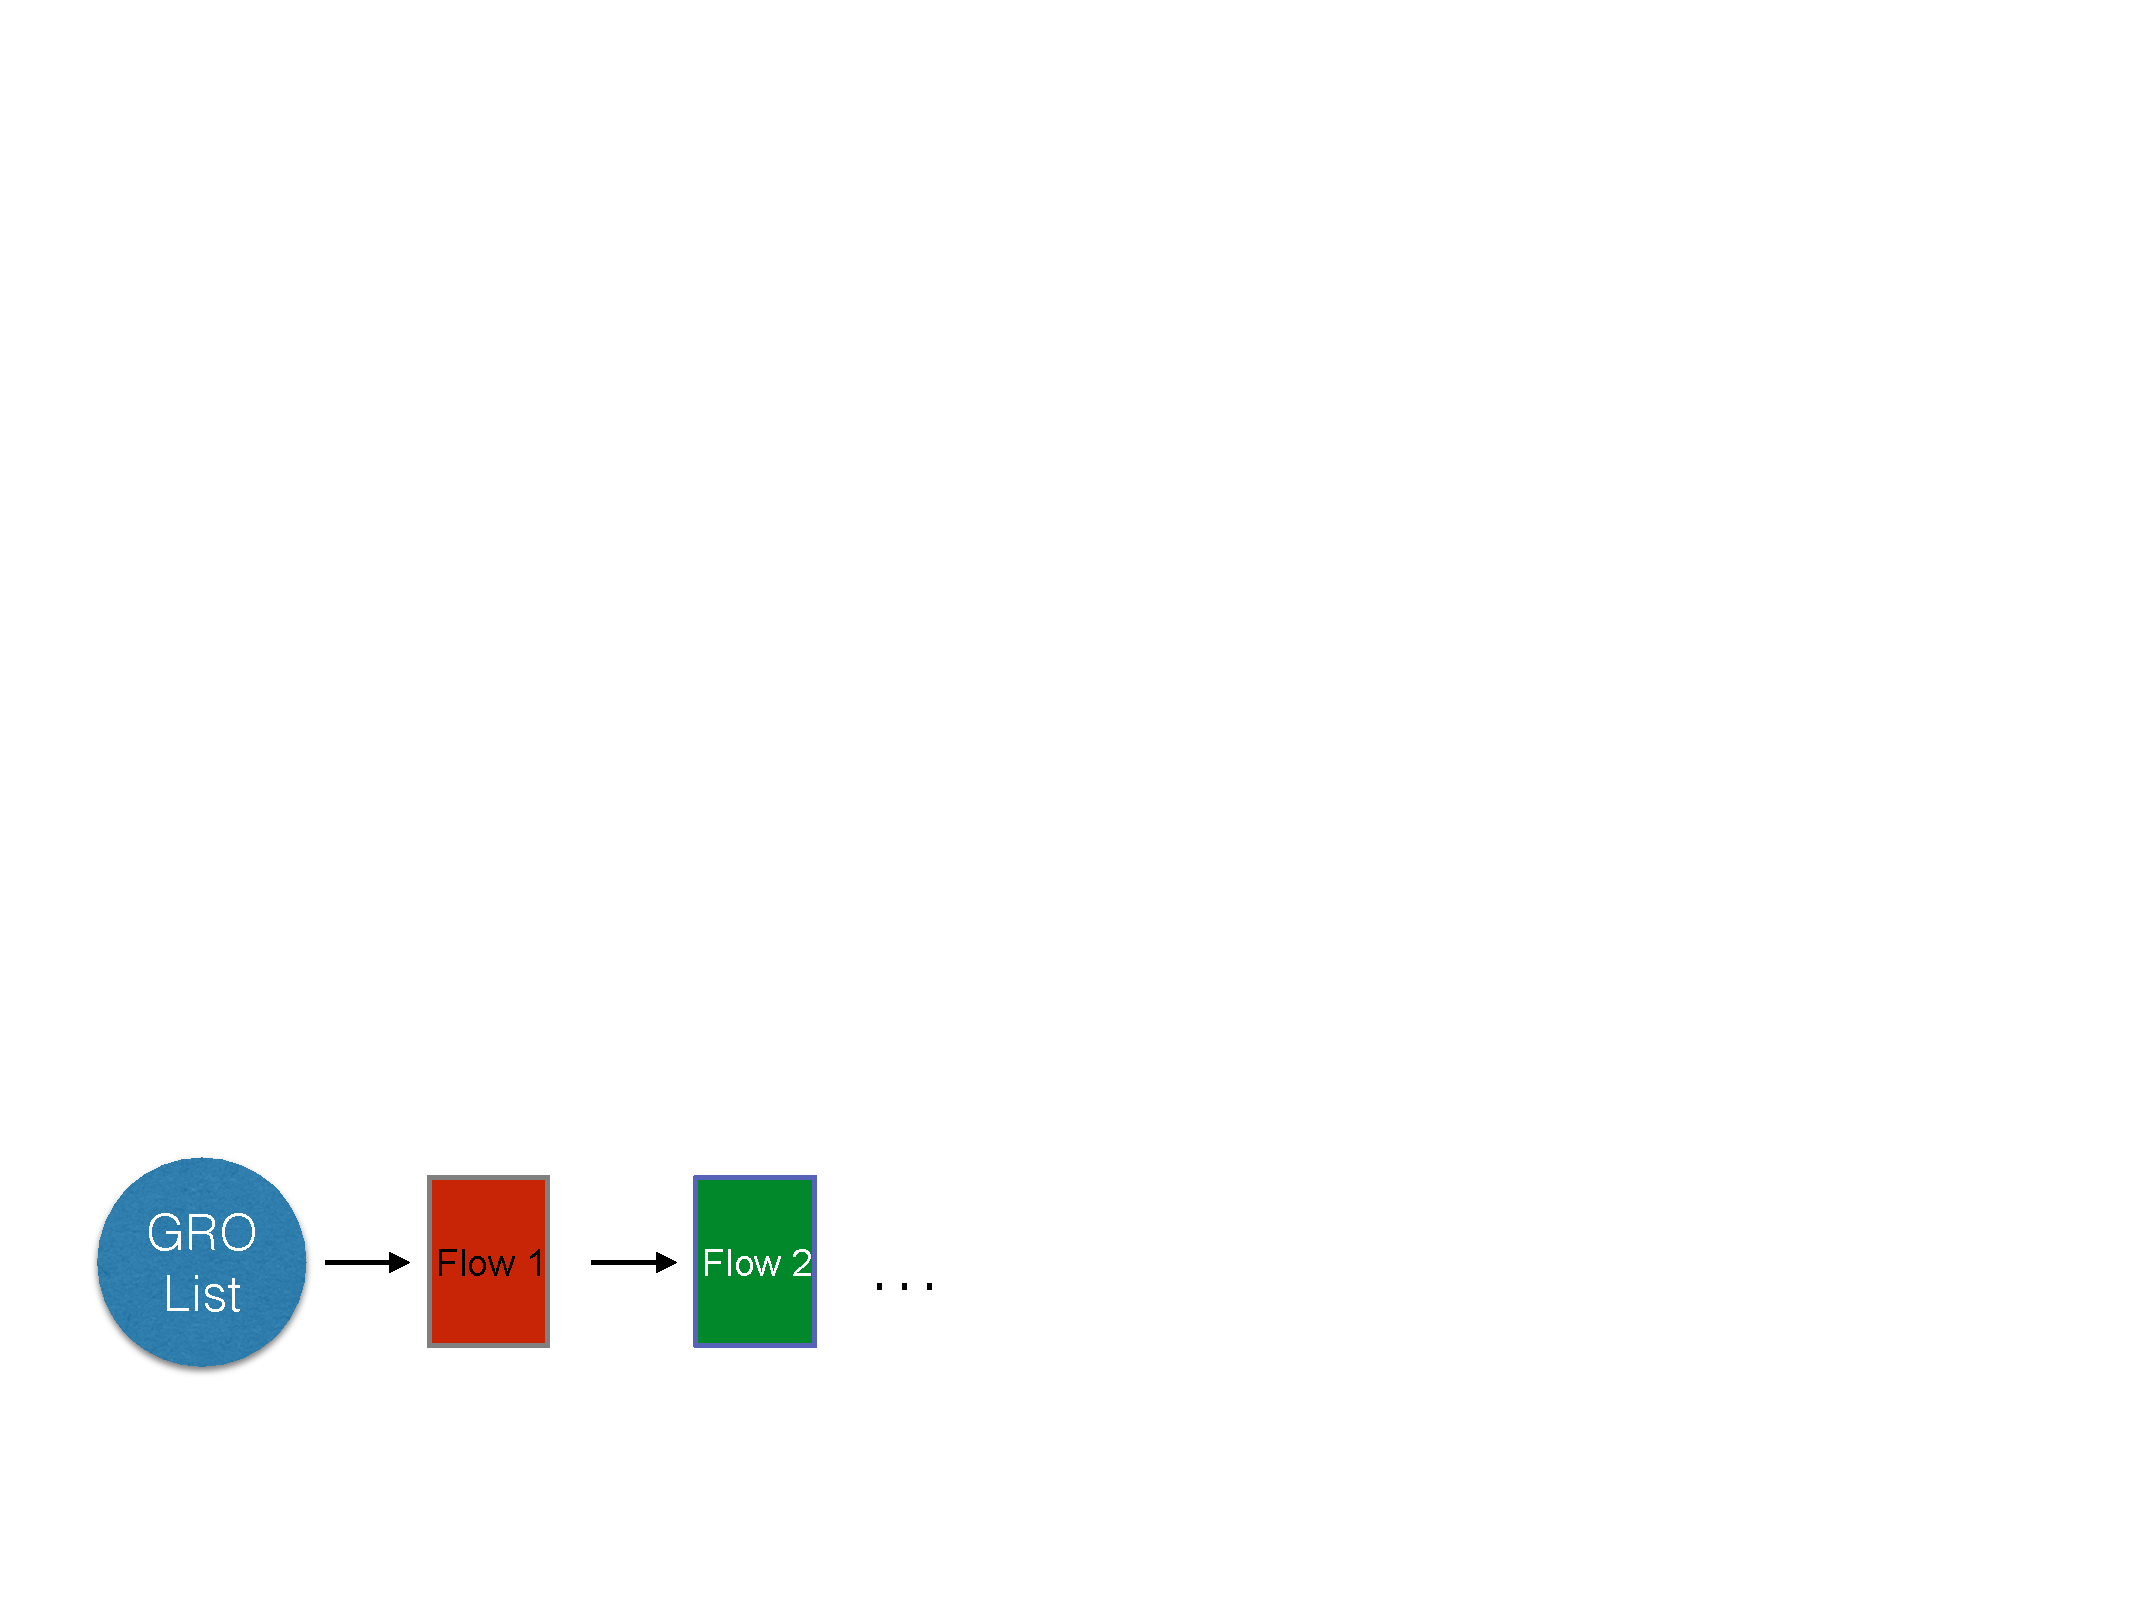
\includegraphics[width=0.45\textwidth]{presto/figures/gro-design/gro.pdf}
%        \caption{GRO design. FIX ME!}
%        \label{gro-design}
%\end{figure}

\begin{figure}[!t]
        \centering
  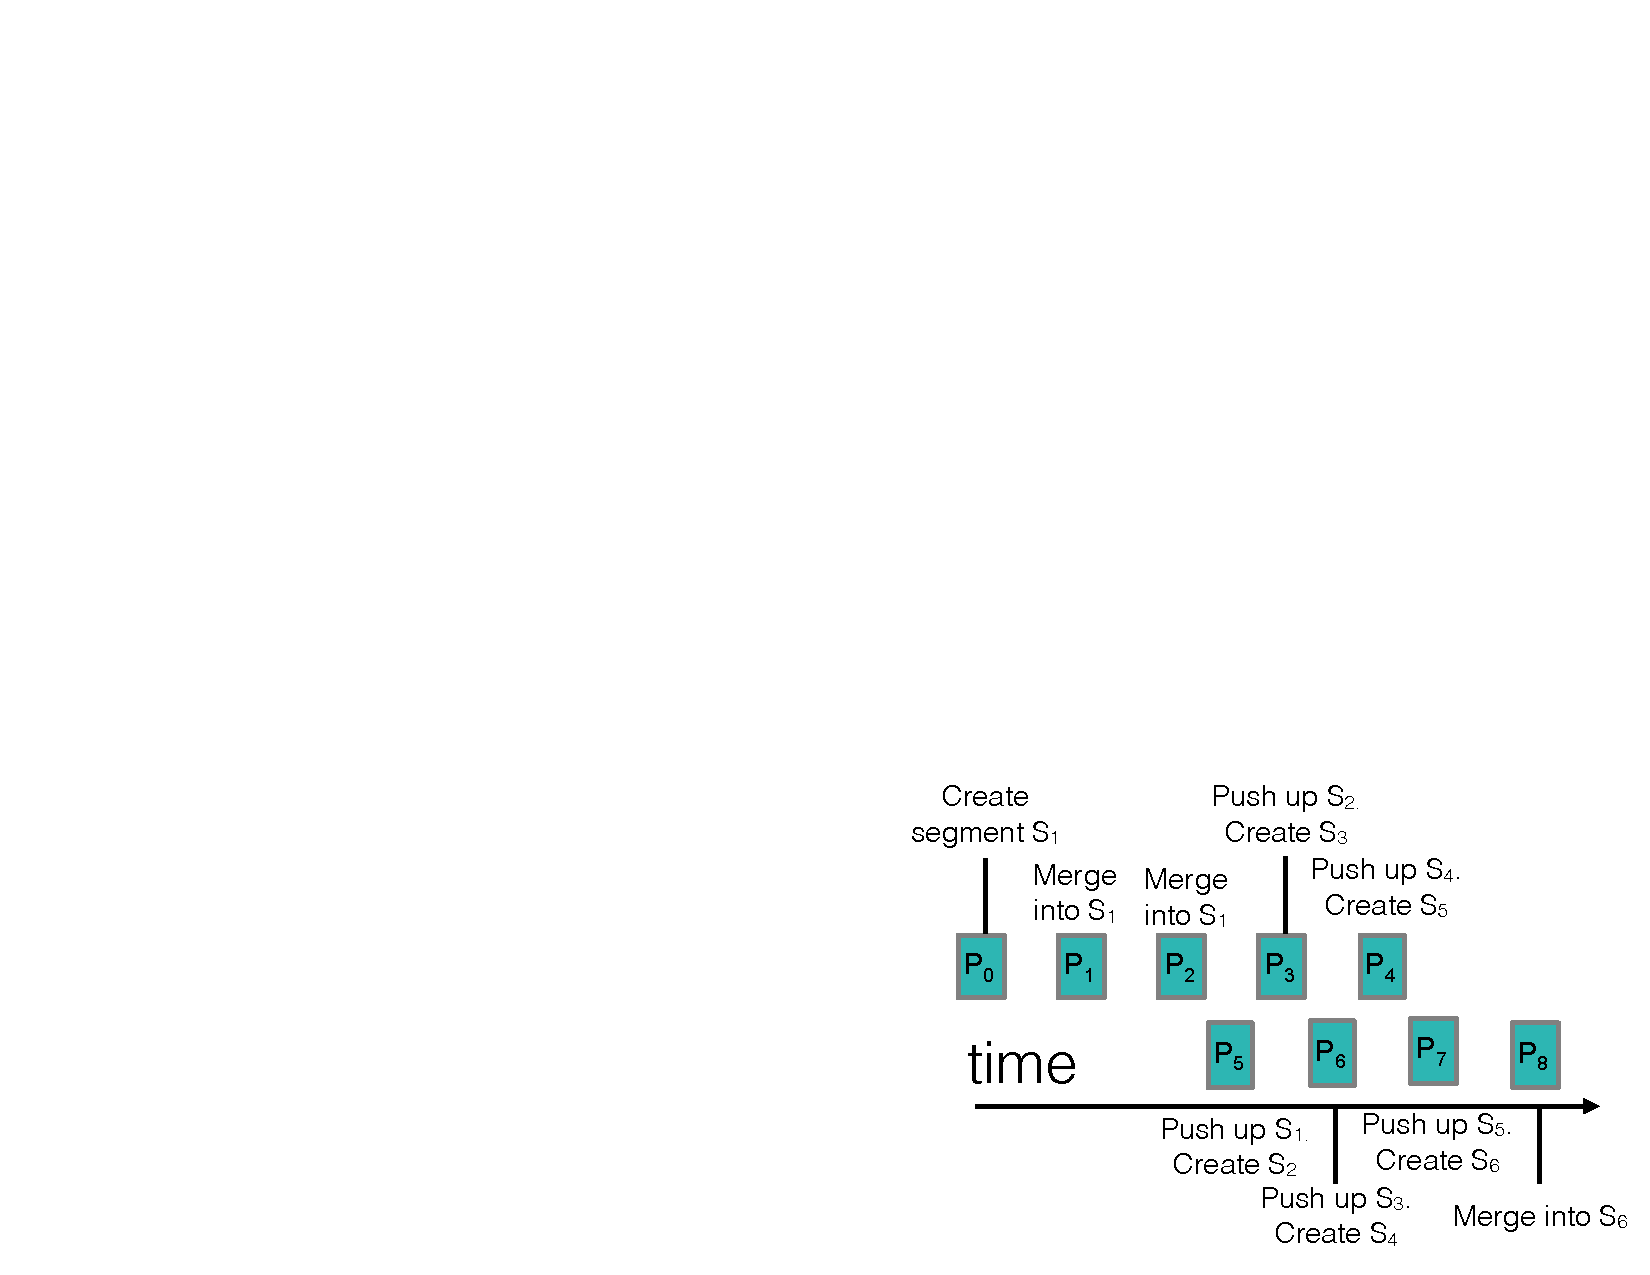
\includegraphics[width=0.7\textwidth]{presto/figures/gro-design/gro-break.pdf}
        \caption{GRO pushes up small segments ($S_i$) during reordering.}
        \label{gro-break}
\end{figure}


We now uncover how GRO breaks down in the face of reordering. Figure~\ref{gro-break} shows the impact of reordering on GRO.  Reordering does not allow the segment to grow: each reordered packet cannot be merged with the existing segment, and thus the previously created segment must be pushed up. With extreme reordering, GRO is effectively disabled because small MTU-sized segments are constantly pushed up. This causes (i) severe computational overhead and (ii) TCP to be exposed to significant amounts of reordering. We term this the {\em small segment flooding} problem.

Determining where to combat the reordering problem has not previously taken the small segment flooding problem into account.  Using a reordering buffer to deal with reordered packets is a common solution (\eg{}works like~\cite{drb} re-sort out-of-order packets in a shim layer below TCP), but a buffer implemented above GRO cannot prevent small segment flooding.  Implementing a buffer below GRO means that the NIC must be changed, which is (i) expensive and cumbersome to update and (ii) unlikely to help combat reordering over multiple interrupts.

In our system, the buffer is implemented in the GRO layer itself.  We argue this is a natural location because GRO can
directly control segment sizes while simultaneously limiting the impact of reordering. 
Furthermore, GRO can still be applied on packets pushed up from LRO, which means hardware doesn't have to be modified
or made complex.
Implementing a better GRO algorithm has multiple challenges. The algorithm should be light-weight to scale to fast networking speeds. Furthermore, an ideal scheme should be able to distinguish loss from reordering.  When a gap in sequence numbers is detected (\eg{}when $P_5$ is received after $P_2$ in Figure~\ref{gro-break}), it is not obvious if this gap is caused from loss or reordering.  If the gap is due to reordering, GRO should not push segments up in order to try to wait to receive the missing gap and merge the missing packets into a preestablished segment.  If the gap is due to loss, however, then GRO should immediately push up the segments to allow TCP to react to the loss as fast as possible. Ideally, an updated GRO algorithm should ensure TCP does not perform any worse than a scheme with no reordering. Finally, the scheme should adapt to prevailing network conditions, traffic patterns and application demands.




\chapter{Edge-based Load Balancing for Fast Datacenter Networks}

\section{Introduction}
\label{section:intro}

Datacenter networks must support an increasingly diverse set of
workloads.
Small latency-sensitive flows to support real-time applications such
as search, RPCs, or gaming share the network with large
throughput-sensitive flows for video, big data analytics, or VM
migration.
Load balancing the network is crucial to ensure operational efficiency
and suitable application performance.
Unfortunately, popular flow-hashing-based load balancing schemes,
\eg{}, ECMP, cause congestion when hash collisions
occur~\cite{hedera,dc-mptcp,planck,vmware,detail,packetspray,drb} and
perform poorly in asymmetric topologies~\cite{conga,wcmp}.

A variety of load balancing schemes aim to address the
problems of ECMP.
Centralized schemes, such as Hedera~\cite{hedera} and
Planck~\cite{planck}, collect network state and reroute elephant flows
when collisions occur.
These approaches are fundamentally reactive to congestion, and are
very coarse-grained due to the large time constants of their control
loops~\cite{hedera} or require extra network
infrastructure~\cite{planck}.
Transport layer solutions such MPTCP~\cite{mptcp}, can
react faster but require widespread adoption and are difficult to
enforce in multi-tenant datacenters where customers often deploy
customized virtual machines (VMs).
%Also, our experiments in Section~\ref{sec:micro}, ~\ref{sec:eval} and 
%CONGA~\cite{conga} show MPTCP has brittle performance in many workloads. 
In-network reactive distributed load balancing schemes, e.g.,
CONGA~\cite{conga} and Juniper VCF~\cite{juniper-vcf}, can be
effective but require specialized networking hardware.
%~\cite{conga,juniper-vcf,detail,packetspray}.
%NOTE: where does Mahout go? DCTCP?

%The design of above schemes ignore recent trends in datacenter network design. Complex newtork
%hardware leads to extra cost, vendor lock-in, and increased down-time. 

The shortcomings of the above approaches cause us to re-examine the design space for load balancing in datacenter networks. ECMP, despite its limitations, is a highly practical solution due to its proactive nature and stateless behavior.
%It provides clear benefits in robustness and simplicity 
%compared to the complex and often fragile reactive schemes. 
Conceptually, ECMP's flaws are not internal to its operation but are caused by asymmetry in network topology (or capacities) and variation in flow sizes. {\em In a symmetric network topology
where all flows are ``mice'', ECMP should provide near optimal load balancing}; indeed, prior work~\cite{conga,flowlet} has shown the traffic imbalance ECMP imposes across links goes down with an increase in the number of flows and a reduction in the variance of the flow size distribution. 

Can we leverage this insight to design a good proactive load balancing scheme without requiring special purpose hardware or modifications to end-point transport? The system we propose answers this in the affirmative. It relies on the datacenter network's {\em software edge} to transform arbitrary sized flows into a large number of near uniformly sized small sub-flows, and to proactively spread those uniform data units over the network in a balanced fashion. Our scheme is fast (works at 10+ Gbps), and doesn't require network stack configurations that may not be widely supported outside the datacenter (such as increasing MTU sizes). We piggyback on recent trends where several network functions, \eg{}, firewalls and application-level load balancers, are moving into hypervisors and software virtual switches on end-hosts~\cite{nv-mtd,ovs-extending}. Our paper makes a strong case for moving network load balancing functionality out of the datacenter network hardware and into the software-based edge.

% we really need expensive (and often fragile) congestion-aware reactive techniques like~\cite{hedera,mptcp,conga} to achieve load balancing in datacenter networks, or can we achieve a similar level of functionality by
% %1) adding symmetry to network 
% We argue that it is practical, cheaper, robust, and more efficient to do the latter. 

%It is important that such schemes not require any changes to the transport
%layer, extra network infrastructure or expensive network switches. 
\iffalse
Fortunately, many commonly deployed network topologies like 2-tier folded Clos (leaf-spine) already meet the network symmetry 
requirements though asymmetry may occur due to failures and should be handled. The main challenge then is to achieve uniformity 
in flow sizes i.e. a mechanism that can efficiently multiplex and de-multiplex logical flows into a more uniformly sized smaller 
sub-flow units. This mapping and the load balancing of the resulting units should ideally be done 
in the network itself instead of transport layer.
\fi
%We design our system to load balance arbitrary sized flows as near uniformly sized sub-flow units. 

%\aditya{this para can go - In the design of such a system, we draw 
%inspiration from network virtualization~\cite{nv-mtd,ovs-extending} and similar recent trends where several network functions (e.g. distributed firewall) 
%are being moved to the soft edge. We claim that hypervisors and soft virtual switches at the network edges are the ideal places to 
%implement the load balancing logic. Schemes like CONGA~\cite{conga} and Juniper VCF~\cite{juniper-vcf} aim to load balance in the "fabric", but
%ignore the fact that in many commercial datacenters, the {\em soft-edge} (\eg{} Open vSwitch~\cite{ovs-website}) is increasingly part of the 
%fabric as well~\cite{nv-mtd}.}

%See Nicira's NSDI 2014 paper~\cite{nv-mtd}. Conga's notion of fabric extends just to the leaf switches.


% The main thesis of this paper is to answer whether {\em fine-grained, non-reactive, near-optimal load balancing is implementable
% at the soft-edge}~\keqiang{better to say pro-active?}. Our design goals are that the system should not require changes to networking hardware or 
% additional networking infrastructure. Furthermore, the design should not require changes to the transport layer or complex transport 
% layer tuning. Finally, 

%
%the Fabric paper~\cite{casado2012fabric}, which advocates for a combined intelligent
%(software?~\keqiang{Yes, Fabric paper wrote "at present much edge forwarding in datacenters is done in software 
%by the host's general-purpose CPU", last page, second paragraph (top left)}) network edge with a simple label-switched core. 
%
%

Several challenges arise when employing the edge to load balance the network
on a sub-flow level. Software is slower than hardware, so operating at 10+ Gbps speeds means
algorithms must be simple, light-weight, and take advantage of optimizations in
the networking stack and offload features in the NIC. Any sub-flow level load balancing should also be 
robust against reordering.
%Due to variations in the end host networking stack~\cite{bullettrains},
%obtaining the "ground truth" of packet timing characteristics on the wire is difficult~\keqiang{vSwitch is below TCP/IP, 
%so what vSwitch observes is close to "groud truth". Undertand that you want to make a soft argument on flowlet here}. 
%We show flowlet-based
%load balancing schemes can be difficult to implement and tune in software, and therefore we must find an alternative
%approach to load balance the network while being robust against reordering. 
As shown in Section~\ref{sec:background}, 
reordering not only impacts TCP's congestion control mechanism, but also imposes significant computational
strain on hosts, effectively limiting TCP's achievable bandwidth if not properly controlled. Last, the approach must be 
resilient to hardware or link failures and be adaptive to network asymmetry.

%On the other hand, an open, software-based approach
%prevents extra hardware cost and vendor lock-in, and allows for simplified network management. These issues
%are cited as major concerns today (cite FB interview).
%Thanks to projects like Open vSwitch, soft-switching platforms are fast, mature, open source, adapted widely, remotely
%configurable, SDN-enabled, and feature-rich~\cite{nv-mtd}. Last, an intelligent soft-edge architechture
%is designed to be flexible and easily evolvable~\cite{casado2012fabric}.

% XXX - maybe we can argue something about cost: we need less over-subscription because we don't have to worry about burst/collisions/congestion as much.
% FB, for example, has 10 to 40 Gbps links (google altoona).
%Flexible: simplified core with software edge is evolvable. Consistent-updates~\cite{shadow-mac}.
%Soft-switching in end-hosts is already very mature and feature-rich,
%and some very sophisticated actions can be taken there. We're piggy-backing on this trend.
%
%{ \em If we arrive at a point where the edge processing is done in software
%and the core in simple hardware, then the entire infrastructure
%becomes much more evolvable} ---Martin Casado et al.~\cite{casado2012fabric}
%
%~\keqiang{found a good argument made in Shadow MAC paper, copied below}
%A recent position paper by Casado et al.~\cite{casado2012fabric} suggests that 
%next-generation networks should combine an intelligent network edge with a label-switched core. 
%Casado et al. arrive at this conclusion based on separating the concerns of end points, switches, and operators. 
%We arrive at the same conclusion based a different line of reasoning, which lends credence to the notion that 
%SDN-enabled networks should be architected in this fashion.
%
%Challenges: End-host overheard/impact on apps; keeping up with 10G speeds; solving packet reordering without touching transport layer;
%resilient to hardware or link failures, adaptive to network asymmetry.

To this end, we build a proactive load balancing system called Presto.
Presto utilizes vSwitches to break flows into discrete units of packets, called 
{\em flowcells}, and distributes them evenly 
to near-optimally load balance the network. 
Presto uses the maximum TCP Segment Offload (TSO) size (64 KB) as flowcell granularity, 
allowing for fine-grained load balancing at network speeds of 10+ Gbps.  
%Flowcells
%are near uniform in size because they are mostly independent of traffic patterns at the sender and 
%provide a natural interface to offload optimizations provided in the NIC and OS, allowing
%for fine-grained load balancing to scale to network speeds of 10+ Gbps. 
%Pushing the limits of fine-grained load balancing in fast networks means that reordering 
%must be addressed, 
%and therefore 
To combat reordering, we modify the Generic Receive Offload (GRO) handler
in the hypervisor OS to mitigate the computational burden imposed by reordering
and prevent reordered packets from being pushed up the networking stack.
Finally, we show Presto can load balance the network
in the face of asymmetry and failures.


%with input from a centralized controller, vSwitches in Presto can load balance the network
%in the face of asymmetry, without requiring detailed global information about the 
%network topology or traffic patterns at each vSwitch.
%Presto can improve throughput, latency and fairness in the network and reduce mice flow completion
%time tail latencies.

Our paper makes the following contributions:
\begin{enumerate}

\item We design and implement a system, called Presto, that near-optimally load balances
links in the network. We show that such a system can be built with no changes to the transport
layer or network hardware, and scales to 10+ Gbps networking speeds.
%Presto  
%improves throughput, latency and fairness in the network and reduces flow completion time tail latencies
%for mice flows.
%\item We show that such a system can be built with no changes to the transport
%layer or within network hardware. Unlike previous approaches with similar design goals~\cite{drb}, we 
%ensure our approach scales to network speeds higher than 1 Gbps.
Our approach makes judicious use of middleware
already implemented in most hypervisors today: Open vSwitch and the TCP receive offload engine in the OS
(Generic Receive Offload, GRO, in the Linux kernel).\footnote{Also known as Receive Segment Coalescing (RSC)~\cite{ms-rsc}, or in hardware, Large Receive Offload (LRO)~\cite{grossman2005large}} 

%We show our approach can work in both SDN and non-SDN environments.
\item We uncover the importance of GRO on performance when packets are reordered.
At network speeds of 10+ Gbps, current GRO algorithms are unable to sustain line rate under 
severe reordering due to extreme computational overhead, and hence 
per-packet load-balancing approaches~\cite{drb,packetspray} need to be reconsidered. We
improve GRO to prevent reordering while ensuring computational overhead is limited.
%Our scheme can distinguish loss from reordering and adapt to prevailing network conditions.
%These techniques are criticial to ensure we minimize the time waiting for lost packets, while
%being robust against exposing reordering to higher network layers.  
We argue
GRO is the most natural place to handle reordering because it can mask
reordering in a light-weight manner while simultaneously limiting CPU overhead by having a direct impact
on the segment sizes pushed up the networking stack.
%Need to sell this more: this is the only place we should really do it because it has
%direct impact on packet sizes, and thus CPU overhead. We also need to talk about mechanisms
%we create to distinguish loss from reordering.

\item Presto achieves near-optimal load balancing in a proactive manner. For that, it leverages symmetry in 
the network topology to ensure that all paths between a pair of hosts are equally congested. 
However, asymmetries can arise due to failures. We demonstrate Presto can recover from network failures and adapt to asymmetric 
network topologies using a combination of fast failover and weighted multipathing at the network edge.


\item Finally, we evaluate Presto on a real 10 Gbps testbed. Our experiments show Presto
outperforms existing load balancing schemes (including flowlet switching, ECMP, MPTCP) and 
is able to track the performance of a single, non-blocking switch (an optimal case) within a few percentage points
over a variety of workloads, including trace-driven. Presto improves throughput, latency and fairness in the network and 
also reduces the flow completion time tail for mice flows.

\end{enumerate}



\section{Design Decisions and Challenges}
\label{sec:background}

In Presto, we make several design choices to 
build a highly robust and scalable system that provides near optimal load 
balancing without requiring changes to the transport layer or switch hardware. We 
now discuss our design decisions.


\subsection{Design Decisions}

\tightparagraph{Load Balancing in the Soft Edge} A key design decision in Presto 
is to implement the functionality in the soft edge (\ie, the vSwitch and hypervisor) of 
the network. 
%should we motivate why not to do it in hardware?
%A current trend in datacenter design is to utilize network equipment from 
%original design manufacturers (ODMs) in order to simplify and customize
%the network. This has been reported to significantly reduce costs and improve
%network performance~\cite{aws-peek}.
%Motivation here is that network is becoming very simple, and functionalities
%are being moved to an intelligent edge. Examples are VMWare/NSDI, Fabric, NFV in vSwitch,
%SDNs/OpenFlow, 
% Given recent advancements in this space\eric{what advancements? can we be more specific
% in order to provide better motivation?}, we believe the soft edge is the best 
% place to deploy new network functions, such as load balancing, in a scalable and 
% distributed manner.\eric{is this a new position? vmware nsdi paper...}
The vSwitch occupies a unique position in the networking stack 
in that it can easily modify packets without requiring any changes to customer VMs or transport layers.
Functionality built into the vSwitch can be made aware of the underlying hardware offload
features presented by the NIC and OS, meaning it can be fast.
Furthermore, an open, software-based approach prevents extra hardware cost and vendor 
lock-in, and allows for simplified network management. 
These criteria are important for providers today~\cite{aws-peek}.
Thanks to projects like Open vSwitch, 
soft-switching platforms are now fast, mature, open source, adopted widely, remotely 
configurable, SDN-enabled, and feature-rich~\cite{ovs-edge,nv-mtd,pfaff2015design}. Presto is built on these 
platforms.

\tightparagraph{Reactive vs Proactive Load Balancing} The second major design decision in 
Presto is to use a proactive approach to congestion management. Bursty 
behavior can create transient congestion that must be reacted to 
before switch buffers overflow to prevent loss (timescales range from 100s of $\mu$s 
to \textasciitilde{}4 ms~\cite{planck}). This requirement renders most of the centralized reactive schemes ineffective
as they are often too slow to react to any but the largest network events,~\eg{}, link failures. 
%Not reacting to transient congestion can increase tail latencies.
Furthermore, centralized schemes can hurt performance when rerouting
flows using stale information.
%By reacting on a different scale than the congestion, centralized schemes may reroute flows
%on stale information, which can hurt performance.
Distributed reactive schemes like MPTCP~\cite{mptcp} and 
CONGA~\cite{conga} can respond to congestion at faster timescales, but have a high barrier to deployment.
Furthermore, distributed reactive schemes must take great care to avoid oscillations.
Presto takes a proactive, correct-by-design approach to congestion management. 
That is, if small, near-uniform portions of traffic are equally
balanced over a symmetric network topology, then the load-balancing can remain agnostic to congestion and
leave congestion control to the higher layers of the networking stack.
%then we don't need to 
%be reactive to congestion.
Presto is only reactive to network events such as link failures. Fortunately, 
the larger timescales of reactive feedback loops are sufficient in these scenarios. 

\tightparagraph{Load Balancing Granularity} ECMP has been shown to be ineffective at load balancing the network, and thus many schemes advocate load balancing at a finer granularity than a flow~\cite{drb,conga,juniper-vcf,packetspray}. A key factor impacting the choice of granularity is operating at high speed. 
%and ensuring suitable application level performance.
%Implementing fine-grained, near-uniform load balancing in 10+ Gbps networks
%is difficult.
Operating at 10+ Gbps incurs great computational overhead, and therefore host-based load balancing schemes
must be fast, light-weight and take advantage of optimizations provided in the networking stack.
For example, per-packet load balancing techniques~\cite{drb} cannot be
employed at the network edge because TSO does not work on a per-packet
basis. TSO, commonly supported in OSes and NICs, allows for large TCP segments (typically 64 KB in size)
to be passed down the networking stack to the NIC. The NIC breaks the segments into MTU-sized packets and copies and computes
header data, such as sequence numbers and checksums. When TSO is disabled, a host incurs 100\% utilization of one CPU core and can only achieve
around 5.5 Gbps~\cite{bullettrains}. Therefore, per-packet schemes are unlikely to scale to fast networks without hardware support.
Limiting overhead by increasing the MTU is difficult because
VMs, switches, and routers must all be configured appropriately, and traffic
leaving the datacenter must use normal 1500 byte packets. Furthermore, per-packet schemes~\cite{drb,packetspray} are likely to
introduce significant reordering into the network.
%Achieving line rate at 10 Gbps is nontrivial because dealing
%with so many 1500 byte MTU-sized packets at varying layers
%of the networking stack causes significant computational overhead.
%Therefore, modern operating systems and network adapters have many
%optimizations to help burden the load.
%On the sender side, TCP Segmentation Offload (TSO)~\footnote{Generically known as large segment offload or generic segmentation offload}
%is designed to allow the TCP/IP stack to deal with large TCP segments. Segments, up to 64 KB in size, are passed
%from the application layer all the way down to the NIC, which in turn breaks the large segment down into 1500 byte packets.
%The NIC copies and calculates the header information, such as checksums and sequence numbers.
%This allows the computational burden to be substainally lessened, and therefore rates of 10+
%Gbps can be achieved. With TSO disabled, achievable 10 Gbps throughput drops to around 5.5 Gbps~\cite{bullettrains}.



\begin{figure}[t]
        \centering
  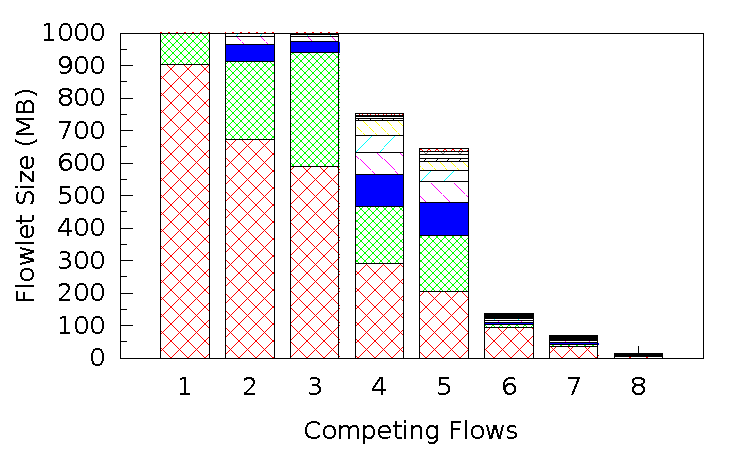
\includegraphics[width=0.45\textwidth]{presto/figures/flowlets/histo.pdf}
        \caption{Stacked histogram of flowlet sizes (in MB) for a 1 GB {\tt scp} file transfer. We vary the number of {\tt nuttcp}~\cite{nuttcp} background flows and
                denote them as {\em Competing Flows}. The size of each flowlet is shown within each bar, and flowlets
                are created whenever there is a 500 $\mu$s delay between segments. The top 10 flowlet sizes are shown here.
                We also analyzed the results of a 1 GB {\tt nuttcp}, {\tt ftp}, and a simple custom client/server transfer and found them
                to be similar. }
        \label{micro_flowlet_size}
\end{figure}

%\aditya{the following two paras don't flow well. they don't make a clear case for why flowlets is a bad idea and TSO segment level switching is a good idea. if reordering is the 100us flowlets' big problem then why not use our receiver-side reordering tricks with 100us flowlets? also it is not clear how were are overcoming reordering simply by relying on TSO segment switching}

%\eric{Rough estimates from our experiments with 100$\mu$s: ~90\% of flowlet sizes are 114KB or less with flowlets. ~00.1\% of flowlets are
%larger than 1 MB, with the largest ranging from 2.1-20.5MB. Some thoughts: (i) 100 $\mu$s flowlets can still have flowlet sizes larger 
%than switch buffers, which can cause congestion/loss when collision occur, (ii) given that flowlet with 100 $\mu$s does not prevent reordering,
%then why should we use flowlets at all? (iii) flowlets were really meant to have inactivity timers larger than the max difference in latency
%over any two paths, and buffer latency at one switch alone is ~4ms, so the use of flowlets on these small time scales is fundamentally
%flawed, (iv) flowlets are sensitive to traffic demand at sender, (v) flowlets are non-uniform in size, (vi) flowlets could break small 
%flows over multiple paths. Using TSO segment ensures: (i) small, uniform units of load-balancing, which means (ii) we are indenpendent
%of traffic demand, (iii) collisions are not a problem b/c TSO size is smaller than buffer size, (iv) most small flows are routed
%over the same path, (v) we do not impose too much computational overhead on sender/receiver and (vi) we still need to solve reordering.}

% Rough outline for next two paragraphs
% Problem with flowlets:
%  1. Sensitive to traffic patterns at the sender
%     a. In practice, we find this means the distribution of flowlet sizes is not uniform, and has a tail
%     b. These tails can still experience hash collisions, albeit less often.
%		i. congestion: lower throughput and to longer mice tail latencies
%  2. Needlessly break down small flows into several flowlets
%     a. Especially early in connection: 100us, 50 KB mice flows broken into 4-5 flowlets
%  3. Designed to be robust to reordering, but difficult to tune
%


Another possibility is to load balance on flowlets~\cite{conga,juniper-vcf}.  
A flow is comprised of a series of bursts, and a flowlet is created when
the inter-arrival time between two packets in a flow exceeds a threshold inactivity timer.  
In practice, inactivity timer values are between 100-500 $\mu$s~\cite{conga}. 
These values intend to strike a good balance between load balancing on a sub-flow level 
and acting as a buffer to limit reordering between flowlets.
Flowlets are derived from traffic patterns at the sender, and in practice this
means the distribution of flowlet sizes is not uniform. To analyze flowlet sizes, a simple experiment is shown in Figure~\ref{micro_flowlet_size}. 
We connect a sender and a receiver to a single switch and start an {\tt scp} transfer designed to 
emulate an elephant flow. Meanwhile, other senders are hooked up to the same switch and
send to the same receiver. We vary the number of these competing flows and show a stacked histogram of 
the top 10 flowlet sizes for a 1 GB {\tt scp} transfer with a 500 $\mu$s inactivity timer. 
The graph shows flowlet sizes can be quite large, with more than half the transfer being attributed
to a single flowlet for up to 3 competing flows. Using a smaller inactivity timer, such 100$\mu$s, helps (90\% of flowlet sizes are 114KB or less), but
does not prevent a long tail: 0.1\% of flowlets are larger than 1 MB, with the largest ranging from 2.1-20.5 MB.
Collisions on large flowlet sizes can lead to congestion.
The second problem with flowlets is that small inactivity thresholds, such as 100 $\mu$s, can lead to significant reordering.
Not only does this impact TCP performance (profiled in Section~\ref{sec:micro}), but it also needlessly 
breaks small flows into several flowlets. With only one flow in the network, we found a 50 KB
mice flow was broken into 4-5 flowlets on average. Small flows typically do not need to be
load balanced on a sub-flow level and need not be exposed to reordering.


%Another possibility is to load balance on flowlets~\cite{conga,juniper-vcf}.  A flow is typically comprised of a series of bursts, and each burst is defined as a flowlet. By monitoring the inter-arrival time of packets in a flow, one can easily define an inactivity timer to seperate flowlets.  In practice, intactivity timer values are between 100-500 $\mu$s~\cite{conga}. These values are intended to strike a good balance between creating enough opportunities to load balance on a sub-flow level and also ensure the reordering is limited at the destination due to the time buffer naturally incurred between flowlets.  We find, however, that it is difficult to strike a balance between achieving fine-grained, near-optimal load balancing and robustness against reordering. We perform a simple experiment in Figure~\ref{micro_flowlet_size}.  We connect a sender and a receiver to a single switch and start a transfer over an application designed to emulate an elephant flow ({\tt scp}). Meanwhile, we also hook up other senders to the same switch and have them send to the same reciever. We vary the number of competing flows and show a stacked histogram of the top 10 flowlet sizes for a 1 GB scp transfer with a 500 $\mu$s inactivity timer. \eric{Competing flows use nuttcp.} The graph shows flowlet sizes can be large, which means hash collisions can still occur on large flowlets.  Using a smaller timeout, such as 100 $\mu$s, creates smaller flowlets, but as we show in Section XXX, suffers from severe reordering that greatly reduces throughput and hurts applications.  \eric{mention creates congestion, which leads to lower thorughput and increase mice FCT latency}

% What do we want in sub-flow load balancing?
%  A. Want to move toward idealized ECMP: uniform sub-flow load balancing without the tail
%  B. Units should be as small as possible for fine-grained load balancing, but
%       not so small to be inefficient (TSO) or break small flows into parts
%  C. Independent of traffic patterns on sender
%  As a result, we settle on...

The shortcomings of the previous approaches lead us to reconsider on what granularity
load balancing should occur. 
%We take motivation from a best-case ECMP scenario. 
Ideally, sub-flow load balancing should be done on near uniform sizes.
%independent of traffic patterns on the sender to avoid long tails. 
Also, the unit of load balancing should be small to
allow for fine-grained load balancing, but not so small as to break small flows into 
many pieces or as to be a significant computational burden. As a result, we
propose load balancing on 64 KB units of data we call {\em flowcells}. Flowcells
have a number of advantages. First, the maximum segment size supported by TSO
is 64 KB, so flowcells provide a natural interface to high speed optimizations provided
by the NIC and OS and can scale to fast networking speeds. Second, an overwhelming fraction of mice flows are less than 64 KB in size
 and thus do not have to worry about reordering~\cite{benson10,vl2,kandula2009nature}.
Last, since most bytes in datacenter networks originate from elephant flows~\cite{kandula2009nature,benson10,dctcp},
this ensures that a significant portion of datacenter traffic is routed on uniform
sizes. While promising, this approach must combat reordering to be effective. 
Essentially we make a trade-off: 
%we provide line rate load balancing in the most effective
%manner as to avoid congestion and then handle reordering head-on at the receiver.
the sender avoids congestion by providing fine-grained, near-uniform load balancing,
and the receiver handles reordering to maintain line-rate.


%We highlight the challenges of this approach
%in the next subsection and provide a design to mitigate reordering problems in Section~\ref{sec:design}.

%In order to obtain fine-grained, near-optimal load balancing, we should stripe on a granularity
%that is indendpent of traffic patterns, near-uniform in size, and as small as possible while still
%scaling to fast network speeds.
%Therefore, we argue the TSO segment~\keqiang{what about saying maximum TSO segment size (64KB), each TSO segment's size is bounded by maximum TSO size} 
%is the natural granularity in which to load balance. Doing so
%provides several benefits. First, TSO segments are small and near-uniform in size, so an
%effective load-balancing scheme should be able to closely track the optimal case of per-packet
%load balancing, but without the additional computational overhead.
%Second, the TSO engine in the NIC will ensure that all packets created from a TSO segment will contain the same
%header information. We show in Section XXX how this is important to deal with reordering because
%we can easily impart metadata on all packets within a segment that help us distinguish loss from 
%ordering~\keqiang{all the packets within the same flowcell contain the same flowcell id.  
%"all packets created from a TSO segment will contain the same
%header information" is fine but a flowcell can contrain several TSO segments depending on TSO segment size}.
%Last, small flows less than 64 KB in size will actually be routed over the
%same path in the network, meaning a very large fraction of mice flows will not be routed on a subflow
%level and thus do not have to worry about reordering~\cite{benson10,vl2,kandula2009nature}~\keqiang{Around 90\% of datacenter flows' sizes are smaller than 64KB~\cite{benson10}, 
%meaning the overwhelming majority is load balanced like ECMP and we only need to engineering the left 10\%}.
%\eric{need to mention that we can combine segments as long as not above 64 KB, so not really
%per TSO segment. helps in small flows.}
%While promising, this approach has a major challenge: reordering. We highlight these challenges
%in the next subsection and provide a design to mitigate the problems in Section~\ref{sec:design}.

\tightparagraph{Per-Hop vs End-to-End Multipathing}
The last design consideration is whether multipathing should be done on a local, per-hop level (\eg{}, ECMP), or
on a global, end-to-end level. In Presto, we choose the latter: pre-configured end-to-end paths
are allocated in the network and path selection (and thus multipathing) is realized by having the network edge
place flowcells onto these paths. 
Presto can be used to load-balance in an ECMP style per-hop manner, but the choice of end-to-end 
multipathing provides additional benefits due to greater control of how flowcells are mapped to
paths. Per-hop multipathing can be inefficient
under asymmetric topologies~\cite{wcmp}, and load-balancing on a global end-to-end level can allow
for weighted scheduling at the vSwitch to rebalance traffic. This is especially important when failure occurs.
The second benefit is flowcells can be assigned over multiple paths very evenly
by iterating over paths in a round-robin, rather than randomized, fashion. 

%As we show
%in Section~\ref{sec:micro}, randomization in per-hop multipathing can lead to "unluckiness" where
%multiple flowcells get sent to the same link over a small timescale by multiple flows. This transient congestion
%can lead to increased buffer occupancy and higher delays in the network. These benefits can
%fundamentally be provided at the per-hop level (\cite{wcmp} handles asymmetry), but require changes to networking firmware. 
%These considerations motivate us to utilize end-to-end multipathing, but Presto can also
%use per-hop multipathing when conveinent.

\subsection{Reordering Challenges}
%The above design decisions in Presto cause following main challenges:
Due to the impact of fine-grained, flowcell-based load balancing, Presto must account for reordering. Here, we 
highlight reordering challenges. The next section shows how Presto deals with these concerns.

%\tightparagraph{Soft Edge Distributed Load Balancing}
%There are two main challenges in implementing load balancing at the soft edge. First, the implementation
%must scale to fast networking speeds because networking at 10+ Gbps can have significant overhead if not carefully
%considered. Therefore, in order to achieve line rate, great care must be taken to ensure that load balancing
%schemes are light-weight, simple and can take advantage of optimizations provided by the NIC and OS.  
%The second major problem is how to load balance in a distributed fashion at the vSwitches in such
%a way that the load balancing performs well globally.
%Nodes must ensure they are spreading
%their traffic equally throughout the network, but in a low-overhead fashion that does not require detailed
%topographical information about the network, real-time traffic matrices, or strict coordination
%with other senders.

%\eric{several things to add: in presto, we can just make dumb edge decisions and not have to worry
%about (i) the traffic patterns, that is who else is sending, (ii) topology asymmetry. Basically,
%we want to highight that the vSwitch shouldn't require a lot of detailed network-wide information,
%but should be able to somehow still load balance in a way that performs very well globally.}

\tightparagraph{Reordering's Impact on TCP} The impact of reordering on TCP is well-studied~\cite{leung2007overview,paxson1997end}. 
Duplicate acknowledgments caused by reordering
can cause TCP to move to a more conservative sender state and reduce the sender's congestion window.
Relying on parameter tuning, such as adjusting the DUP-ACK threshold, is not ideal because 
increasing the DUP-ACK threshold increases the time to recover from real loss. Other TCP settings
such as Forward Acknowledgement (FACK) assume un-acked bytes in the SACK are lost and degrade
performance under reordering. 
A scheme that introduces reordering should not rely on careful configuration of TCP parameters
because (i) it is hard to find a single set of parameters that work effectively over multiple 
scenarios and (ii) datacenter tenants should not be forced to constantly tune their networking stacks.
Finally, many reordering-robust variants of TCP have been proposed~\cite{rr-tcp,blanton2002making,tcp-pr}, but
as we will show, GRO becomes ineffective under reordering. Therefore, reordering should
be handled below the transport layer.

\tightparagraph{Computational Bottleneck of Reordering}
Akin to TSO, Generic Receive Offload (GRO) mitigates the computational burden of receiving
1500 byte packets at 10 Gbps. GRO is implemented in the kernel of the hypervisor,
and its handler is called directly by the NIC driver. It is responsible
for aggregating packets into larger segments that are pushed up to OVS and the TCP/IP stack. 
GRO is implemented in the Linux kernel and is used even without virtualization. Similar
functionality can be found in Windows (RSC~\cite{ms-rsc}) and hardware (LRO~\cite{grossman2005large}).

Because modern CPUs use aggressive prefetching, the cost of receiving
TCP data is now dominated by per-packet, rather than per-byte, operations.
As shown by Menon~\cite{optimize-tcp-receive},  the majority of this overhead comes from
buffer management and other routines not related to protocol processing, and therefore 
significant computational overhead can be avoided by aggregating "raw" packets from
the NIC into a single {\tt sk\_buff}.
%\footnote{Refer to~\cite{linuxgro,optimize-tcp-receive} for detailed study and explanation}
Essentially, spending a few cycles to aggregate packets within GRO creates less segments for
TCP and prevents having to use substantially more cycles at higher layers in the networking stack.
Refer to~\cite{linuxgro,optimize-tcp-receive} for detailed study and explanation.

To better understand the problems reordering causes, a brief description of  
the TCP receive chain in Linux follows. First, interrupt coalescing allows the NIC to create an interrupt for a batch of packets~\cite{mogul1997eliminating,understanding-linux-network},
which prompts the driver to poll the packets into an aggregation queue. Next, the driver
invokes the GRO handler, located in the kernel, which
{\em merges} the packets into larger segments. The merging continues,
possibly across many polling events, until a segment
reaches a threshold size, a certain age, or cannot be combined with the incoming packet. Then, the
combined, larger segment is {\em pushed up} to the rest of the TCP/IP networking stack. The GRO process is
done on a per-flow level. With GRO disabled, throughput drops to around
5.7-7.1 Gbps and CPU utilization spikes to 100\% (Section~\ref{sec:micro} and~\cite{bullettrains}). 
Receive offload algorithms, whether in hardware (LRO)~\cite{grossman2005large,open-lro} or in software (GRO), are usually
{\em stateless} to make them fast: no state is kept beyond the segment being merged.


%\begin{figure}[!htb]
%        \centering
%  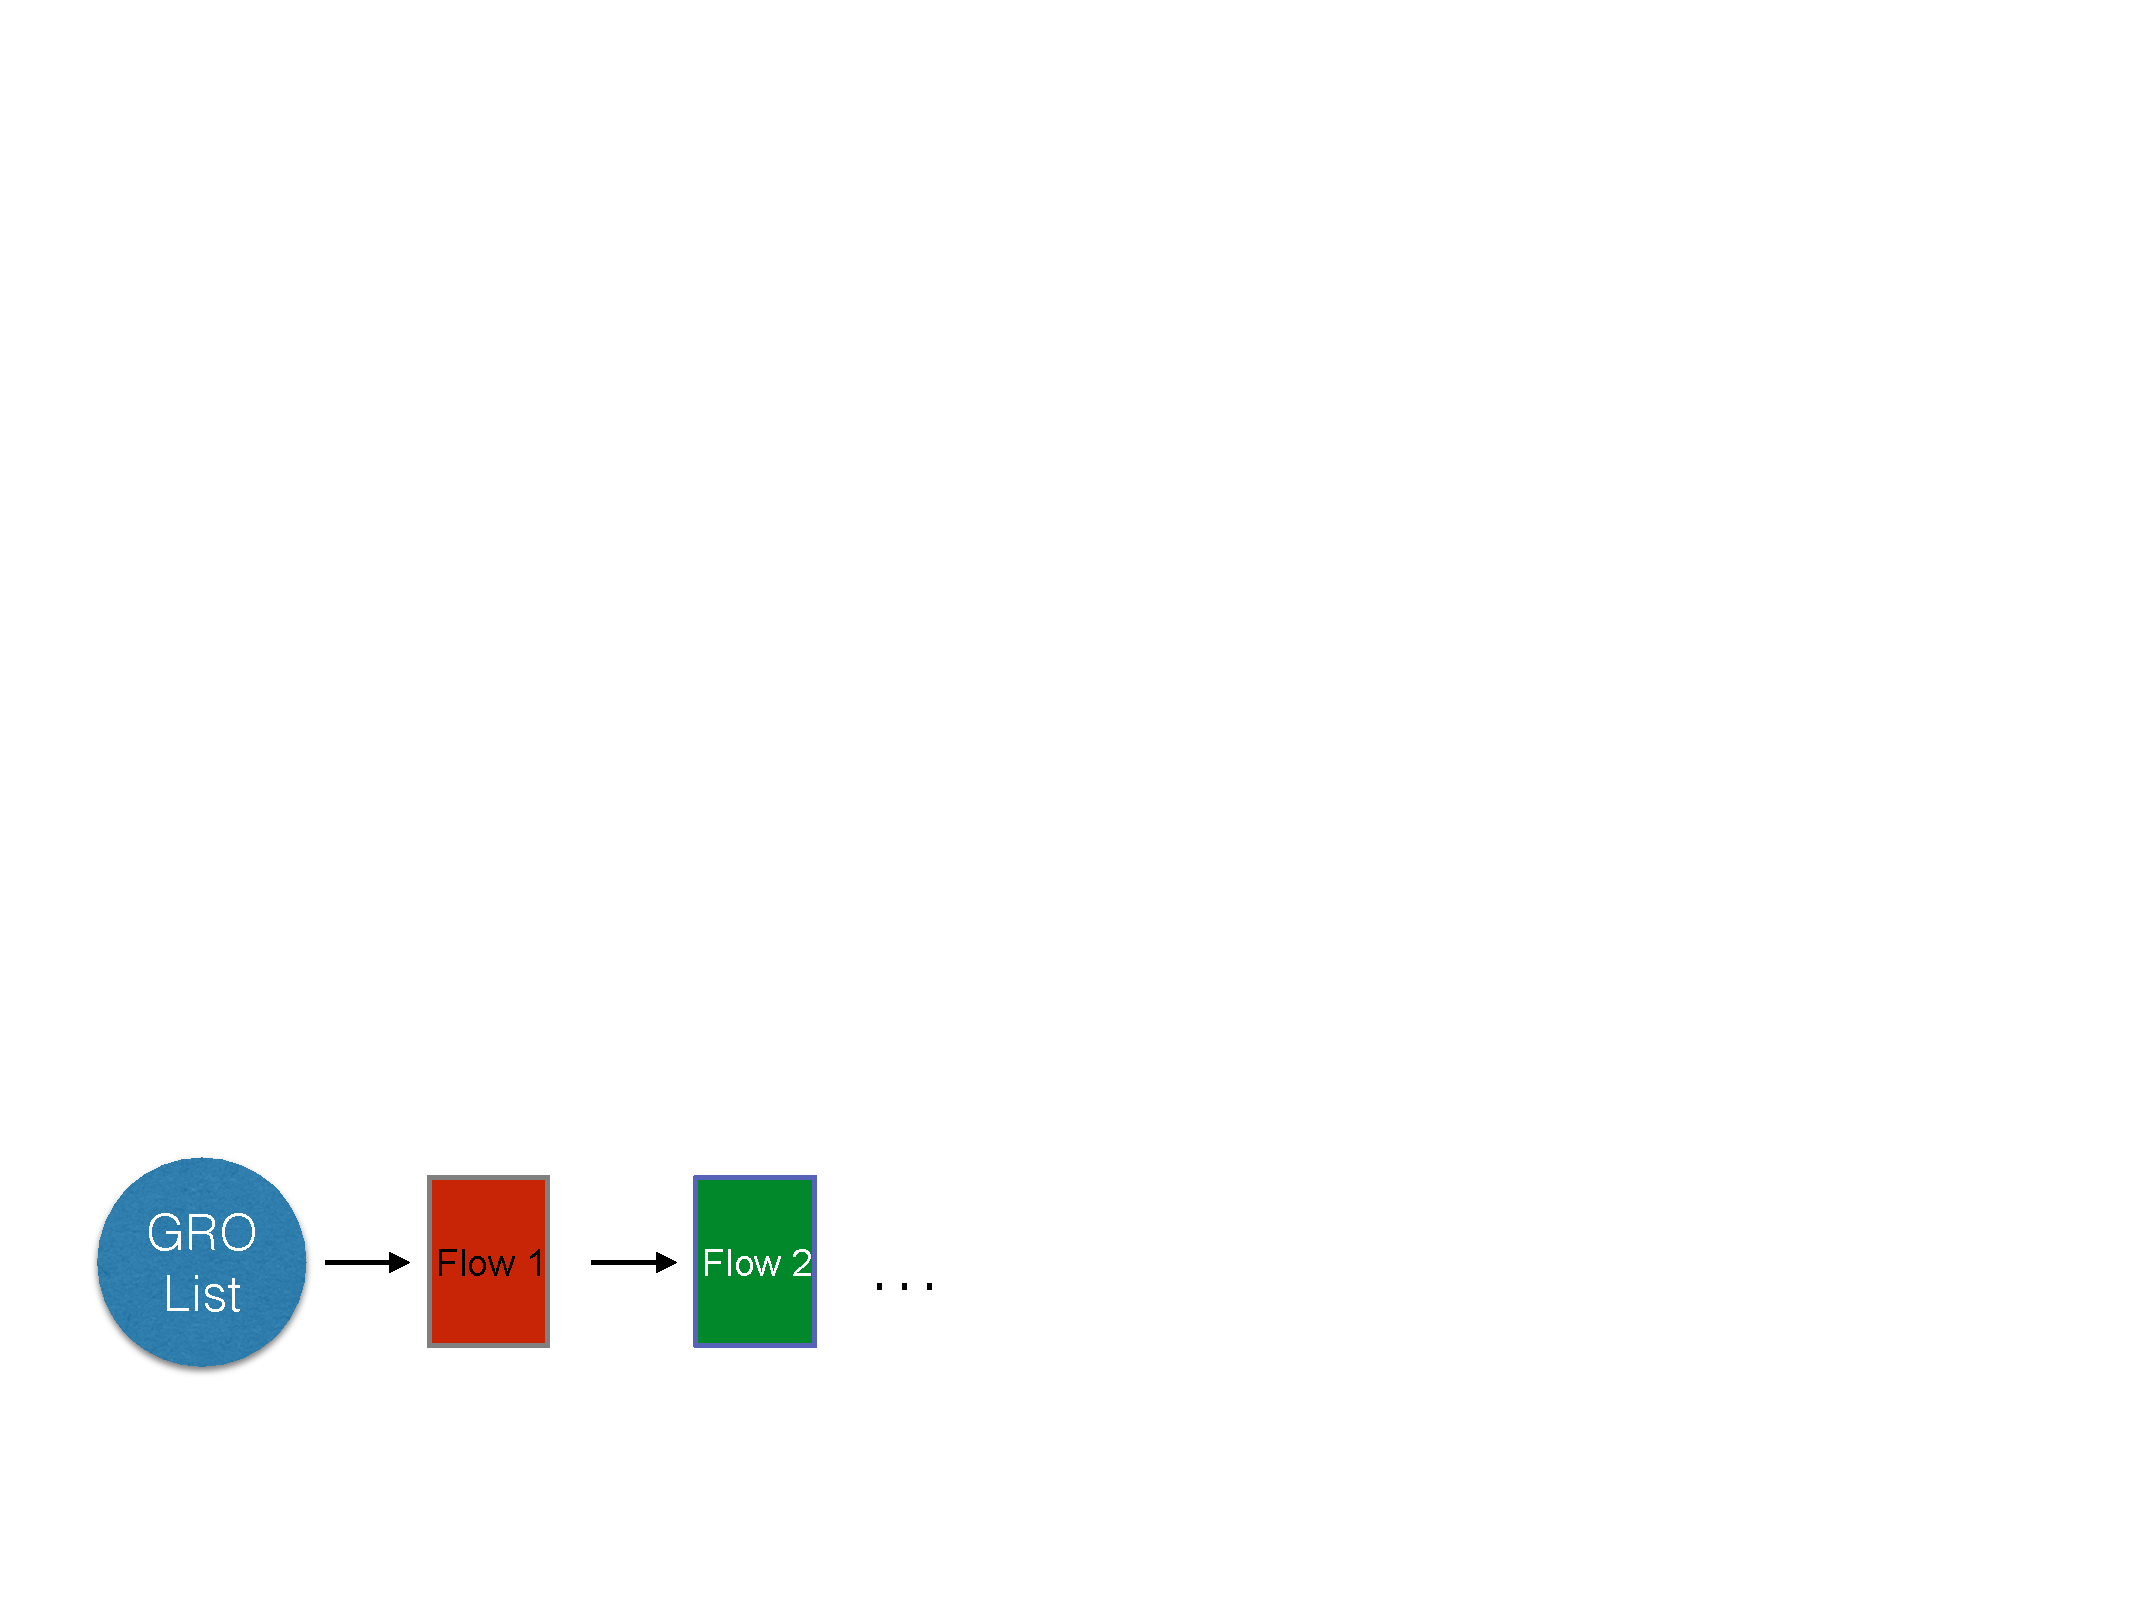
\includegraphics[width=0.45\textwidth]{presto/figures/gro-design/gro.pdf}
%        \caption{GRO design. FIX ME!}
%        \label{gro-design}
%\end{figure}

\begin{figure}[t]
        \centering
  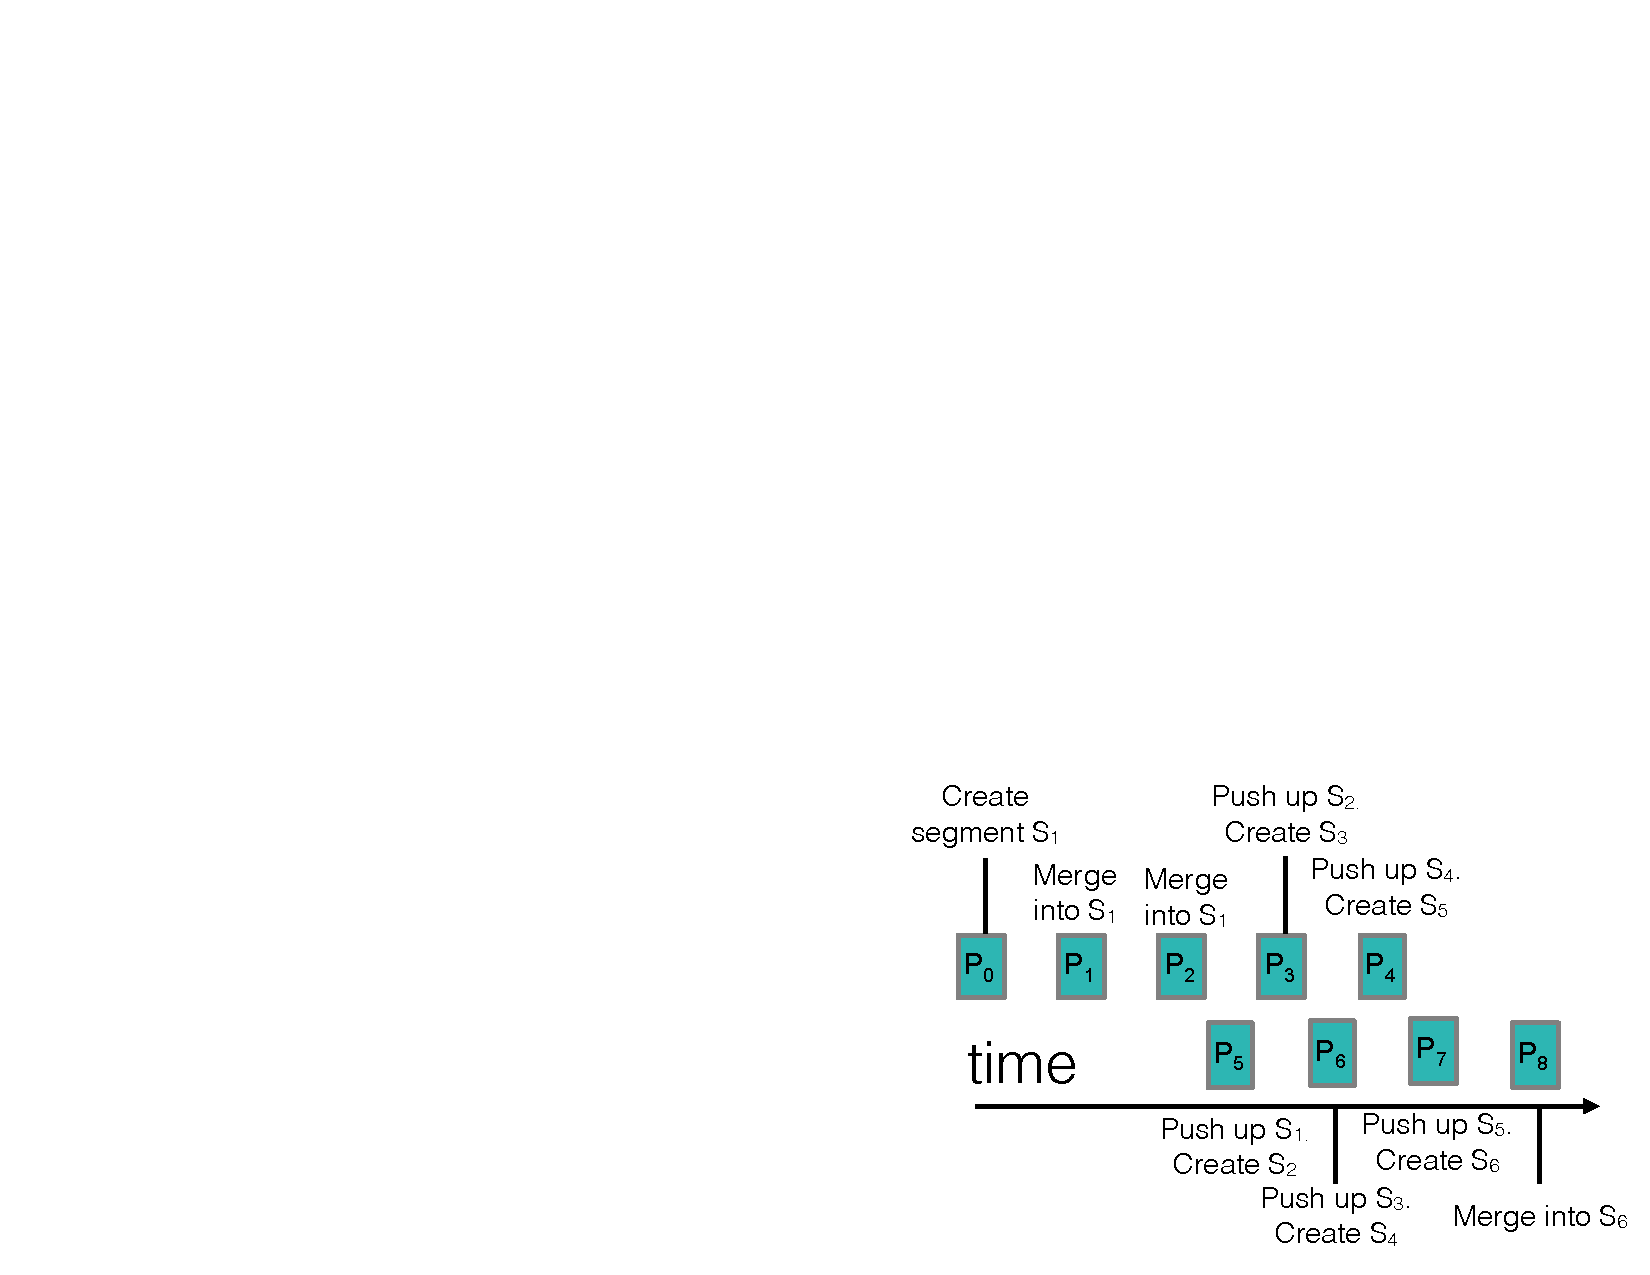
\includegraphics[width=0.45\textwidth]{presto/figures/gro-design/gro-break.pdf}
        \caption{GRO pushes up small segments ($S_i$) during reordering.}
        \label{gro-break}
\end{figure}


We now uncover how GRO breaks down in the face of reordering. Figure~\ref{gro-break} shows the impact of reordering on GRO.  Reordering does not allow the segment to grow: each reordered packet cannot be merged with the existing segment, and thus the previously created segment must be pushed up. With extreme reordering, GRO is effectively disabled because small MTU-sized segments are constantly pushed up. This causes (i) severe computational overhead and (ii) TCP to be exposed to significant amounts of reordering. We term this the {\em small segment flooding} problem.

Determining where to combat the reordering problem has not previously taken the small segment flooding problem into account.  Using a reordering buffer to deal with reordered packets is a common solution (\eg{}, works like~\cite{drb} re-sort out-of-order packets in a shim layer below TCP), but a buffer implemented above GRO cannot prevent small segment flooding.  Implementing a buffer below GRO means that the NIC must be changed, which is (i) expensive and cumbersome to update and (ii) unlikely to help combat reordering over multiple interrupts.

In our system, the buffer is implemented in the GRO layer itself.  We argue this is a natural location because GRO can
directly control segment sizes while simultaneously limiting the impact of reordering. 
Furthermore, GRO can still be applied on packets pushed up from LRO, which means hardware doesn't have to be modified
or made complex.
Implementing a better GRO algorithm has multiple challenges. The algorithm should be light-weight to scale to fast networking speeds. Furthermore, an ideal scheme should be able to distinguish loss from reordering.  When a gap in sequence numbers is detected (\eg{}, when $P_5$ is received after $P_2$ in Figure~\ref{gro-break}), it is not obvious if this gap is caused from loss or reordering.  If the gap is due to reordering, GRO should not push segments up in order to try to wait to receive the missing gap and merge the missing packets into a preestablished segment.  If the gap is due to loss, however, then GRO should immediately push up the segments to allow TCP to react to the loss as fast as possible. Ideally, an updated GRO algorithm should ensure TCP does not perform any worse than a scheme with no reordering. Finally, the scheme should adapt to prevailing network conditions, traffic patterns and application demands.




\section{Design}
\label{sec:design}

This section presents the design of Presto by detailing
the sender, the receiver, and how the network
adapts in the case of failures and asymmetry.


%\keqiang{I put datacenter load balancing goals here, TODO: need to fix the flow later}
%
%We list the design goals of datacenter load balancing:
%\begin{enumerate}
%
%\item near-perfect traffic load balancing, uniform throughput, reduced latency (or Flow completion time), minimal packet drop rate and improved fairness, regardless of flow size
%
%\item build datacenter networks on simple, unmodified commercial Ethernet switches (versus Conga)
%
%\item traffic pattern independent load balancing (versus Conga)
%
%\item less complexity and easier to deploy, using industry proven transport layer, no modification on TCP (versus MPTCP)
%
%\item support high speed data transfer (10G or 40G+) (versus packet spraying)
%
%\item resilient to hardware or link failures, adaptive to network asymmetry (versus ECMP)
%\item support varied network topologies including: flat L2 network, L3 network or L3 Networks with L2oL3 Overlays.
%L2oL3 overlays provide both L2 adjacencies and multi-tenancy scale. Trival flat L2 network provides L2 adjacencies but not multi-tenancy scale.
%Flat L2 network with shadow MAC can prodive both L2 adjacencies and multi-tenancy scale with less configuration and management overhead.
%(On Trident II chipset based switches~\cite{trident2,smart-table,arista,cisco-nexus9000}, for 8-way multipathing, L2 network with shadow MAC scale up to 35,000 physical hosts, implying half a million VMs)
%Both L2oL3 and Flat L2 network with shadow MAC support end-host virtualization and support abtraily mapping of service and physical resources
%\end{enumerate}

%%%%%macro test - test topology, 2-tier Clos network with 8 switches and 16 hosts
\begin{figure}[!t]
        \centering
  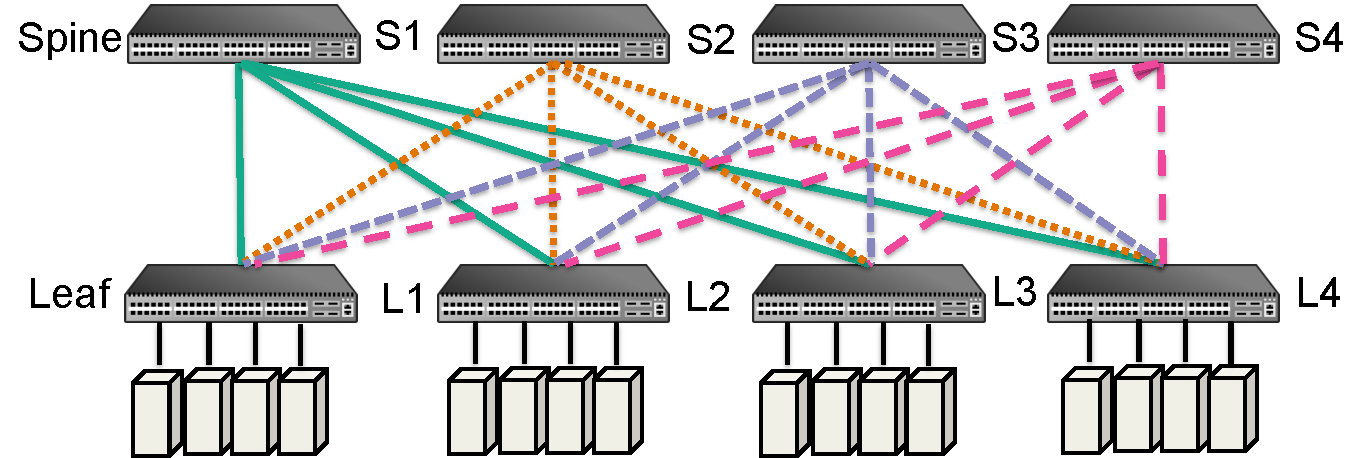
\includegraphics[width=0.5\textwidth,height=0.17\textwidth]{presto/figures/macro/macro_evaluation_topology_refined.pdf}
        \caption{Our testbed: 2-tier Clos network with 16 hosts.}
        \label{macro_evaluation_topology}
\end{figure}

\subsection{Sender}


\tightparagraph{Global Load Balancing at the Network Edge}
%controller allocation of paths
%installation of paths into OVS
%shadowMACs
In Presto, a centralized controller is employed to collect the
network topology and disseminate corresponding load balancing information to the edge vSwitches. 
The goal of this design is to ensure the vSwitches, as a whole, can load balance the network
in an even fashion, but without requiring an individual vSwitch to have detailed information
about the network topology, updated traffic matrices or strict coordination amongst senders.
 At a high level, the controller partitions
the network into a set of multiple spanning trees. Then, the controller
assigns each vSwitch a unique forwarding label in each spanning tree.
By having the vSwitches partition traffic over these spanning trees in a fine-grained
manner, the network can load balance traffic in a near-optimal fashion.

%We extend previous work that creates per-destination spanning trees in the network,~\ie PAST~\cite{past},
%by computing multiple disjoint spanning trees for every destination.
The process of creating spanning trees is made simple by employing multi-stage Clos
networks commonly found in datacenters. For example, in a 2-tier Clos network
with $\nu$ spine switches, the controller can easily allocate $\nu$ disjoint spanning
trees by having each spanning tree route through a unique spine switch. Figure~\ref{macro_evaluation_topology}
shows an example with four spine switches and four corresponding disjoint spanning trees.
When there are $\gamma$ links between each spine and leaf switch in a 2-tier Clos network,
the controller can allocate $\gamma$ spanning trees per spine switch.
Note that 2-tier Clos networks cover the overwhelming 
majority of enterprise datacenter deployments and can
support tens of thousands of physical servers~\cite{conga}.
%are scalable because they easily support a large number
%of hosts with only a few high density spine switches~\cite{conga}.
The controller ensures links in the network are equally covered
by the allocated spanning trees.
%~\keqiang{An example (similar to CONGA's example to convince people that 2-tier spine-leaf architecture is enough for most deployments).
%Let's use leaf switches with 48 10G ports and 12 40G uplinks. Combined with spine switches with 100s of 40G ports, 
%an non-oversubscribed 2-ter spine-leaf network which supports 20,000+ 10G nodes can be built. 
%In such a network, each 10G server can have 12 shadow MACs (there are only 12 disjoint spanning trees in the network)}

Once the spanning trees are created, the controller assigns a unique forwarding label
for each vSwitch in every spanning tree and installs the relevant forwarding rules into the network.
Forwarding labels can be implemented in a variety of ways using
technologies commonly deployed to forward on labels,
such as MPLS~\cite{casado2012fabric}, VXLAN~\cite{conga,nv-mtd}, or IP encapsulation~\cite{drb}. 
In Presto,
label switching is implemented with shadow MACs~\cite{shadow-mac}. 
Shadow MACs implement label-switching for commodity Ethernet by using the 
destination MAC address as an opaque forwarding label that can easily be 
installed in L2 tables. 
Each vSwitch is assigned one shadow MAC per spanning tree.
Note Shadow MACs are extremely scalable on
existing chipsets because they utilize the large L2 forwarding table. For example,
Trident II-based switches~\cite{trident2,smart-table,arista} have 288k L2 table entries and 
thus 8-way multipathing (\ie{}, each vSwitch has 8 disjoint spanning trees)
can scale up to 36,000 physical servers. 
%\textcolor{blue}{which covers an overwhelming fraction of enterprise deployments~\cite{conga}.
To increase scalability, shadow MAC tunnels can be implemented from 
edge switch to edge switch instead of from vSwitch to vSwitch. Switch-to-switch
tunneling has been proposed in previous works such as MOOSE~\cite{moose} and NetLord~\cite{netlord}. 
Tunneling requires $\mathcal{O}(|switches|\times|paths|)$ rules instead of
$\mathcal{O}(|vSwitches|\times|paths|)$ rules. All 
shadow MAC labels can route to a destination 
edge switch that forwards the packet to the correct destination by forwarding on 
L3 information.

Finally, we note that shadow MACs are also compatible with network virtualization 
(both L2 and L3 address space virtualization). 
Tunneling techniques such as VXLAN encapsulate packets in Ethernet frames, 
which means shadow MACs should still allow path selection 
in virtualized environments by modifying outer Ethernet headers.
VXLAN hardware offload is supported in modern NICs and has little
performance overhead~\cite{vxlan-bench}.
%\eric{cite?}~\keqiang{CONGA says 20000+ is okay for an overwhelming fraction of enterprise deployments, seems to be true 
%after reading fat-tree and some googling}

%Shadow MACs allow for fine-grained, dynamic
%and consistent control of the forwarding tables in the network, but without using TCAM tables. Instead, shadow MACs use the destination MAC address
%as an opaque forwarding label in the network. Each shadow MAC can correspond to a destination-based tree. Then, the controller can preinstall
%these trees into the network. In OVS, the Presto module can use the destination IP address into a lookup table, with the entries corresponding
%to distinct paths for each destination. The OVS agent rewrites the destination MAC address to the corresponding shadow MAC address, and the Presto
%agent running on the receiver will rewrite the shadow MAC back to the original MAC address. (ugh, clean this up!). The OVS agent rewrites the destination
%MAC address of the TSO segment, and this segment is pushed to the NIC. The NIC then creates MTU-sized packets from this segment, with each packet having
%the shadow MAC address.
%
%A user space module accepts destination to multiple path mappings from the controller. Upon
%receiving a flow for the first time, the kernel module in OVS queries the user level module. If the flow is found, the path mappings are
%pushed into the kernel module. If not, the controller is queried for the destination information. OVS keeps state of the ongoing flow, and
%modifies the incoming packets with routing information for path selection as needed on a sub-flow level.



\tightparagraph{Load Balancing at the Sender}
%TSO/cell is a natural marriage
%round-robin over cells to load-balance over network
%rewrite dest MAC address to shadow MAC
% MTU size change is bad?
%chunkID insertion into packet
%make clear this is all done in OVS: blurb or two about advantages
\begin{algorithm}[t]
\caption{Pseudo-code of flowcell creation}
\label{alg:flowcell}
\begin{algorithmic}[1]
\IF{bytecount + len(skb) $>$ {\emph {threshold}}}
\STATE bytecount $\leftarrow$ len(skb)
\STATE current\_mac $\leftarrow$ (current\_mac + 1) \% {\emph {total\_macs}}
\STATE flowcellID $\leftarrow$ flowcellID + 1
\ELSE
\STATE bytecount $\leftarrow$ bytecount + len(skb)
\ENDIF
\STATE skb $\leftarrow$ update(skb, current\_mac, flowcellID)
\STATE sendToNIC(skb)
\end{algorithmic}
\end{algorithm}
After the controller installs the shadow MAC forwarding rules into the network, it creates a mapping
from each physical destination MAC address to a list of corresponding shadow MAC addresses. These mappings
provide a way to send traffic to a specific destination over different spanning trees. 
The mappings are pushed from the controller to each vSwitch in the network, either on-demand or preemptively.
In Presto, the vSwitch on the sender monitors outgoing traffic (\ie{}, maintains a per-flow counter in the datapath) 
and rewrites the destination MAC
address with one of the corresponding shadow MAC addresses.
The vSwitch assigns the same shadow MAC address to all consecutive segments until the 64 KB limit is reached.
In order to load balance the network effectively, the vSwitch 
iterates through destination shadow MAC addresses in a round-robin fashion. 
This allows the edge vSwitch to load balance over the network in a very fine-grained fashion.
%\eric{we have to decide where to formally define correct algorthm for chunk. that is, we don't
%load balance on TSO segments exactly, because if multiple consectutive TSO segments arrive whose sum
%is < 64 KB, then we will assign them all to the same chunk ID. this helps with small flows that consist
%of many segments, but whose sums are less than 64 KB.}
%When the first segment of a flow arrives, the vSwitch randomly chooses the a shadow MAC from
%the list and then subsequentially assigns shadow MACs to segments in a round robin fashion.

Sending each 64 KB worth of flowcells over a different path in the network can cause reordering and must
be carefully addressed.
To assist with reordering at the receiver (Presto's mechanisms for combatting reordering are detailed in the next section), 
the sender also includes a sequentially increasing {\em flowcell ID} into each segment.
%For example, 
In our setup the controller installs forwarding rules solely on the destination MAC address and
ARP is handled in a centralized manner. Therefore,
the source MAC address can be used to hold the flowcell ID. Other options are possible, 
\eg{}, some schemes include load balancing metadata in the reserved bits of the VXLAN header~\cite{nvo3}
and implementations could also stash flowcell IDs into large IPv6 header fields.\footnote{In our
implementation, TCP options hold the flowcell ID for simplicity and ease of debugging.}
Note that since the flowcell ID and the shadow MAC address are modified before a segment is handed to the NIC,
the TSO algorithm in the NIC replicates these values to all derived MTU-sized packets.
The pseudo-code of flowcell creation is presented in Algorithm~\ref{alg:flowcell}.
Since this code executes in the vSwitch, retransmitted TCP packets run through this code for each retransmission.

\begin{algorithm}[!t]
\caption{Pseudo-code of Presto GRO {\tt flush} function}
\label{alg:gro}
\begin{algorithmic}[1]
%\REQUIRE $n \geq 0 \vee x \neq 0$
%\ENSURE $y = x^n$
\FOR{each flow f}
\FOR{$S \in f.{\tt segment\_list}$}
%\STATE f = getFlow(S)
\IF{f.lastFlowcell == getFlowcell(S)}
\STATE f.expSeq $\leftarrow$ max(f.expSeq, S.endSeq)
\STATE pushUp(S)
\ELSIF{getFlowcell(S) $>$ f.lastFlowcell}
\IF{f.expSeq == S.startSeq}
\STATE f.lastFlowcell $\leftarrow$ getFlowcell(S)
\STATE f.expSeq $\leftarrow$ S.endSeq
\STATE pushUp(S)
\ELSIF{f.expSeq > S.startSeq}
\STATE f.lastFlowcell $\leftarrow$ getFlowcell(S)
\STATE pushUp(S)
\ELSIF{timeout(S)}
\STATE f.lastFlowcell $\leftarrow$ getFlowcell(S)
\STATE f.expSeq $\leftarrow$ S.endSeq
\STATE pushUp(S)
\ENDIF
\ELSE
\STATE pushUp(S)
\ENDIF
\ENDFOR
\ENDFOR
\end{algorithmic}
\end{algorithm}

\subsection{Receiver}
The main challenge at the receiver is dealing with reordering that can occur when different flowcells
are sent over different paths. The high-level goal of our receiver implementation is
to mitigate the effects of the small segment flooding problem by (i) not so aggressively pushing
up segments if they cannot be merged with an incoming packet and (ii) ensuring that segments
pushed up are delivered in-order.

\tightparagraph{Mitigating Small Segment Flooding} Let's use Figure~\ref{gro-break} as a motivating example 
on how to combat the small segment flooding problem. Say a polling event has occurred, and the driver retrieves
9 packets from the NIC ($P_0$-$P_8$). The driver calls the GRO handler, which merges consecutive packets
into larger segments. The first three packets ($P_0$-$P_2$) are merged into a segment, call it $S_1$ (note: in practice
$S_1$ already contains in-order packets received before $P_0$).
When $P_5$ arrives, a new segment $S_2$, containing $P_5$, should be created. Instead of pushing up $S_1$ (as is done currently),
both segments should be kept.
Then, when $P_3$ is received, it can be merged into $S_1$. Similarly, $P_6$ can be merged into $S_2$. This process
can continue until $P_4$ is merged into $S_1$. At this point, the gap between the original out-of-order reception ($P_2$-$P_5$)
 has been filled, and $S_1$ can be pushed up and $S_2$ can continue to grow. This means the size of the segments being pushed up is increased,
and TCP is not exposed to reordering.

The current default GRO algorithm works as follows. An interrupt by the NIC causes the driver to poll
(multiple) packets from the NIC's ring buffer. The driver calls the GRO handler on the received batch
of packets. GRO keeps a simple doubly linked list, called {\tt gro\_list}, that contains 
segments, with a flow having at most one segment in the list. When packets for a flow are
received in-order, each packet can be merged into the flow's preexisting segment. When a packet
cannot be merged, such as with reordering, the corresponding segment is pushed up (ejected from the
linked list and pushed up the networking stack) and a new segment is created from the packet. 
This process is continued until all packets in the batch are serviced. At the end 
of the polling event, a {\tt flush} function is called that pushes up all segments in the
{\tt gro\_list}.
% that are not "too new" (\ie{}, segments that were just created near the end of the polling
%event and haven't had many packets merged into them).

Our GRO algorithm makes the following changes. First, multiple segments can be
kept per flow in a doubly linked list (called {\tt segment\_list}). 
To ensure the merging process is fast, each linked list is kept in a hash table (keyed on flow).
When an incoming packet cannot be merged with any existing segment, the existing
segments are kept and a new segment is created from the packet.
New segments are added to the head of the linked list so that merging subsequent packets is typically $\mathcal{O}(1)$.
When the merging is completed over all packets in the batch, the {\tt flush} function is called. 
The {\tt flush} function decides whether to push segments up or to keep them. Segments may 
be kept so reordered packets still in flight have enough time to arrive and can then be placed in-order
before being pushed up. 
Reordering can cause the linked lists to become slightly out-of-order, so
at the beginning of {\tt flush} an insertion sort is run to help easily decide if segments are in-order.
%\eric{this is likely too long and too repetitive with section 2. keqiang, please go over to check for
%correctness. we need to figure out the write level of detail to go into here. we also need
%to say what the impact of using sMACs is here... how are flows decided? i'm also missing
%other pushUp events: like max segment size being reached, timeout occuring on segment, etc.}

The pseudo-code of our {\tt flush} function is presented in Algorithm~\ref{alg:gro}.
For each flow, our algorithm keeps track of the next expected in-order
sequence number ({\tt f.expSeq}) and the corresponding flowcell ID
of the most recently received in-order sequence number ({\tt f.lastFlowcell}).
When the merging is completed, the {\tt flush} function iterates over 
the sorted segments ($S$), from lowest sequence number to highest sequence number in the {\tt segment\_list} (line 2).
The rest of the code is presented in the subsections that follow.


\tightparagraph{How to Differentiate Loss from Reordering?} 
In the case of no loss or reordering, our algorithm keeps pushing up segments and updating state. Lines 3-5
deal with segments from the same flowcell ID, so we just need to update {\tt f.expSeq} each time. Lines 
6-10 represent the case when the current flowcell ID is fully received and we start to receive the
next flowcell ID.
The problem, however, is when there is 
a gap that appears between the sequence numbers of the segments. When a gap is encountered,
it isn't clear if it is caused from reordering or from loss. If the gap is due to reordering,
our algorithm should be conservative and try to wait to receive the packets that "fill in the gap" 
before pushing segments up to TCP. If the gap is due to loss, however, then we should push up the 
segments immediately so that TCP can react to the loss as quickly as possible.

%We solve this seemingly difficult problem in a simple fashion. 
%Since chunk sizes are small and 
%all packets within a chunk are routed on the same shadow MAC address, it is highly likely all packets
%within the same chunk will traverse the same network path
To solve this problem, we leverage the fact that all packets carrying the same flowcell ID traverse the 
same path and should be in-order.
This means incoming sequence numbers can be monitored to check for
gaps. A sequence number gap within the same flowcell ID is assumed to be a loss, and not reordering,
so those packets are pushed up immediately (lines 3-5).
Note that because a flowcell consists of many packets (a 64 KB flowcell consists
of roughly 42 1500 byte packets), when there is a loss it is likely that it occurs within flowcell boundaries. 
The corner case, when a gap occurs on the flowcell boundary, leads us to the next design question.

\tightparagraph{How to Handle Gaps at Flowcell Boundaries?}
When a gap is detected in sequence numbers at flowcell boundaries, it is not clear if the gap is due
to loss or reordering. Therefore, the segment should be held long enough to
handle reasonable amounts of reordering, but not so long that TCP cannot respond
to loss promptly. Previous approaches that deal with reordering typically employ a large static
timeout (10ms)~\cite{drb}. 
Setting the timeout artificially high can handle reordering, but hinders TCP when the gap is
due to loss. 
Setting a low timeout is difficult because many dynamic factors, such as delays between
segments at the sender, network congestion, and traffic patterns (multiple flows 
received at the same NIC affect inter-arrival time), can cause large variations.
%XXXERICLEFTHERE
%because there are often many causes for variations in delay: 
%the sender (senders often have delays between segments), the network (different
%queue lengths from congestion over different paths), and the traffic patterns (multiple flows received at the same NIC affect
%inter-arrival time). 
%As a result, we devised an adaptive timeout to help deal with dynamic variations. 
As a result, we devise an adaptive timeout scheme, which monitors recent reordering events and sets a dynamic timeout value accordingly.
Presto tracks cases when there is reordering, but no loss, on flowcell boundaries and keeps an exponentially-weighted
moving average ($EWMA$) over these times. Presto then applies a timeout of $\alpha * EWMA$ to a segment when a gap is 
detected on flowcell boundaries. 
Here $\alpha$ is an empirical parameter that allows for timeouts to grow. As a further optimization, if a segment
has timed out, but a packet has been merged into that segment in the last $\frac{1}{\beta} * EWMA$ time interval, then 
the segment is still held in hopes of preventing reordering. We find $\alpha$ and $\beta$
work over a wide range of parameters and set both of them to 2 in our experiments. A timeout firing is dealt with in lines 14-18.
%\eric{take out GRO\_LIST.full()?}


%\textcolor{blue}{
\tightparagraph{How to Handle Retransmissions?} Retransmitted TCP packets are pushed up immediately in order to allow the TCP stack to react without delay. 
If the flowcell ID of the retransmission is the same as the expected flowcell ID, then 
the retransmission will be pushed up immediately because its sequence number will be $\leq f.expSeq$. 
If the flowcell ID is larger
than the expected flowcell ID (when the first packet of a flowcell is a retransmission), then the packet is pushed up (line 13). 
If a retransmitted packet has a smaller flowcell ID than the next expected flowcell ID (a stale packet),
then it will be pushed up immediately (line 20). 
Note we ensure overflow is handled properly in all cases.


%\tightparagraph{How to handle shadow MACs with OVS?}
%~\keqiang{Can we take this paragraph out, just feel that it breaks the flow of this paper}
%OVS has many optimizations to handle segments at line rate. One problem with using shadow MACs is that many keys 
%may be created for the same flow (since OVS hashes on MAC addresses).
%At the receiver, we overwrite the destination MAC address to the physical MAC address and overwrite the source MAC 
%address to a consistent dummy value\footnote{The controller handles all ARP messages in Presto} before any lookups. At the sender,
%we do not overwrite any MAC address until after the table lookup.
%Rewriting the MAC address also makes any of our changes completly transparent to higher layers in the networking
%stack.
%\eric{move to discussion?}

%We found OVS makes a few assumptions in which our code caused issues. The default implementation of OVS does a flow
%lookup in which it uses hashed header values as a key. The key hashes on ethernet addresses, and the first time a packet is received
%for this tuple, OVS must do a lookup into user level. In the implementation, the first packet received is pushed to user
%level, but the packet size is bound to 1500 bytes. This means if a large packet is received as the first packet on a key,
%then OVS must break the large packet into 1500 byte packets and pushes them {\em all} to user space. Normally, this is not a problem,
%because the SYN packet is a first packet of a flow, so (i) it is small and (ii) the round-trip time of TCP's handshake gives
%the user level calls time to complete. In Presto however, the SYN packet may not share the same ethernet destination as subsequent
%data packets. This means that a large data packet can be the first packet to arrive over a given ethernet destination. This
%originally caused substainal packet reordering and much overhead at the beginning of a TCP connection in Presto. We were able
%to simply fix the problem by writing the shadow MAC address back to the original destination MAC address before any key lookups
%in OVS. Rewriting the shadow MAC address also makes any of our changes completly transparent to higher layers in the networking
%stack.

%\eric{should we talk about using a path ID instead of a chunk ID? then don't have to change anything but shadowMAC. this 
%is only doable if the receiver knows the round-robin scheduling that the sender is employing. should we also talk
%about using something like source port to get ECMP to hash onto different paths? this is done by MPTCP and the 
%vmware blog}


\subsection{Failure Handling and Asymmetry}
%Monthly switch and link availability have been 
%shown to be 99.99\% and 99.95\%, respectively~\cite{wcmp}.
When failures occur, Presto relies on the controller to update the forwarding
behavior of the affected vSwitches. The controller can simply prune the spanning
trees that are affected by the failure, or more generally enforce a weighted
scheduling algorithm over the spanning trees.
Weighting allows for Presto to evenly distribute traffic over an asymmetric topology.
Path weights can be implemented in a simple fashion by duplicating shadow MACs used in
the vSwitch's round robin scheduling algorithm.
For example, assume we have three paths in total ($p_1$, $p_2$ and $p_3$) and their updated weights are 0.25, 0.5 and 0.25 respectively.
Then the controller can send the sequence of $p_1$, $p_2$, $p_3$, $p_2$ to the vSwitch, which
can then schedule traffic over this sequence in a round robin fashion to realize the new path weights.
This way of approximating path weights in the face of network
asymmetry is similar to WCMP~\cite{wcmp}, but instead of having to change switch firmware and use
scarce on-chip SRAM/TCAM entries, we can push the weighted load balancing entirely to the network edge.

As an added optimization, Presto can leverage any fast failover features that 
the network supports, such as BGP fast external failover, MPLS fast reroute, or OpenFlow failover groups. Fast failover detects port failure and can move corresponding traffic
to a predetermined backup port. Hardware failover latency ranges from several to tens of milliseconds~\cite{ipblog-failover,huawei-failover}.
This ensures traffic is moved away from the failure rapidly and the network
remains connected when redundant links are available.
% and contains redundant links~\keqiang{like Facebook's "protection ring"~\cite{farrington2013facebook}}. 
Moving to backup links causes imbalance in the network,
so Presto relies on the controller learning of the network change, computing weighted multipath schedules, and
disseminating the schedules to the edge vSwitches. 

%\subsection{Non-SDN Environments}
%Instead of using shadow MACs, Presto can be implemented in non-SDN environments in the following manner. First,
%the approach must rely on ECMP in the fabric. ECMP can be configured to hash on a wide variety of network headers (cite).
%As done in MPTCP, and mentioned in online discussions, the Layer 4 source port can be varied to force ECMP to 
%route different sub-flows onto different paths. In Presto, the chunk ID can easily be stashed in the TCP source
%port. HOW DOES THE RECEIVER DEAL WITH THIS? (must not break RSS, must allow receiver to echo packets back to sender, etc). 

%
% old stuff.
%
%PAST~\cite{past}.
%Open vSwitch has been acting as the intelligent {\em network edge} in datacenter networks~\cite{ovs-extending,ovs-edge,nv-mtd}.
%TCP offload~\cite{tcp-offload,optimize-tcp-receive}.
%Generic Receive Offload (GRO)~\cite{gro,bullettrains}.
%New API (NAPI)~\cite{understanding-linux-network}.
%Link/switch failures in datacenters~\cite{dc-failures,wcmp}.

\section{Methodology}
\label{sec:method}

\tightparagraph{Implementation}
We implemented Presto in Open vSwitch v2.1.2~\cite{ovs-website} and Linux kernel v3.11.0~\cite{kernel}.
In OVS, we modified 5 files and $\sim$600 lines of code. For GRO, we modified 11 files and $\sim$900 lines of code.
%The GRO handler in Presto is implemented in the kernel (in directory {\tt /net/core/})
%, but there have been discussions
%of moving the GRO handling code into network drivers or to a loadable kernel module. (cite XXX). 
%eric-- the reference above is from 2009, so i think we'll skip this

%other sections probably talk about what we did
%Presto uses chunk size of 32KB/25.6$\mu\text{s}$ (used in combination with TCP small queue~\cite{tsq} which is used for
%reducing latencies on network stack) or 
%64KB/51.2$\mu\text{s}$ (default TCP segment offload size) for 10GbE.



%\subsection{Methodology} 
\tightparagraph{Testbed} We conducted our experiments on a physical
testbed consisting of 16 IBM System x3620 M3 servers with 6-core Intel Xeon
2.53GHz CPUs, 60GB memory, and Mellanox ConnectX-2 EN 10GbE NICs. 
The servers were connected in a 2-tier Clos network topology with 10 Gbps
IBM RackSwitch G8264 switches, as shown in Figure~\ref{macro_evaluation_topology}.

\tightparagraph{Experiment Settings}
We ran the default TCP implementation in the Linux kernel (TCP CUBIC~\cite{cubic})
%3.11.0 and uses MPTCP version 0.88~\cite{mptcp-linux}.
%We use default TSO size 64KB
and set parameters {\tt tcp\_sack}, {\tt tcp\_fack}, {\tt tcp\_low\_latency} to 1. 
Further, we tuned the host Receive Side Scaling (RSS)~\cite{rss} and IRQ affinity settings and kept them the same in all experiments.
We send and receive packets from the hypervisor OS instead of VMs. 
LRO is not enabled on our NICs.
%For MPTCP, we set the subflow count to 8, use OLIA congestion control algorithm~\cite{mptcp-not-optimal}, and configure buffer sizes
%as recommended by ~\cite{dc-mptcp,mptcp-not-optimal,paasch2013benefits}.

\tightparagraph{Workloads}
We evaluate Presto with a set of synthetic and realistic workloads. 
Similar to previous works~\cite{fattree,hedera,planck}, our synthetic workloads include:
{\em Shuffle}: Each server in the testbed sends 1GB data to every other server in the testbed in random order. 
Each host sends two flows at a time. %The shuffle is finished if all the servers have finished their jobs. 
This workload emulates the shuffle behavior of Hadoop workloads.
{\em Stride(8)}: We index the servers in the testbed from left to right. In stride(8) workload, server[i] sends to server[(i+8) mod 16].
{\em Random}: Each server sends to a random destination 
 not in the same pod as itself. Multiple senders can send to the same receiver.
{\em Random Bijection}: Each server sends to a random destination not in the same pod as itself. 
Different from random, each server only receives data from one sender.
Finally, we also evaluate Presto with trace-driven workloads from real datacenter traffic~\cite{kandula2009nature}.

\tightparagraph{Performance Evaluation}
We compare Presto to ECMP, MPTCP, and a 
single non-blocking switch used to represent an optimal scenario.
ECMP is implemented by enumerating all possible end-to-end paths and randomly selecting a path for each flow.
MPTCP uses ECMP to determine the paths of each of its sub-flows.
%We use MPTCP version 0.88~\cite{mptcp-linux}, set the subflow count to 8, use OLIA congestion control algorithm~\cite{mptcp-not-optimal}, and configure buffer sizes
%as recommended by ~\cite{dc-mptcp,mptcp-not-optimal,paasch2013benefits}. 
The MPTCP implementation is still under active development, and
we spent significant effort in finding the most stable configuration of MPTCP on our testbed. Ultimately, we found that Mellanox {\tt mlx\_en4} driver version
2.2, MPTCP version 0.88~\cite{mptcp-linux}, subflow count set to 8, OLIA congestion control algorithm~\cite{mptcp-not-optimal}, and configured buffer sizes
as recommended by~\cite{dc-mptcp,mptcp-not-optimal,paasch2013benefits} gave us the best trade-offs in terms of throughput, latency, loss and stability.
Unfortunately, despite our efforts, we still occasionally witness some stability issues 
with MPTCP that we believe are due to implementation bugs.

We evaluate Presto on various performance metrics, including: 
throughput (measured by {\tt nuttcp}), round trip time (a single TCP packet, measured by {\tt sockperf}~\cite{sockperf}), 
mice flow completion time (time to send a 50 KB flow and receive an application-layer acknowledgement), packet loss (measured from switch counters), 
and fairness (Jain's fairness index~\cite{jain-fair} over flow throughputs).  Mice flows are sent every 100 ms and elephant flows last 10 seconds. 
Each experiment is run for 10 seconds over 20 runs. Error bars on graphs denote
the highest and lowest value over all runs.


\section{Microbenchmarks}
\label{sec:micro}

We first evaluate the effectiveness of Presto over a series of microbenchmarks. Using 
canonical topologies, we investigate (i) Presto's effectiveness in preventing the small segment
flooding problem and reordering, (ii) Presto's CPU overhead, (iii) Presto's ability to scale
to multiple paths, (iv) Presto's ability to handle congestion, (v) comparison to flowlet
switching, and (vi) comparison to local, per-hop load balancing.

%%%%%micro test - scalability and congestion test topology
\begin{figure}[t]
        \centering
	\begin{subfigure}[b]{0.225\textwidth}
        	\centering
  		\includegraphics[width=\textwidth]{./figures/micro_test_topology/micro_scalabilitytest_topology_refined.pdf}
        	\caption{}
		\label{micro_scalability_topology}
	\end{subfigure}
	\begin{subfigure}[b]{0.225\textwidth}
                \centering
		\includegraphics[width=\textwidth]{./figures/micro_test_topology/micro_congestiontest_topology_refined.pdf}
        	\caption{}
		\label{micro_congestion_topology}
	\end{subfigure}
	\caption{(a) Scalability benchmark and (b) Oversubscription benchmark topology.}
	\label{micro_topology}
\end{figure}

%%%%%gro effectiveness shows
\begin{figure}[t]
	\centering
	\begin{subfigure}[b]{0.225\textwidth}
                \centering
  		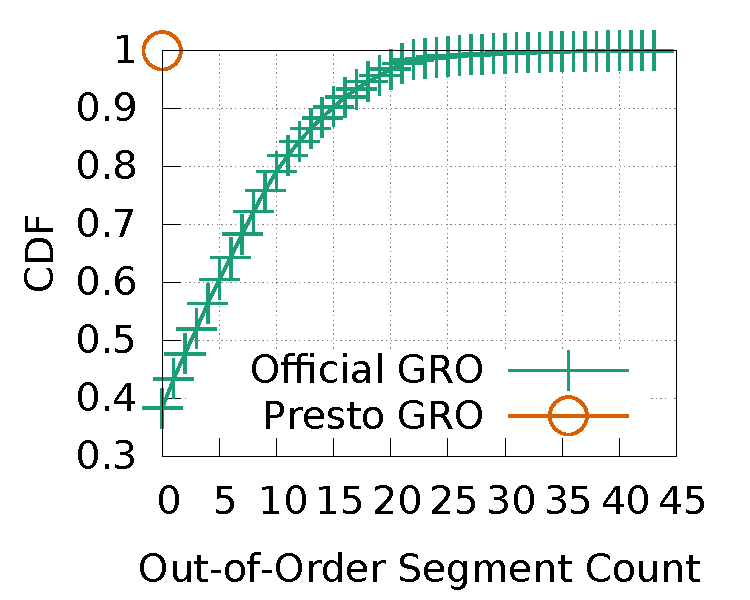
\includegraphics[width=\textwidth]{./figures/gro_effectiveness/metric1_seg_cdf_compare.pdf}
		\caption{}
		\label{gro_effectiveness_on_reordering}
	\end{subfigure}
        \begin{subfigure}[b]{0.225\textwidth}
                \centering
		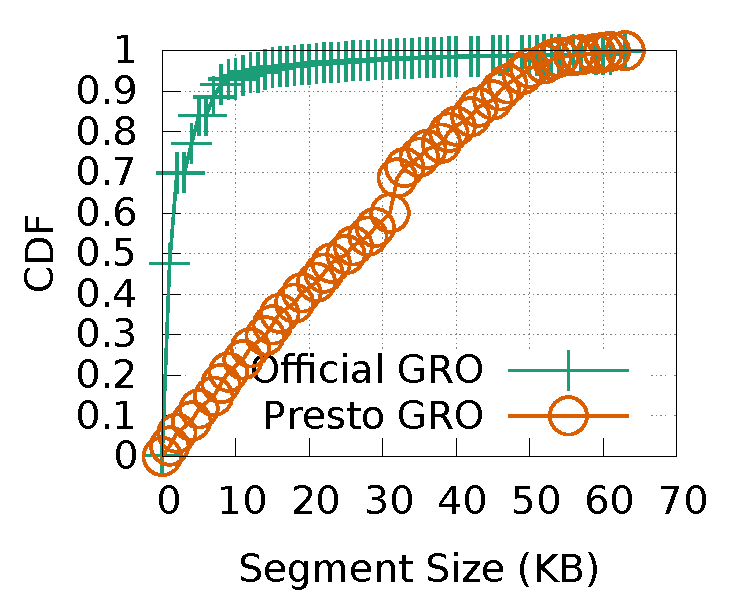
\includegraphics[width=\textwidth]{./figures/gro_effectiveness/metric1_pktsize_cdf_compare.pdf}
        	\caption{}
		\label{gro_effectiveness_on_pktsize}
	\end{subfigure}
	\caption{(a) Illustration of the modified GRO's effectiveness on masking reordering. 
		%We use the number of  segments from other chunks
                %between the first segment and last segment of each chunk
                %seen by TCP to measure the extent of packet reordering
		(b) In case of massive packet reordering, official GRO cannot merge packets effectively such that lots of small
                packets are processed by TCP which poses great processing overhead for CPU.}
	\label{gro_effectiveness}
\end{figure}

\tightparagraph{Presto's GRO Combats Reordering}
To examine Presto's ability to handle packet reordering, we perform a simple experiment
on topology shown in Figure~\ref{micro_congestion_topology}.
%we compare the extent of TCP reordering, TCP segment size distribution, throughput and receiver side CPU usage 
%using official GRO and Presto GRO. 
Here two servers attached to leaf switch L1 
send traffic to their own receivers attached to leaf switch L2
by spreading 64KB flowcells over the two network paths. 
%Because these two flows share the same two paths 
%so packet reordering can happen at the receiver side.
This setup can cause reordering for each flow, so 
we compare Presto's GRO to
an unmodified GRO, denoted "Official GRO". 
The amount of reordering exposed to TCP is presented in Figure~\ref{gro_effectiveness_on_reordering}.
To quantify packet reordering, we show a CDF of the {\em out-of-order segment count}:~\ie{},
the number of segments from other flowcells between the first packet and last packet of each flowcell. A value of zero
means there is no reordering and larger values mean more reordering. The figure shows Presto's GRO can completely mask reordering
while official GRO incurs significant reordering. As shown in Section~\ref{sec:background}, reordering can
also cause smaller segments to be pushed up the networking stack, causing significant processing overhead.
Figure~\ref{gro_effectiveness_on_pktsize} shows the received TCP segment size distribution.  Presto's GRO
pushes up large segments, while the official GRO pushes up many small segments.
The average TCP throughputs in official GRO and Presto GRO are 4.6Gbps (with 86\% CPU utilization) and 
9.3Gbps (with 69\% CPU utilization), respectively. Despite the fact that official GRO only obtains 
about half the throughput of Presto's GRO, it still incurs more than 24\% higher CPU overhead. 
Therefore, an effective scheme must deal with both reordering and small segment overhead.
%\eric{interesting that stride on big testbed w/ official GRO had same numbers: 4.6 Gbps and similar overhead}

\begin{figure}[t]
        \centering
  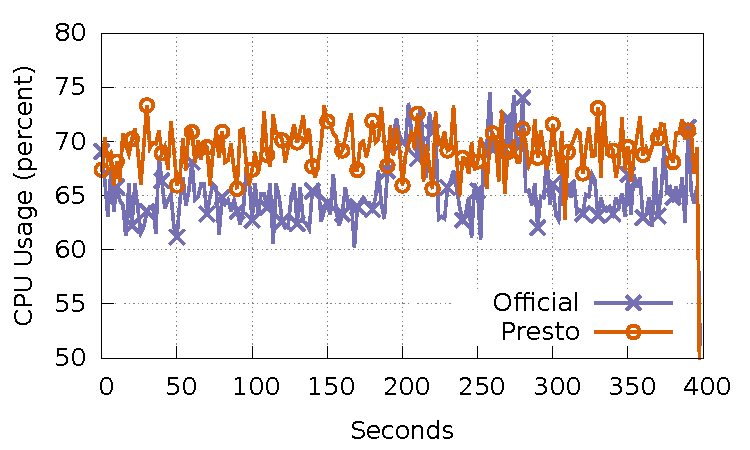
\includegraphics[width=0.45\textwidth]{./figures/mornitor_cpu/macro_compare_cpu_usage.pdf}
        \caption{Presto incurs 6\% CPU overhead on average.}
        \label{micro_compare_cpu}
\end{figure}

\tightparagraph{Presto Imposes Limited CPU Overhead}
We investigate Presto's CPU usage by
running the stride workload on a 2-tier Clos network as shown in Figure~\ref{macro_evaluation_topology}. 
For comparison, official GRO is run with the stride workload using a non-blocking switch (so there
is no reordering). Note both official GRO and Presto GRO can achieve 9.3Gbps.  
The receiver CPU usage is sampled every 2 seconds over a 400 second interval, and
the time-series is shown in Figure~\ref{micro_compare_cpu}. 
%implying that the network utilization is 93% in both cases. 
On average, Presto GRO only increases CPU usage by 6\% compared with the official GRO. 
The minimal CPU overhead comes from Presto's careful design and implementation. 
At the sender, Presto needs just two {\tt memcpy} operations (1 for shadow MAC rewriting, 1 for flowcell ID encoding). 
At the receiver, Presto needs one {\tt memcpy} to rewrite the shadow MAC back to the real MAC and
also incurs slight overhead because multiple segments are now kept per flow. The overhead
of the latter is reduced because these segments are largely kept in reverse sorted order, which means {\tt merge}
on an incoming packet is usually $\mathcal{O}(1)$. The insertion sort is done at the beginning of each {\tt flush} event over a small
number of mostly in-order segments, which easily amortizes overhead because it is called infrequently compared to {\tt merge}.

%%%%%scalability test figures %%%%
\begin{figure}[t]
        \centering
  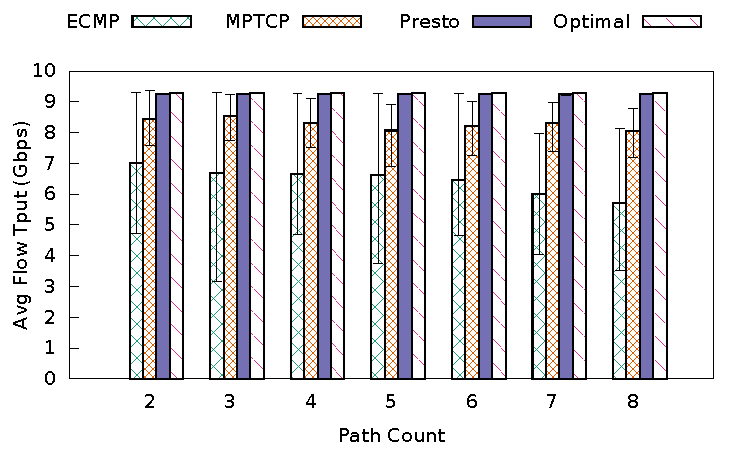
\includegraphics[width=0.45\textwidth]{./figures/scalability_test/scalability_compare_tput_witherrbar.pdf}
        \caption{Throughput comparison in scalability benchmark. We denote the non-blocking case as Optimal. 
		} 
        \label{micro_scalability_test_tput}
\end{figure}

%merged with scalability loss rate
\iffalse
\begin{figure}[ht]
        \centering
  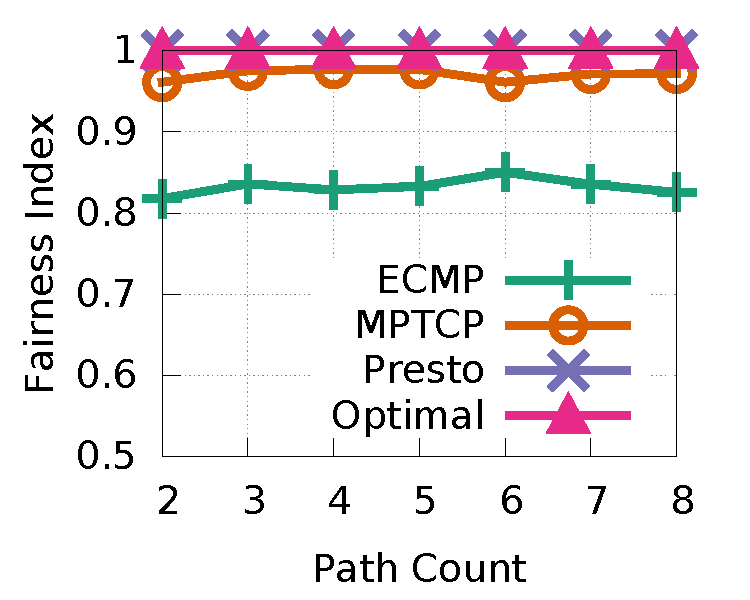
\includegraphics[width=0.45\textwidth]{./figures/scalability_test/scalability_compare_fairness.pdf}
        \caption{Micro benckmark 2 - scalability test. 
		We increase the number of spine switches (i.e., the number of intermediate paths)
                and set the number of flows (host pairs) equal to the number of available paths. 
		Fairness comparison. 20 runs each with each run lasting for 10 seconds.
		Optimal means running TCP on a non-blocking network}
        \label{micro_scalability_test_fairness}
\end{figure}
\fi

\begin{figure}[t]
        \centering
  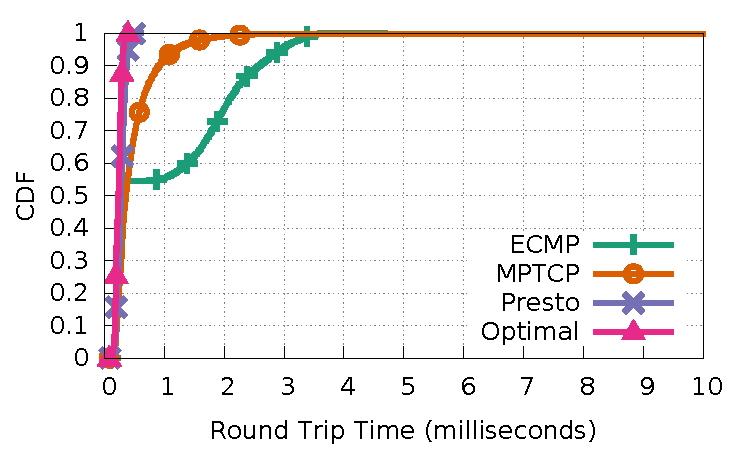
\includegraphics[width=0.45\textwidth]{./figures/scalability_test/scalability_compare_latency.pdf}
        \caption{Round trip time comparison in scalability benchmark. 
		%We increase the number of spine switches (i.e., the number of intermediate paths)
                %and set the number of flows (host pairs) equal to the number of available paths. 
		}
        \label{micro_scalability_test_latency}
\end{figure}


\begin{figure}[t]
        \centering
	\centering
        \begin{subfigure}[b]{0.225\textwidth}
                \centering
		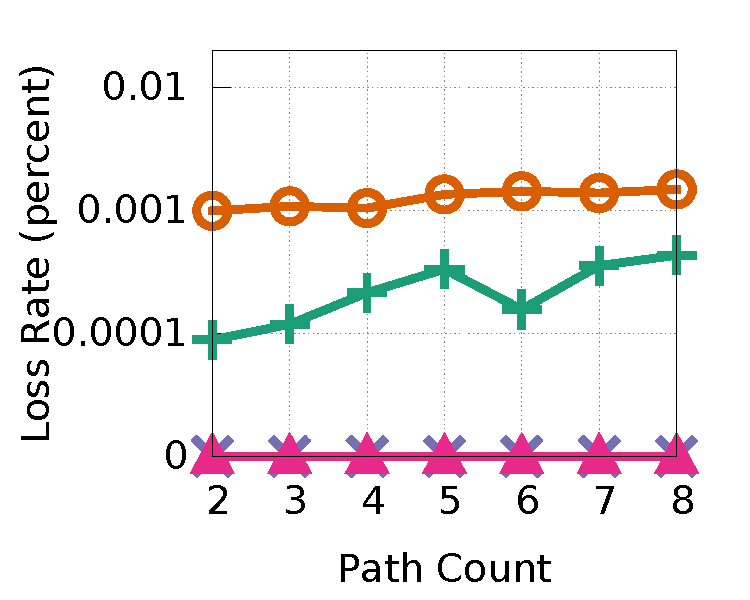
\includegraphics[width=\textwidth]{./figures/scalability_test/scalability_compare_loss.pdf}
		\caption{}
		\label{micro_scalability_test_loss}
        \end{subfigure}
        \begin{subfigure}[b]{0.225\textwidth}
  		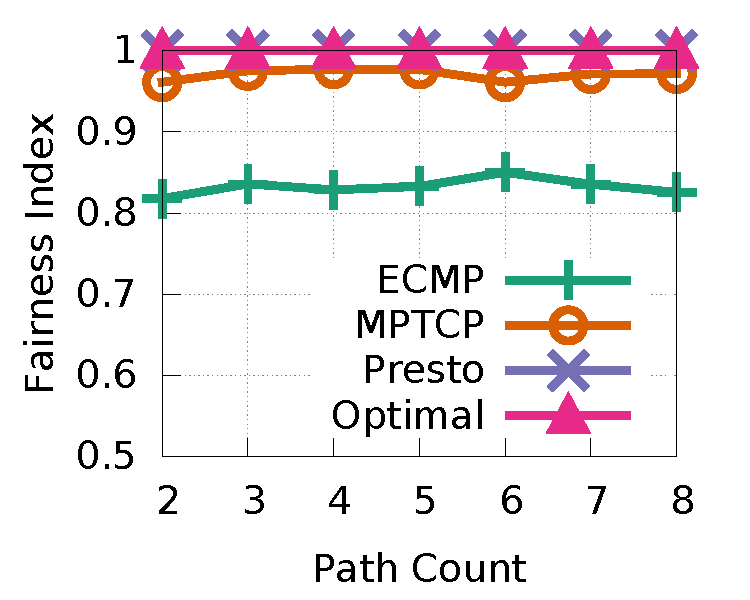
\includegraphics[width=\textwidth]{./figures/scalability_test/scalability_compare_fairness.pdf}
        	\caption{}
        	\label{micro_scalability_test_fairness}
	\end{subfigure}
	\caption{(a) Loss rate and (b) Fairness index comparison in scalability benchmark.}
\end{figure}

\tightparagraph{Presto Scales to Multiple Paths}
We analyze Presto's ability to scale in the number of paths by
setting the number of flows (host pairs) equal to the number of available paths in the topology shown in 
Figure~\ref{micro_scalability_topology}. The number of paths is varied from 2 to 8, and 
Presto always load-balances over all available paths.
Figure~\ref{micro_scalability_test_tput} shows Presto's throughput closely tracks Optimal. 
ECMP (and MPTCP) suffer from lower throughput when flows (or subflows) are
hashed to the same path. Hashing on the same path leads to congestion and thus increased latency, as shown in Figure~\ref{micro_scalability_test_latency}.
Because this topology is non-blocking and Presto load-balances in a near optimal fashion, Presto's latency
is near Optimal. Packet drop rates are presented in Figure~\ref{micro_scalability_test_loss} and show
Presto and Optimal have no loss. MPTCP has higher loss because of its bursty nature~\cite{conga}
and its aggression in the face of loss: when a single loss occurs, only
one subflow reduces its rate. The other schemes are more conservative because a single loss reduces the rate of the whole flow.
Finally, Figure~\ref{micro_scalability_test_fairness} shows Presto, Optimal and MPTCP
achieve almost perfect fairness.
%The underlying reason is that MPTCP makes traffic more bursty~\cite{conga}.


%%%congestion test figures %%%%
\begin{figure}[t]
        \centering
  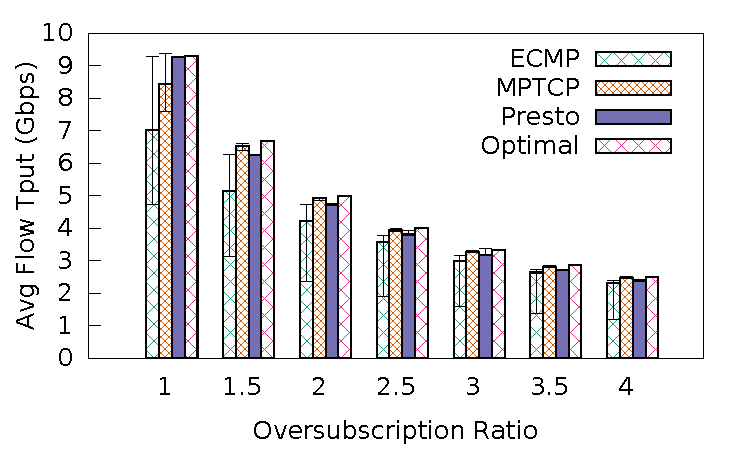
\includegraphics[width=0.45\textwidth]{./figures/congestion_test/congestion_compare_tput_witherrbar.pdf}
        \caption{Throughput comparison in oversubscription benchmark.}
        \label{micro_congestion_test_tput}
\end{figure}


\begin{figure}[t]
        \centering
  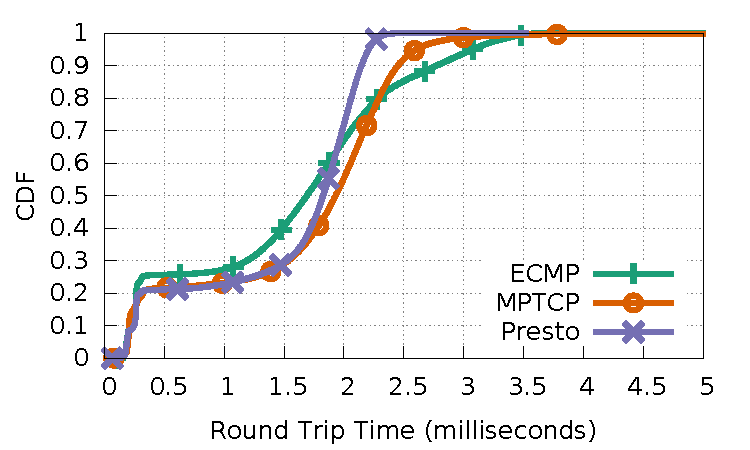
\includegraphics[width=0.45\textwidth]{./figures/congestion_test/congestion_compare_latency.pdf}
        \caption{Round trip time comparison in oversubscription benchmark.
		}
        \label{micro_congestion_test_latency}
\end{figure}



\begin{figure}[t]
        \centering
	\centering
        \begin{subfigure}[b]{0.225\textwidth}
                \centering
		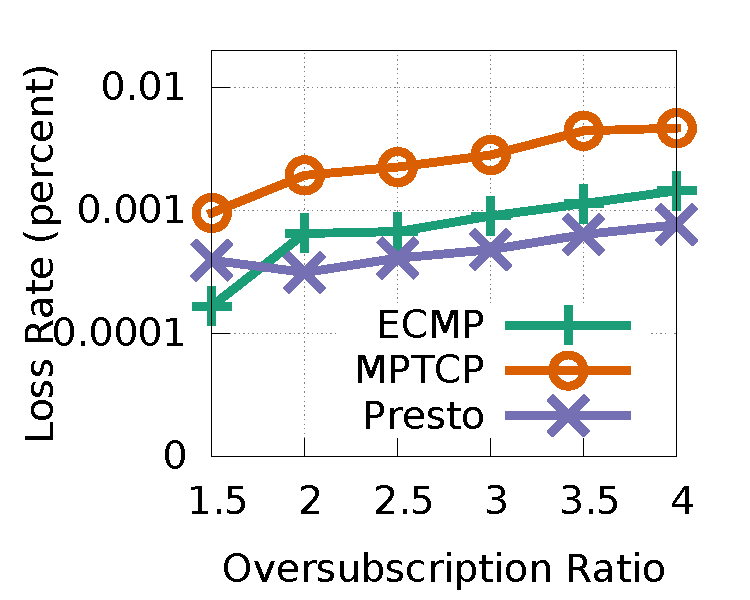
\includegraphics[width=\textwidth]{./figures/congestion_test/congestion_compare_loss.pdf}
		\caption{}
		\label{micro_congestion_test_loss}
	\end{subfigure}
	\begin{subfigure}[b]{0.225\textwidth}
		\centering
  		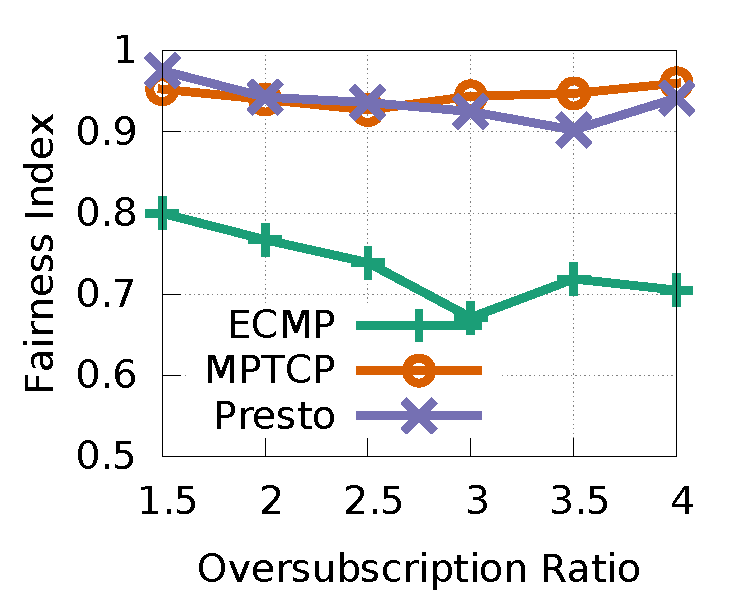
\includegraphics[width=\textwidth]{./figures/congestion_test/congestion_compare_fairness.pdf}
		\caption{}
        \label{micro_congestion_test_fairness}
	\end{subfigure}
	\caption{(a) Loss rate and (b) Fairness index comparison in oversubscription benchmark.}
\end{figure}

\tightparagraph{Presto Handles Congestion Gracefully}
Presto's ability to handle congestion is analyzed by fixing 
the number of spine and leaf switches to 2 and varying
the number of flows (host pairs) from 2 to 8, as shown
in Figure~\ref{micro_congestion_topology}. 
Each flow sends as much as possible, which leads to the network
being oversubscribed by a ratio of 1 (two flows) to 4 (eight flows).
Figure~\ref{micro_congestion_test_tput} shows all schemes track Optimal in highly
oversubscribed environments. ECMP
does poorly under moderate congestion because the limited number of flows can be hashed to the same path.
Presto does no worse in terms of latency (Figure~\ref{micro_congestion_test_latency}) and loss (Figure~\ref{micro_congestion_test_loss}).
The long tail latency for MPTCP is caused by its higher loss rates.
Both Presto and MPTCP have greatly improved fairness compared with ECMP (Figure~\ref{micro_congestion_test_fairness}).

\begin{figure}[t]
        \centering
  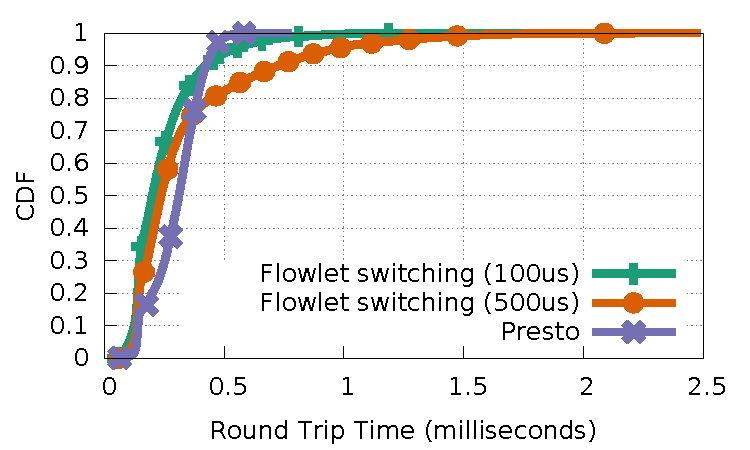
\includegraphics[width=0.45\textwidth]{./figures/flowlets/flowlet_switching/flowlet_presto_compare_sockperf.pdf}
        \caption{Round trip time comparison of Flowlet switching~\cite{flowlet,conga} and Presto in Stride workload. 
		The throughputs of Flowlet switching with 100 $\mu\text{s}$ gap, 500 $\mu\text{s}$ gap and Presto 
		are 4.3Gbps, 7.6Gbps and 9.3Gbps respectively. }
        \label{micro_flowlet_rtt_compare}
\end{figure}


\tightparagraph{Comparison to Flowlet Switching}
We implemented a flowlet load-balancing scheme in OVS that detects
inactivity gaps and then schedules flowlets over disjoint paths in a round robin fashion
(Presto does this over flowcells instead of flowlets).
The receiver for flowlets uses official GRO.
Presto is compared to 500 $\mu$s and 100 $\mu$s inactivity timers in
the stride workload on the 2-tier Clos network (Figure~\ref{macro_evaluation_topology}).
The throughput of the schemes are 9.3 Gbps (Presto), 7.6 Gbps (500 $\mu$s), and 4.3 Gbps (100 $\mu$s).
%Switching flowlets on very small timescales, such as 100$\mu$s, provides opportunities to create many flowlets.
%The largest flowlet is only 0.20\% (XX) of the total network traffic, which corresponds to about 5-9 MB in our runs.
%And while small flowlets create an even distribution
%of traffic over the network, significant strain is put on the TCP connection due to packet reordering. 
Analysis of the 100 $\mu$s
network traces show 13\%-29\% packets in the connection are reordered, which means 100 $\mu$s is not enough
time to allow packets to arrive in-order at the destination and thus throughput is severely impacted. Switching flowlets with 500 $\mu$s prevents
most reordering (only 0.03\%-0.5\% packets are reordered), but creates very large flowlets (see Figure~\ref{micro_flowlet_size}). This means
flowlets can still suffer from collisions, which can hurt throughput (note: while not shown here, 500 $\mu$s outperforms ECMP by over 40\%).
Figure~\ref{micro_flowlet_rtt_compare} shows the
latencies. Flowlet 100 $\mu$s has low throughput and hence lower latencies. However, since
its load balancing isn't perfect, it can still cause increased congestion in the tail. Flowlet 500 $\mu$s
also has larger tail latencies because of more pronounced flowlet collisions. As compared to the flowlet
schemes, Presto decreases 99.9$^{th}$ percentile latency by 2x-3.6x.
%Presto, by enforcing small flowlet sizes and explicitly accounting for reordering on the receiver, can obtain near
%line rate throughput with minimal tail latencies. 



%%%%presto 2 mods (ecmp and shaodw MAC) compare
\begin{figure}[t]
        \centering
  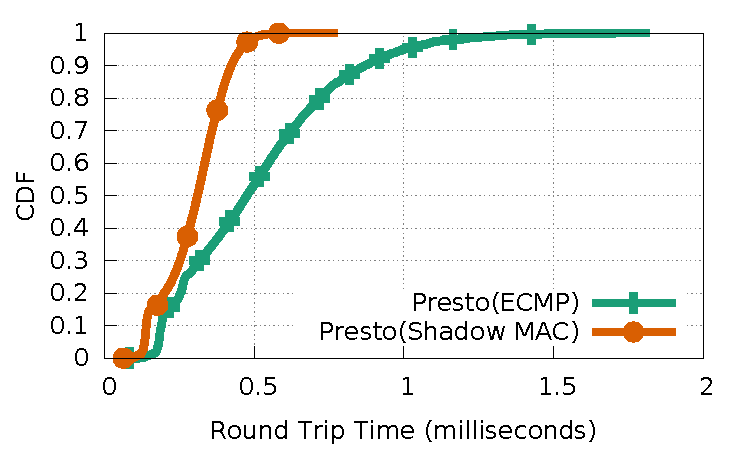
\includegraphics[width=0.45\textwidth]{./figures/presto_compare_2modes/presto_compare_2mods.pdf}
        \caption{Round trip time comparison between Presto + shadow MAC and Presto + ECMP.
		%Compare Presto 2 modes' (Presto over ECMP and Presto over Shadow MAC) performance.
                %Simple 2-tier Clos network with 4 senders and 4 receivers, 4 paths between any host pair.
                %10 seconds per run, 20 runs. Use {\tt nuttcp} to measure throughput. Use {\tt sockperf}
                %to measure latency (RTT).
                %In Presto+ECMP, the average throughput is 7.9 (8.7 if trade latency for tput)
                %Gbps while in Presto+Shadow MAC, the
                %average throughput is 9.3Gbps 
		}
        \label{micro_presto_2mods}
\end{figure}

\tightparagraph{Comparison to Local, Per-Hop Load Balancing}
Presto sends flowcells in a round robin fashion over pre-configured end-to-end paths. An alternative is to
have ECMP hash on flowcell ID and thus provide per-hop load balancing. 
%One way to implement Presto + ECMP is to let vSwitch copy real TCP source port into a pre-allocated TCP option field 
%(\todo{this requires TCP stack allocates the new TCP option before sending to vSwitch}) and 
%encode chunk ID into TCP source port field. Because chunk ID is incremental, ECMP randomly maps chunks into multiple paths. 
We compare Presto + shadow MAC with Presto + ECMP using a stride workload on our testbed. 
Presto + shadow MAC's average throughput is 9.3Gbps while Presto + ECMP's is 8.9Gbps.
The round trip time CDF is shown in Figure~\ref{micro_presto_2mods}. 
Presto + shadow MAC gives better latency performance compared with Presto + ECMP. 
The performance difference comes from the fact that Presto + shadow MAC provides 
better fine-grained flowcell load balancing because 
randomization in per-hop multipathing can lead to corner cases where
a large fraction of flowcells get sent to the same link over a small timescale by multiple flows. This transient congestion
can lead to increased buffer occupancy and higher delays in the network.

\section{Evaluation}
\label{sec:eval}

%~\todo{needs to go through the text and make sure they are consistent with the figures!!!}
In this section, we analyze the performance of Presto for (i) synthetic workloads, (ii)
trace-driven workloads, (iii) workloads containing north-south cross traffic, and (iv) failures.
All tests are run on the topology in Figure~\ref{macro_evaluation_topology}.
\begin{figure}[!t]
        \centering
  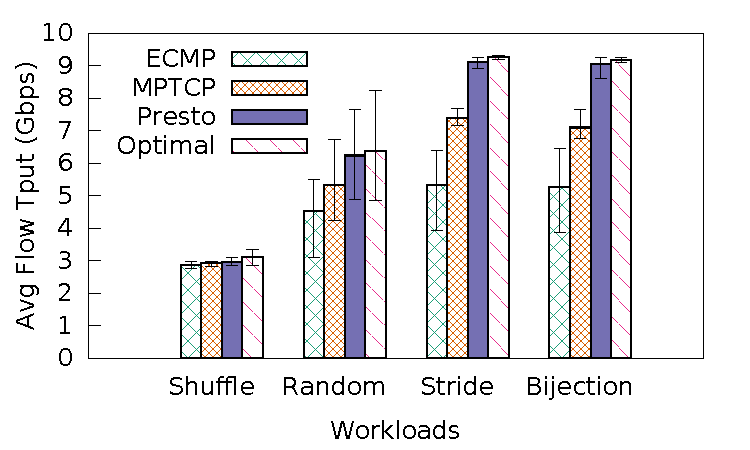
\includegraphics[width=0.5\textwidth]{presto/figures/macro/stride/macro_compare_tput_witherrbar.pdf}
        \caption{Elephant flow throughput for ECMP, MPTCP, Presto and Optimal in shuffle, random, stride and random bijection workloads.}
        \label{macro_evaluation_tput}
\end{figure}



\begin{figure*}[!t]
        \centering
	\begin{subfigure}[b]{0.3\textwidth}
                \centering
  		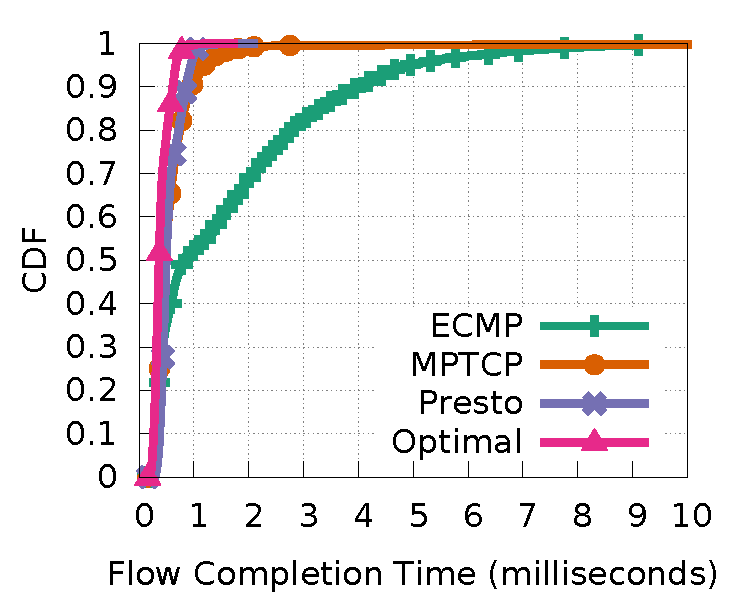
\includegraphics[width=\textwidth]{presto/figures/macro/stride/macro_compare_fct_stride_mice.pdf}
        	\caption{Stride}
        	\label{macro_evaluation_fct_stride}
	\end{subfigure}
	\begin{subfigure}[b]{0.3\textwidth}
                \centering
		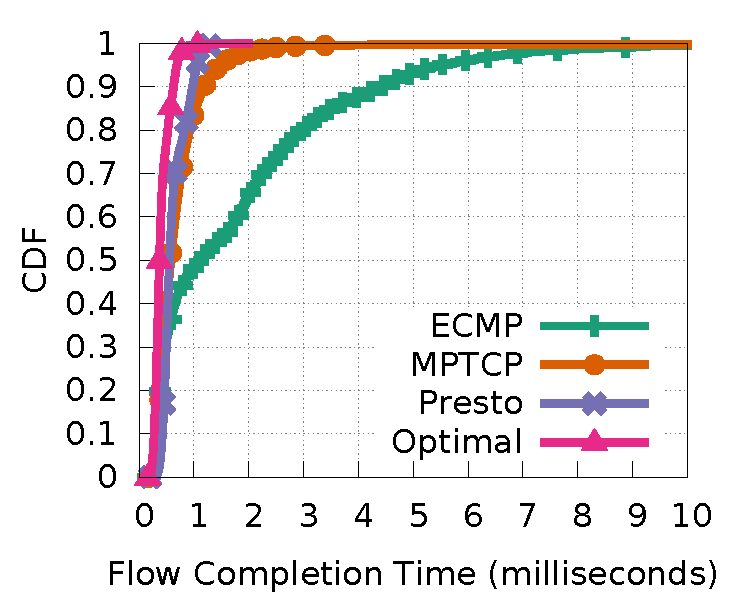
\includegraphics[width=\textwidth]{presto/figures/macro/bijection/macro_compare_fct_bijection_mice.pdf}
        	\caption{Random Bijection}
        	\label{macro_evaluation_fct_bijection}
	\end{subfigure}
        %\begin{subfigure}[b]{0.225\textwidth}
        %        \centering
	%	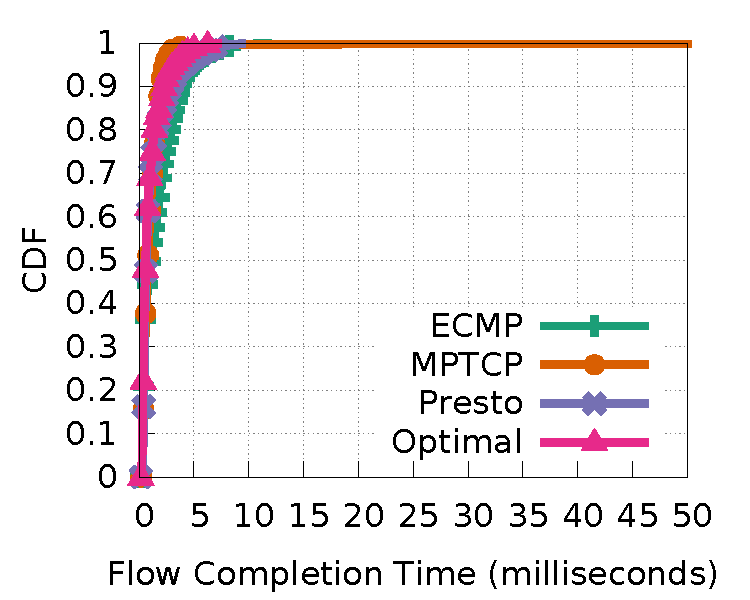
\includegraphics[width=\textwidth]{presto/figures/macro/random/macro_compare_fct_random_mice.pdf}
        %	\caption{Random}
        %	\label{macro_evaluation_fct_random}
	%\end{subfigure}
        \begin{subfigure}[b]{0.3\textwidth}
                \centering
		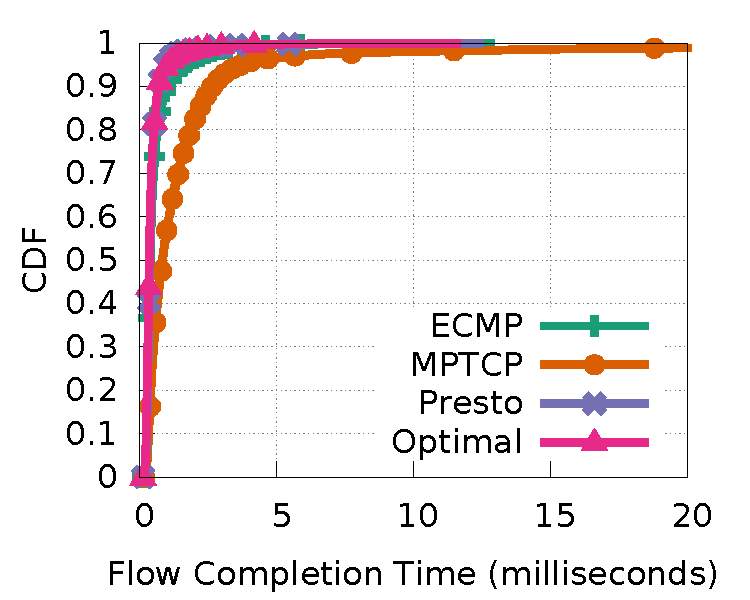
\includegraphics[width=\textwidth]{presto/figures/macro/shuffle/macro_compare_fct_shuffle_mice.pdf}
        	\caption{Shuffle}
        	\label{macro_evaluation_fct_shuffle}
	\end{subfigure}
	\caption{Mice FCT of ECMP, MPTCP, Presto and Optimal in stride, random bijection, and shuffle workloads.}
	\label{macro_evaluation_fct}
\end{figure*}

\tightparagraph{Synthetic Workloads}
Figure~\ref{macro_evaluation_tput} 
shows the average throughputs of elephant flows in the shuffle, random, stride and random bijection workloads.
Presto's throughput is within 1-4\% of Optimal over all workloads.
For the shuffle workload, ECMP, MPTCP, Presto and Optimal show similar results 
because the throughput is mainly bottlenecked at the receiver. 
%due to several servers sending to the same receiver.
In the non-shuffle workloads, Presto improves upon ECMP by 38-72\% and improves
upon MPTCP by 17-28\%.
%Compared with ECMP, 
%Presto improves throughput by 71\% (stride), 72\% (random bijection) and 38\% (random).
%Presto also outperforms MPTCP with throughput improvements of 23\% (stride), 28\% (random bijection) and 
%17\% (random).
%In all the workloads, Presto's throughput outperforms MPTCP.

Figure~\ref{macro_evaluation_fct} shows a CDF of the mice flow completion time (FCT) for each workload.
The stride and random bijection workloads are non-blocking, and hence the latency of Presto
closely tracks Optimal: the 99.9$^{th}$ percentile FCT for Presto is within 350 $\mu$s for these workloads.
MPTCP and ECMP suffer from congestion, and therefore the tail FCT is much worse than Presto: ECMP's 99.9$^{th}$ percentile
FCT is over 7.5x worse ($\sim$11ms) and MPTCP experiences timeout (because of higher loss
rates and the fact that small sub-flow window sizes from small flows can increase the chances of timeout~\cite{dc-mptcp}). We used the Linux default timeout (200 ms) and trimmed graphs for clarity.
The difference in the random and shuffle workloads is less pronounced (we omit random due to space constraints).
In these workloads elephant flows can collide on the last-hop output port,
and therefore mice FCT is mainly determined by queuing latency. In shuffle, the 99.9$^{th}$ percentile FCT for ECMP, Presto and Optimal
are all within 10\% (MPTCP again experiences TCP timeout) and in random, the 99.9$^{th}$ percentile FCT of Presto is within 25\% of Optimal while ECMP's 
is 32\% worse than Presto.


%%the following are combined into one figure
\iffalse
\begin{figure}[!t]
        \centering
  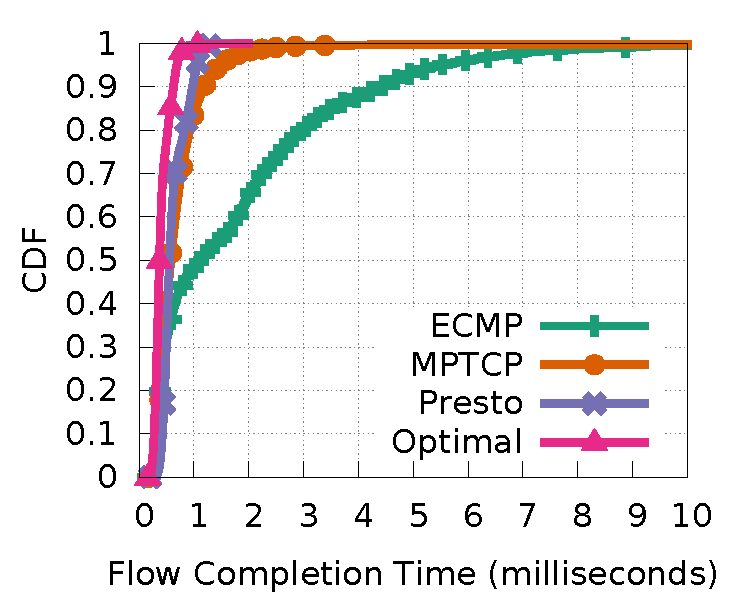
\includegraphics[width=0.45\textwidth]{presto/figures/macro/bijection/macro_compare_fct_bijection_mice.pdf}
        \caption{Macro evaluation - flow completiom time in Random Bijection workload}
        \label{macro_evaluation_fct_bijection}
\end{figure}

\begin{figure}[!t]
        \centering
  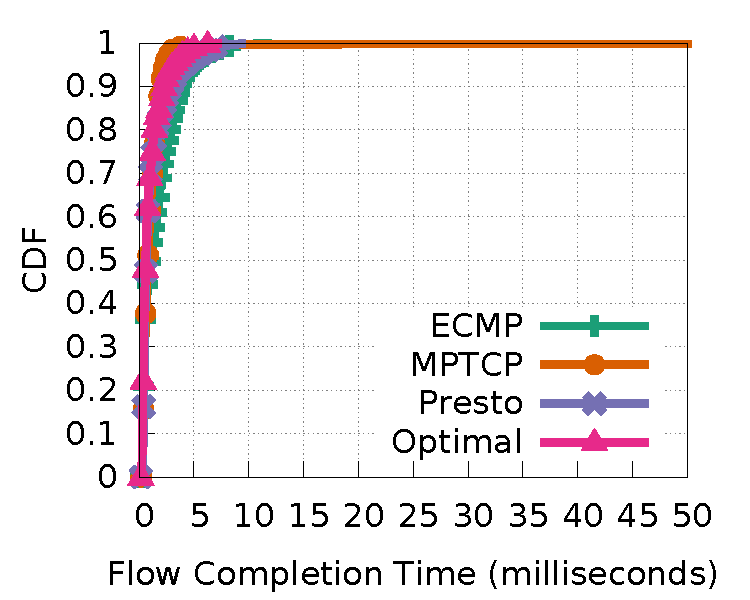
\includegraphics[width=0.45\textwidth]{presto/figures/macro/random/macro_compare_fct_random_mice.pdf}
        \caption{Macro evaluation - flow completiom time in Random workload}
        \label{macro_evaluation_fct_random}
\end{figure}


\begin{figure}[!t]
        \centering
  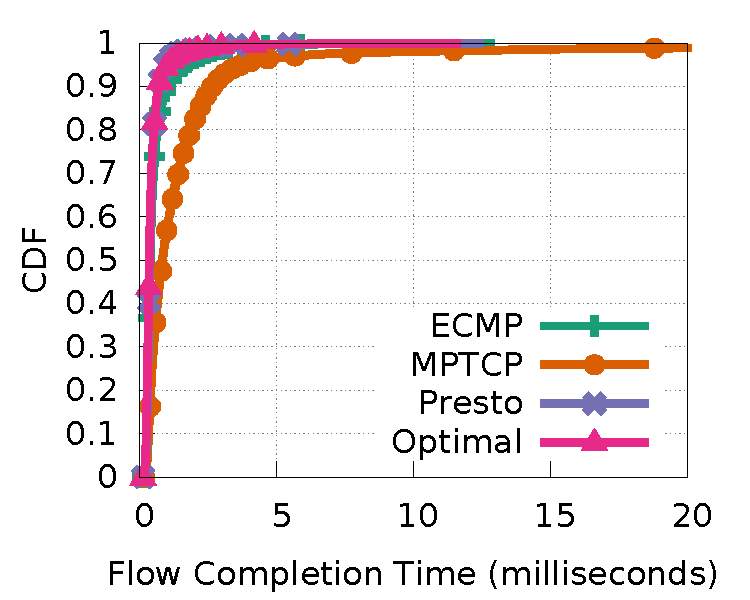
\includegraphics[width=0.45\textwidth]{presto/figures/macro/shuffle/macro_compare_fct_shuffle_mice.pdf}
        \caption{Macro evaluation - flow completiom time in Shuffle workload}
        \label{macro_evaluation_fct_shuffle}
\end{figure}

\fi

\iffalse
\begin{table}[!htb]
\begin{center}
\begin{tabular}{ |c|c|c|c|c| } 
 \hline
 Shuffle & ECMP & MPTCP & Presto & Optimal \\
 \hline 
 Median & 401 & 874 & 387 & 369  \\ 
 90\%   & 1037 & 2664 & 726 & 712 \\
 99\%   & 3373 & 21600  & 2447 & 2446 \\ 
 99.9\% & 12830 & 206ms & 12480 & 11714 \\
 %99.99\% & 204.1ms & - & 204.1ms & 203.6ms \\
 \hline

\end{tabular}
\caption{Macro evaluation - A close look of flow completiom time in Shuffle workload}
        \label{macro_evaluation_fct_shuffle_closelook}
\end{center}
\end{table}

\begin{table}[!htb]
\begin{center}
\begin{tabular}{ |c|c|c|c|c| }
 \hline
 Random & ECMP & MPTCP & Presto & Optimal \\
 \hline
 Median & 1008 & 780 & 648 & 595  \\
 90\%   & 3815 & 1918 & 2850 & 2297 \\
 99\%   & 7852 & 3380  & 6900 & 4936 \\
 99.9\% & 11784 & 202ms & 9372 & 7127 \\
% 99.99\% & 11677 & - & 16591 & 200ms \\
 \hline

\end{tabular}
\caption{Macro evaluation - A close look of flow completiom time in Random workload}
        \label{macro_evaluation_fct_random_closelook}
\end{center}
\end{table}

\fi

%%% trace-driven workload, MSR, scaling factor =10
\begin{table}[!tb]
\begin{center}
\begin{tabular}{ |c|c|c|c| }
 \hline
 Percentile & ECMP & Optimal &Presto \\
 \hline
 50\%   & $1.0$ & $-12\%$ & $-9\%$   \\
 90\%   & $1.0$ & $-34\%$ & $-32\%$  \\
 99\%   & $1.0$ & $-63\%$  & $-56\%$ \\
 99.9\% & $1.0$ & $-61\%$ & $-60\%$  \\
 \hline

\end{tabular}
\caption{Mice ($<$100KB) FCT in trace-driven workload~\cite{kandula2009nature}. Negative numbers imply shorter FCT.}
        \label{macro_evaluation_MSR_trace_driven}
\end{center}
\end{table}

\tightparagraph{Trace-driven Workload}
We evaluate Presto using a trace-driven workload based on traffic patterns measured in~\cite{kandula2009nature}. 
Each server establishes a long-lived TCP connection 
with every other server in the testbed. 
Then each server continuously samples flow sizes and inter-arrival times and each time sends to a random receiver
that is not in the same rack.
%Since 99\% of flows are less than 4MB in the distribution, 
We scale the flow size distribution by a factor of 10 to emulate a heavier workload. 
Mice flows are defined as flows that are less than 100 KB in size, and elephant flows are defined as flows
that are greater than 1 MB. The mice FCT, normalized to ECMP, 
is shown in Table~\ref{macro_evaluation_MSR_trace_driven}. 
Compared with ECMP, Presto has similar performance at the 50$^{th}$ percentile but reduces the 99$^{th}$ and 99.9$^{th}$ percentile FCT by 56\% and 60\%, respectively. 
Note MPTCP is omitted because its performance was quite unstable in workloads
featuring a large number of small flows.
The average elephant throughput (not shown) for Presto tracks Optimal (within 2\%), and improves upon ECMP by over 10\%.


\begin{table}[!htb]
\begin{center}
\begin{tabular}{ |c|c|c|c|c| }
 \hline
% Percentile & 50\% & 90\% & 99\% & 99.9\% \\
% \hline
% ECMP & 1.0 & 1.0 & 1.0 & 1.0  \\
% N-block   & 66\% & 17\% & 11\% & 9\% \\
% Presto    & 80\% & 21\% & 14\% & 10\% \\
% MPTCP     & 88\% & 27\% & 27\% & TIMEOUT \\

 Percentile & ECMP & Optimal & Presto & MPTCP \\
 \hline
 50\%       & 1.0 & $-34$\%     & $-20$\%   & $-12$\% \\
 90\%       & 1.0 & $-83$\%     & $-79$\%   & $-73$\% \\
 99\%       & 1.0 & $-89$\%     & $-86$\%   & $-73$\% \\
 99.9\%     & 1.0 & $-91$\%      & $-87$\%   & TIMEOUT \\

 \hline
\end{tabular}
\caption{FCT comparison (normalized to ECMP) with ECMP load balanced north-south traffic. Optimal means all the hosts are attached to a single  switch.}
	\label{macro_evaluation_north_south_traffic}
\end{center}
\end{table}


\tightparagraph{Impact of North-South Cross Traffic}
Presto load balances on "east-west" traffic in the datacenter, \ie{}, traffic
originating and ending at servers in the datacenter. 
In a real datacenter environment "north-south" traffic (\ie{}, traffic with an endpoint outside the datacenter)
must also be considered. 
%Ideally, north-south traffic should be load balanced by ECMP because of 
%reordering concerns at the end user. 
%However, east-west traffic typically dominates (75\% according to~\cite{east-west}). 
To study the impact of north-south traffic on Presto, we attach an additional server to 
each spine switch in our testbed to emulate remote users. 
The 16 servers establish a long-lived TCP connection with each remote user. 
Next, each server starts a flow to a random remote user every 1 millisecond. This emulates  
the behavior of using ECMP to load balance north-south traffic.
The flow sizes for north-south traffic are based on the distribution measurement in~\cite{he2013next}. 
The throughput to remote users is limited to 100Mbps to emulate the limitation of an Internet WAN. 
Along with the north-south flows, 
a stride workload is started to emulate the east-west traffic. 
The east-west mice FCT is shown in Table~\ref{macro_evaluation_north_south_traffic} (normalized to ECMP). 
ECMP, MPTCP, Presto, and Optimal's average throughput is 
5.7, 7.4, 8.2, and 8.9Gbps respectively. 
The experiment shows Presto can gracefully co-exist with north-south cross traffic
in the datacenter.


%%%failure handling experiments

\begin{figure}[!t]
        \centering
  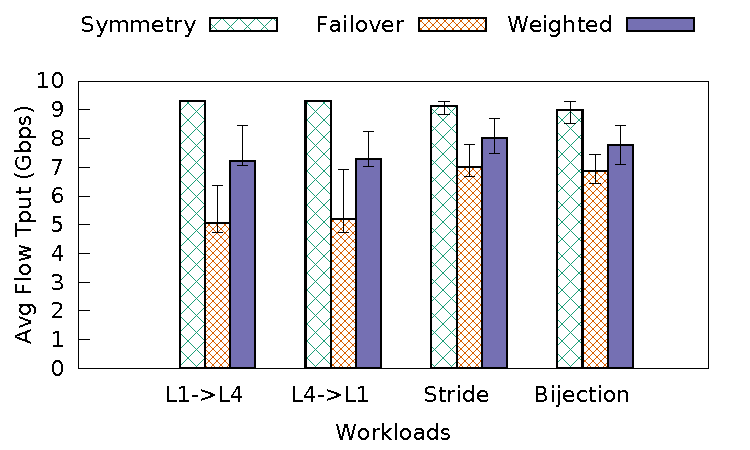
\includegraphics[width=0.5\textwidth]{presto/figures/failure_handling/failover_compare_tput_witherrbar.pdf}
        \caption{Presto's throughput in symmetry, fast failover and weighted multipathing stages for different workloads.}
        \label{failover_compare_tput}
\end{figure}

\begin{figure}[!t]
        \centering
  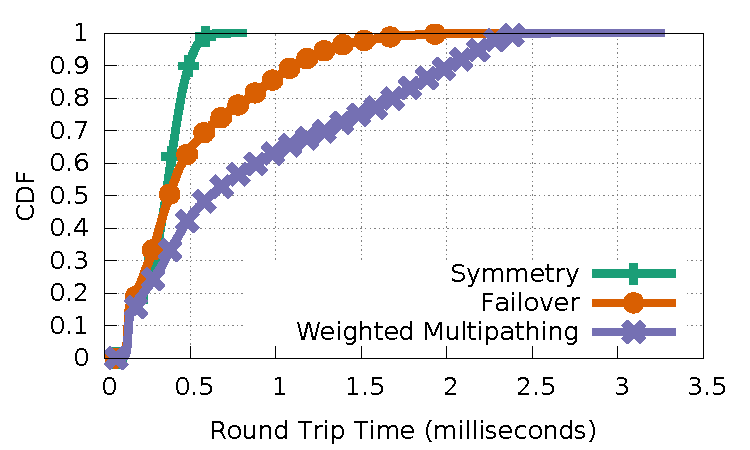
\includegraphics[width=0.5\textwidth]{presto/figures/failure_handling/failover_compare_sockperf_bijection_mice.pdf}
        \caption{Presto's RTT in symmetry, fast failover and weighted multipathing stages in  random bijection workload.}
        \label{failover_compare_sockperf_bijection}
\end{figure}

\tightparagraph{Impact of Link Failure}
Finally, we study the impact of link failure.
Figure~\ref{failover_compare_tput} compares the throughputs of
Presto when %under different stages of loss recovery when 
the link between spine switch S1 and leaf switch L1 goes down.
Three stages are defined: symmetry (the link is up), failover (hardware fast-failover moves traffic from S1 to S2), and weighted (the controller
learns of the failure and prunes the tree with the bad link).
Workload L1$\rightarrow$L4 is when each node connected to L1 sends to one node in L4 (L4$\rightarrow$L1 is the opposite).
Despite the asymmetry in the topology, Presto still achieves reasonable average throughput at 
each stage.
Figure~\ref{failover_compare_sockperf_bijection} shows the round trip time of
each stage in a random bijection workload. 
Due to the fact that the network is no longer non-blocking after the link failure,
failover and weighted multipathing stages have larger round trip time.



\iffalse
\begin{enumerate}
\item Clos-network, macro. ECMP, MPTCP, Presto and Optimal.
\begin{enumerate}
	\item Workloads: Take from Planck and Hedera. Can do MSR trace-based.
	\item Throughput, fairness, latency (maybe loss). Link utilization?
\end{enumerate}

\item Fat tree, macro. ECMP, MPTCP, Presto and Optimal.
\begin{enumerate}
        \item Workloads: Take from Planck and Hedera. Can do MSR trace-based.
        \item Throughput, fairness, latency (maybe loss). Link utilization?
\end{enumerate}


\item Vary flow sizes. Idea is that we can work on very small elephants.

\item Failure: backbone switch fails, aggregate switch fails, ToR switch fails, link fails, ...

\item CONGA uses incast, should we check?

\item Maybe this belongs in micro: ECMP vs shadowMAC for multipathing.

\end{enumerate}
\fi

%\section{Related Work}
\label{sec:related}
We summarize the related work into three categories: datacenter traffic load balancing, reducing tail latency and handling packet reordering.

{\bf Load Balancing in Datacenters} 
%Load balancing in datacenter networks has been the focus of several studies.
MPTCP~\cite{mptcp,dc-mptcp} is a transport protocol that uses subflows to 
transmit over multiple paths.
CONGA~\cite{conga} and Juniper VCF~\cite{juniper-vcf} both employ congestion-aware flowlet switching~\cite{flowlet} on
specialized switch chipsets to load balance the network.
RPS~\cite{packetspray} and DRB~\cite{drb} evaluate per-packet load balancing on symmetric 1 Gbps networks
at the switch and end-host, respectively.
The CPU load and feasibility of end-host-based per-packet load balancing for 10+ Gbps networks remains open.
%Per-packet load balancing can incur significant end-host overhead for DRB
%if not resorting to jumbo frames.
%Packet reordering problem is not well considered in both RPS and DRB.
%RPS and DRB may perform worse than ECMP in case of topology asymmetry.
Hedera~\cite{hedera}, MicroTE~\cite{microte} and Planck~\cite{planck} use centralized traffic engineering to
reroute traffic based on network conditions.
FlowBender~\cite{flowbender} reroutes flows when congestion is detected by end-hosts and 
Fastpass~\cite{fastpass} employs a centralized arbiter to schedule path selection for each packet.
As compared to these schemes, Presto is the only one that proactively load-balances at line rate for fast networks
in a near uniform fashion without requiring additional infrastructure or changes
to network hardware or transport layers. Furthermore, to the best of our knowledge, Presto is
the first work to explore the interactions of fine-grained load balancing with built-in
segment offload capabilities used in fast networks.
%\textcolor{blue}{~\cite{eden} also advocates to implement network functions such as load balancing 
%at datacenter end hosts.}

{\bf Reducing Tail Latency}
%Detail~\cite{detail} summarizes the causes of long tails of flow completion time---
%1)packet loss and retransmissions,
%2)absence of flow prioritization and 3)uneven load balancing.
%Reducing tail latencies of small mice flows has also been actively studied.
DeTail~\cite{detail} is a cross-layer network stack designed to reduce the tail of flow completion times.
%link layer uses port buffer occupancy to construct lossless fabric,
%network layer performs per-packet adaptive load balancing based on port buffer occupancy,
%transport layer relies upon congestion notifications
%derived from port buffer occupancies,
%finally Detail lets application layer specify flow priorities to
%avoid head-of-line blocking of elephant flows for mice time-sensitive flows.
%Detail modified many layers (including the switch) and is hard to deploy using
%current hardware and network stack.
DCTCP~\cite{dctcp} is a transport protocol that uses the portion of marked packets 
by ECN to adaptively adjust sender's TCP's congestion window to reduce switch buffer occupancy.
%Thus, DCTCP can reduce switch buffer occupancy and reduce flow completion time.
HULL~\cite{hull} uses Phantom Queues and congestion notifications to cap link utilization and prevent congestion.
%HULL uses packet pacing to combat with traffic burstiness in order to leave "bandwidth headroom".
In contrast, Presto is a load balancing system that naturally improves 
the tail latencies of mice flows by uniformly spreading traffic in 
fine-grained units.
%We share the overall goal of reducing mice tail latencies, but instead explore how
%fine-grained load balancing can provide a solution.
QJUMP~\cite{qjump} utilizes priority levels to 
allow latency-sensitive flows to "jump-the-queue" over low priority flows.
PIAS~\cite{pias} uses priority queues to mimic the Shortest Job First principle to reduce FCTs.
%solve the network interference problem caused by elephant and mice flows 
%for datacenter networks. High priority packets are rate-limited 
%at the end-host and can "jump-the-queue" over packets with 
%lower priorities. PIAS~\cite{pias} mimics the Shortest Job First (SJF) 
%principle to reduce flow completion times. It gradually decreases 
%the priority level assigned to a flow based on its flow size.
%Presto is complementary and could be applied on each priority level.
%DIBS~\cite{dibs} detours packets of a congested switch port to a randomly 
%picking neighboring switch to reduce packet drops.
Last, a blog post by Casado and Pettit~\cite{vmware} summarized
four potential ways to deal with elephants and mice, with one advocating
to turn elephants into mice at the edge. 
We share the same motivation and high-level
idea and design
a complete system that addresses many practical challenges of using
such an approach.

%%%%%the follwoing may not be used
\iffalse
WCMP~\cite{wcmp} reduces the number of TCAM/SRAM entries to implement 
Weighted Cost Multipathing for asymmetry network topologies 
by approximating the path weights. 
Different from WCMP, Presto assigns path weights in openvswitch (i.e., host memory), 
thus Presto is not limited by TCAM resource. 
Similar to WCMP, Presto can perform near-optimal traffic striping in asymmetry topologies because
the weights are determined by a global view of the network.

VL2~\cite{vl2} uses flat addressing to allow service instances to be placed anywhere in the network. 
It leverages a shim-layer on end-hosts to perform IP-in-IP encapsulation to 
decouple topological address from flat application address.
Portland~\cite{portland} uses positional pseudo MAC address to decouple forwarding address from service address. 
VXLAN~\cite{vxlan} and NVGRE~\cite{nvgre} use tunneling mechanism (virtualized L2 networks over L3 network) to 
enable applications to be deployed and migrated between any server regardless of physical server location. 
Presto achieves Ethernet L2 semantics via employing shadow MAC~\cite{shadow-mac}, 
where shadow MAC serves as forwarding address while providing the opportunity to do load balancing.
\fi

{\bf Handling Packet Reordering}
%Many schemes have tried to mitigate the impact of reordering.
TCP performs poorly in the face of reordering, and thus several studies
design a more robust alternative~\cite{rr-tcp,blanton2002making,tcp-pr}.
Presto takes the position that reordering should be handled below TCP in the existing 
receive offload logic.
In the lower portion of the networking stack, SRPIC~\cite{wu2009sorting} sorts reordered packets 
in the driver after each interrupt coalescing event. While this approach can help
mitigate the impact of reordering, it does not sort packets across interrupts, have a 
direct impact on segment sizes, or distinguish between loss and reordering. 
%SRPIC is 
%complementary to our approach because their actions are taken in the driver, before packets
%are pushed to GRO.
%RR-TCP~\cite{rr-tcp} proposed to extend TCP sender to detect and recover from false fast retransmits using DSACK information. 
%As we show, fixing TCP itself cannot solve all the problems incurred by packet reordering.
%\eric{i have some LRO references in the patent slides that we need to make sure are cited somewhere} 
%Instead, Presto's chunking scheme leverages the fact that all the packets going through the same path are in order and has two nice properties:
%1)Presto uses chunkid to make the task of distinguishing packet loss from temporary packet reordering much simpler. 
%2)Presto only needs to make sure the chunks are in order instead of packets, thus reducing per-packet processing overhead.

%\section{Discussion}
\label{discuss}

\tightparagraph{UDP traffic} How to handle. 
Mention VxLAN traffic too.
\keqiang{and IPsec}

\tightparagraph{No vSwitch} 
\keqiang{title should be hypervisor-bypass?}
Use middleboxes (for DB server).
Use NIC (for SR-IOV).
Hypervisor bypass (e.g., SR-IOV), where TCP traffic is sent to the NIC directly without 
going through hypervisor. First, as noted by~\cite{shieh2011sharing}, ``loss of the security and 
manageability features provided by the software virtual switch has limited 
the deployment of direct I/O NICs in public clouds''. Second, based on techniques like Intel 
DPDK~\cite{intel-dpdk} and ``smart NICs''~\cite{cavium-nic,netronome-nic}, we believe that low latency 
congestion control enforcement schemes like \acdc{} can also be 
employed for hypervisor bypass use cases.
We need to worry about legacy systems and non-VM systems. For instance, a database or storage device that may not have OVS installed on it.
We need to talk about either a middlebox or that this percentage of traffic is low? Or implement in NIC (especially one with OVS offload?).

\tightparagraph{North-South traffic.}
Transport enforcement should be only be done for east west traffic, so if the tenant tuned their stack's
congestion control algorithm for wide-area networks, their north sourth traffic is not affected and their 
congestion control scheme can still achieve good performance.

\keqiang{todos: some figures do not read well on printed paper}
\keqiang{todos: sometimes, when we refer a section, we say ``Section X'', sometimes, we use the 
dollar sign, we should unify them}

%
%Byzantine VM.
%
%Other names: ACDCTCP, LiquidSwitch, LiquidEdge
%
%In CPU overhead measurement, we need to 
%mention ovs add 1 widecard rule. That means we isolated the overhead of 
%OVS itself when it has many flows in its flow table (probably it does not matter
%at the end of the day, because we measured the CPU usage of the whole system).
%
%People may say window-based congestion control is burty. TIMELY operates 
%on TCP segments in order to reduce CPU overhead. Therefore, TIMELY is also
%busty. In TIMELY, they mentioned they can leverage a hybrid scheme, that is
%using software to control large segments and use hardware rate limiter to
%reduce burstyness.
%
%Create loss and check how DCTCP and our scheme treates packet losses (revisit it after we finish incast 
%and macrobenchmarks).
%
%One more microbenchmark on the Dumbbell topology: different servers have different transport, so the
%throughput fairness among different transports (e.g., start cubic, start New Reno, start dctcp).
%
%A point that is missing in DCTCP and NSDI paper is that they did not mention how the switch should be
%configured to handle non-TCP traffic. Note non-TCP traffic such as DNS (UDP 53) and ARP, ICMP etc
%are also important. We found that if we did not specify how the switch handle the non-TCP traffic,
%then this kind of non-TCP traffic can be easily dropped by the switch. We found ARP traffic is dropped
%by the switch such that DCTCP flows stall. Hence, we think it is better to put non-TCP traffic
%into a different queue when we apply WRED/ECN on the switches.
%
%This work offers low latency for ``hetergeneous networks" where different entities can 
%run different kinds of
%transport congestion control schemes. A few examples of such hetergeneous networks: public 
%datacenters where tenants can set up their own VMs (e.g., AWS), or tenants can rent their bare metal
%machines (e.g., SoftLayer), or certain groups (even within a single organization) 
%have to use traditional transports due to compatibility of legacy applications (NSDI's Judd said this), or
%incremental deployment is undergoing. 
%To ensure a pure low latency datacenter network, a universal transport enforcement scheme is required. 
%Two challenges to implement such a transport enforcement scheme are scalability and low overhead. 
%The transport enformancement scheme proposed here meet the two metrics (as shown in our experiments) while
%providing nice network performance (throughput, latency and packet drop rate). This scheme is 
%compatible with any kind of TCP stack. Finally, the scheme we propose solves the co-existence issue of 
%ECT (ECN Capable Transport) and non-ECT, which is a critical deployment hurdle for DCTCP-like transports.
%
%Macrobenchmark plan: 18 hosts, 6 switches, ECMP configured. The network oversubscription ratio is 2:1.
%Run all-to-all traffic for a long time (e.g., 1 hours). Show total throughput and TCP RTT and packet drop 
%rate.
%
%QoS can be implemented too?
%
%
%
%When we try to launch an instance in EC2: ``An AMI is a template that contains the software 
%configuration (operating system, application server, and applications) required to launch your instance. 
%You can select an AMI provided by AWS, our user community, or the AWS Marketplace; 
%or you can select one of your own AMIs''. Default is CUBIC for most Linux images, Window Servers can
%have NewReno, Compound TCP (CTCP)~\cite{tan2006compound} and DCTCP. 
%Users can tweak congestion control algorithms to optimize network performance for their target scenarios. 
%
%Section talking about how to implement other CC schemes: TIMELY, PERC, Vegas, etc.
%
%EJR: VXLAN, UDP, TCP stack statistics for Cloud?
%
%ECT and non-ECT: througput unfairness, long RTT, connection establishment..
%
%
%EyeQ, Seawall, NetShare, Silo, SecondNet, Oktopus etc. Our work did not provide bandwidth allocation property. 
%This work focused on reducing in-network queuing latency caused by VM TCP stacks. 
%We show how this goal can be done using a simple and elegant solution.
%Yes, if an VM opens more connections than another, that VM gains more bandwidth. 
%But, there are proposals which try to provide proper bandwidth allocation when multiple end-points compete 
%at the sender side or receiver side. Those works and this work are complementary. 
%To the best of our knowledge, today's cloud providers have not provide strong bandwidth guarantees 
%(for example, AWS only roughly classify VMs instances' network performance into 
%``low to moderate", ``moderate", ``high" and ``10 Gigabit"categories).
%
%talk about containers?

\section{Summary}
\label{sec:conclusion}
In this chapter, we present Presto: a near uniform sub-flow distributed load balancing scheme
that can near optimally load balance the network at fast networking speeds.
Our scheme makes a few changes to the hypervisor soft-edge (vSwitch and GRO)
and does not require any modifications to the transport layer or network hardware, making
the bar for deployment lower. 
%Working at fast networking speeds poses many challenges,
Presto is explicitly designed to load balance the network at fine granularities
and deal with reordering without imposing much overhead on hosts. Presto is flexible and can also
deal with failures and asymmetry. Finally, we show the performance of Presto can closely track
that of an optimal non-blocking switch, meaning elephant throughputs remain high while the tail
latencies of mice flow completion times do not grow due to congestion.



\chapter{Virtual Congestion Control Enforcement for Datacenter Networks}

\section{Introduction}
\label{intro}

Multi-tenant datacenters are a crucial component of today's computing ecosystem. Large providers, such as Amazon, Microsoft, IBM, Google and Rackspace, support
a diverse set of customers, applications and systems through their public cloud offerings. These offerings are successful in 
part because they provide efficient performance to a wide-class of applications running on a diverse set of platforms. Virtual
Machines (VMs) play a key role in supporting this diversity by allowing customers to run applications in a wide variety of 
operating systems and configurations.

And while the flexibility of VMs allows customers to easily move a vast array of applications into the cloud, that same flexibility inhibits the 
amount of control a cloud provider yields over VM behavior. For example, a cloud provider may be able to provide virtual networks or enforce rate limiting
on a tenant VM, but it cannot control the VM's TCP/IP stack. As the TCP/IP stack considerably impacts overall network performance, it 
is unfortunate that cloud providers cannot exert a fine-grained level of control over one of the most important components in the networking stack.

Without control over the VM TCP/IP stack, datacenter networks remain at the mercy of inefficient, out-dated or misconfigured TCP/IP stacks.
TCP behavior, specifically congestion control, has been widely studied and many issues have come to light when it is not optimized. For example,
network congestion caused by non-optimzed stacks can lead to loss, increased latency and reduced throughput. 
%As revenue increasingly is tied to 
%strict latency and bandwidth requirements from workloads such as big data analytics and search~\cite{alizadeh2011data,dean2013tail}, public cloud providers must ensure their
%network fabrics can provide tight service-level agreements and deadlines required by customer applications.

Thankfully, recent advances optimizing TCP stacks for datacenters have shown high throughput and low latency can be 
achieved through novel TCP congestion control algorithms. Works such as DCTCP~\cite{alizadeh2011data} and TIMELY~\cite{mittal2015timely} provide high
bandwidth and low latency by ensuring network queues in switches do not fill up. And while these stacks are deployed in many of today's 
private datacenters~\cite{singh2015jupiter,judd2015nsdi}, ensuring a vast majority of VMs within a public datacenter will update their TCP stacks
to a new technology is a daunting, if not impossible, task.

In this chapter, we explore how operators can regain authority over TCP congestion control, regardless of the TCP stack
running in a VM. Our aim is to allow a cloud provider to utilize advanced TCP stacks, such as DCTCP, without having
control over the VM or requiring changes in network hardware. We propose implementing congestion control in the virtual switch
(vSwitch) running on each server. Implementing congestion control within a vSwitch has several advantages. 
First, vSwitches naturally fit into datacenter network virtualization architectures and are widely
deployed~\cite{Pfaff2015ovs}. Second, vSwitches can easily monitor and modify traffic passing through them. 
Today vSwitch technology is mature and robust, allowing for a fast, scalable,
and highly-available framework for regaining control over the network. 

%Since vSwitch technology supports software-defined networking (say OVS),
%implementing congestion control within the vSwitch can also naturally support advanced congestion control algorithms, such as centralized 
%or proactive schemes (cite). 

Implementing congestion control within the vSwitch has numerous challenges, however. First, in order to ensure adoption rates are high, the 
approach must work without making changes to VMs. 
Hypervisor-based approaches typically rely on rate limiters to limit VM traffic. Rate limiters implemented in
commodity hardware do not scale in the number of flows and software implementations incur high CPU overhead~\cite{radhakrishnan2014senic}. 
Therefore, limiting a VM's TCP flows in a fine-grained, dynamic nature
at scale (10,000's of flows per server~\cite{180302}) with limited computational overhead remains challenging. 
Finally, VM TCP stacks may differ in the features they support (\eg{}, ECN) or the congestion
control algorithm they implement, so a vSwitch congestion control implementation should work under a variety
of conditions. 

This chapter presents Administrator Control over Datacenter TCP (\acdc{} TCP, or simply~\acdc{}), a new technology that implements 
TCP congestion control within a vSwitch to help ensure VM
TCP performance cannot impact the network in an adverse way. At a high-level, the vSwitch monitors all packets for a flow, modifies 
packets to support features not implemented in the VM's TCP stack (\eg{}, ECN) and reconstructs
important TCP parameters for congestion control.~\acdc runs the congestion control logic specified by an administrator and then enforces an intended
congestion window by modifying the receive window (\rwnd{}) on incoming ACKs. A policing
mechanism ensures stacks cannot benefit from ignoring~\rwnd{}.% and can also be used for non-TCP traffic.

Our scheme provides the following benefits. First,~\acdc allows
administrators to enforce a uniform, network-wide congestion control algorithm without changing VMs. When using congestion control algorithms tuned for 
datacenters, this allows for high throughput and low latency. Second,
our system mitigates the impact of varying TCP stacks running on the same fabric. This improves fairness and additionally
solves the ECN co-existence problem identified in production networks~\cite{wu2012tuning,judd2015nsdi}. 
Third, our scheme is easy to implement, computationally lightweight, scalable, and modular so that it is highly complimentary to
performance isolation schemes also designed for virtualized datacenter environments.
The contributions of this chapter are as follows:
\begin{enumerate}
\item The design of a vSwitch-based congestion control mechanism that regains control over the VM's TCP/IP stack
without requiring any changes to the VM or network hardware. 
\item A prototype implementation to show our scheme is effective, scalable, simple to implement, and has~\crs{less than one percentage point} computational overhead in our tests.
%~\todo{We also provide a simple policing scheme to see if tenants are following rules. Add?} 
\item A set of results showing DCTCP configured as the host TCP stack provides nearly identical
performance to when the host TCP stack varies but DCTCP's congestion control is implemented in the vSwitch. We demonstrate how~\acdc{} can improve
throughput, fairness and latency on a shared datacenter fabric.
\end{enumerate}

The outline of this chapter is as follows. Background and motivation are discussed in \cref{background}.~\acdc{}'s design is outlined in \cref{design} and
implementation in \cref{impl}. Results are presented in \cref{results}.


\section{Background and Motivation}
\label{background}
This section first gives a brief background of congestion 
control in the datacenter. Then the motivation for moving congestion
control into the vSwitch is presented. Finally,~\acdc{} is contrasted from a class of related bandwidth
allocation schemes.

\subsection{Datacenter Transport}
\label{ss:dct}
Today's datacenters host applications such as search,
advertising, analytics and retail that require high bandwidth and low latency.
%Large tail latencies often violate the tight timing constraints required by SLAs at scale, and
%have been shown to impact customer experience, result in
%revenue loss~\cite{alizadeh2011data,dean2013tail}, and degrade application performance~\cite{jang2015silo,qjump}.
%Tail latencies are often caused by network congestion.
%The latency of traversing a single switch, NIC and OS network stack is 10--30$\mu$s,
%2.5--32$\mu$s and 15$\mu$s respectively, but a congested port
%on a network switch can consume significant shared memory, causing orders-of-magnitude
%higer latency~\cite{rumble2011s}.
Network congestion, caused by imperfect load balancing~\cite{al2010hedera},
network upgrades or failures, can adversely impact these services. Unfortunately, congestion is
not rare in datacenters. For example, recently Google reported 
congestion-based drops were observed when network utilization approached 25\%~\cite{singh2015jupiter}.
Other studies have shown high variance and substantial increase in the 99.9$^{th}$ percentile latency
for round-trip times in today's datacenters~\cite{wang2010impact,mogul2015inferring}. 
Large tail latencies impact customer experience, result in
revenue loss~\cite{alizadeh2011data,dean2013tail}, and degrade application performance~\cite{jang2015silo,qjump}.
Therefore, significant motivation exists to reduce congestion in datacenter fabrics.

%Studies have shown that while CUBIC can achieve
%high bandwidth, it does so at the cost of aggressively filling up the switch buffers in the network.
TCP's congestion control algorithm is
known to significantly impact network performance.
As a result, datacenter TCP performance has been widely
studied and many new protocols have been proposed~\cite{alizadeh2011data, stephens2014practical, wu2010ictcp,
mittal2015timely, jose2015high}. Specifically, DCTCP~\cite{alizadeh2011data} adjusts a TCP sender's rate based on the fraction of packets experiencing congestion. In DCTCP,
the switches are configured to mark packets with an ECN bit when their queue lengths exceed a threshold. By proportionally
adjusting the rate of the sender based on the fraction of ECN bits received, DCTCP can keep queue lengths low, 
maintain high throughput, and increase fairness and stability over traditional schemes~\cite{alizadeh2011data,judd2015nsdi}.
\crs{For these reasons, we implement DCTCP as the vSwitch congestion control algorithm in~\acdc{}.}

\subsection{Benefits of~\acdc{}}
%Rather than proposing a new datacenter congestion control algorithm, this work investigates
%if congestion control can be moved to the vSwitch.
Allowing administrators to enforce an optimized congestion control without
changing the VM is the first major benefit of our scheme.
This is an important criteria in untrusted public cloud environments or simply in cases where servers cannot be updated
due to a dependence on a specific OS or library.~\cite{judd2015nsdi}


\begin{figure}[!t]
        \centering
        \begin{subfigure}[b]{0.225\textwidth}
                \centering
		%max min mean median
                %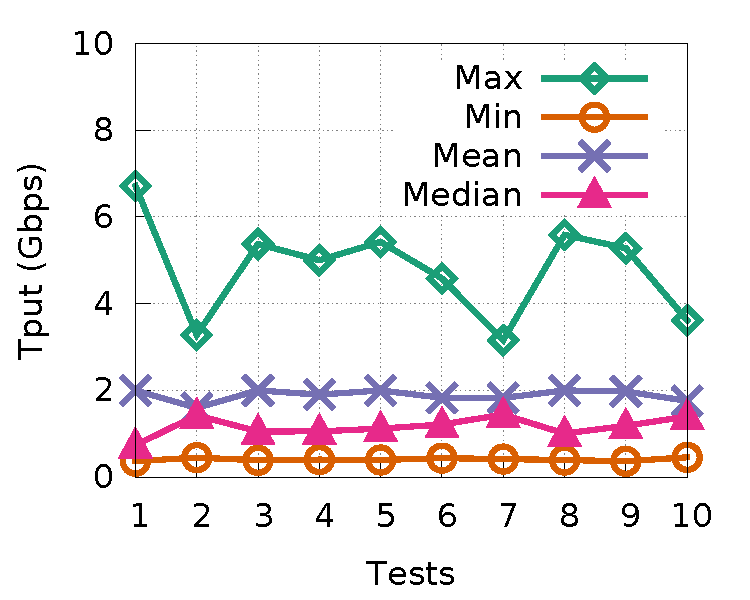
\includegraphics[width=\textwidth]{acdctcp/figures/tput_fairness/default_5CC_tput.pdf}
                %5 CCs
		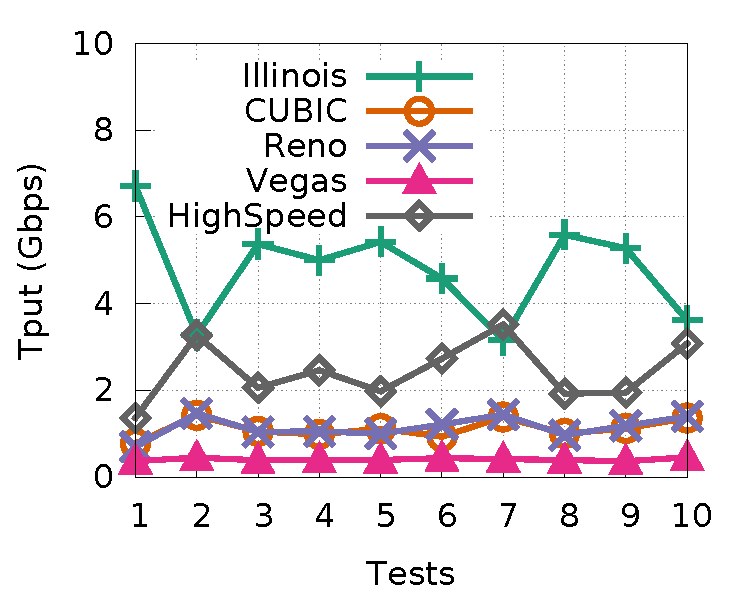
\includegraphics[width=\textwidth]{acdctcp/figures/tput_fairness/default_5CC_tput_detail.pdf}
		\caption{5 different CCs.}
                \label{unfairness_5CC}
        \end{subfigure}
        \begin{subfigure}[b]{0.225\textwidth}
                \centering
                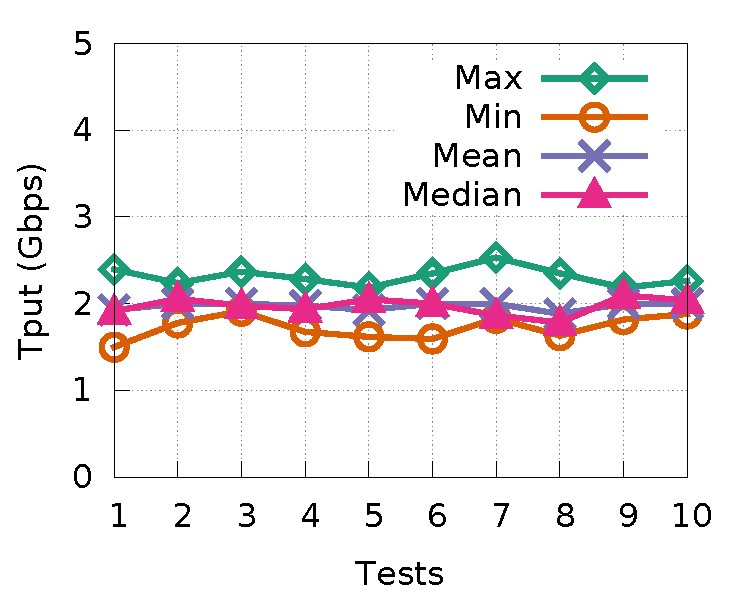
\includegraphics[width=\textwidth]{acdctcp/figures/tput_fairness/default_all_cubic_tput.pdf}
                \caption{All CUBIC.}
                \label{unfairness_all_cubic}
        \end{subfigure}
%        \begin{subfigure}[b]{0.24\textwidth}
%                \centering
%                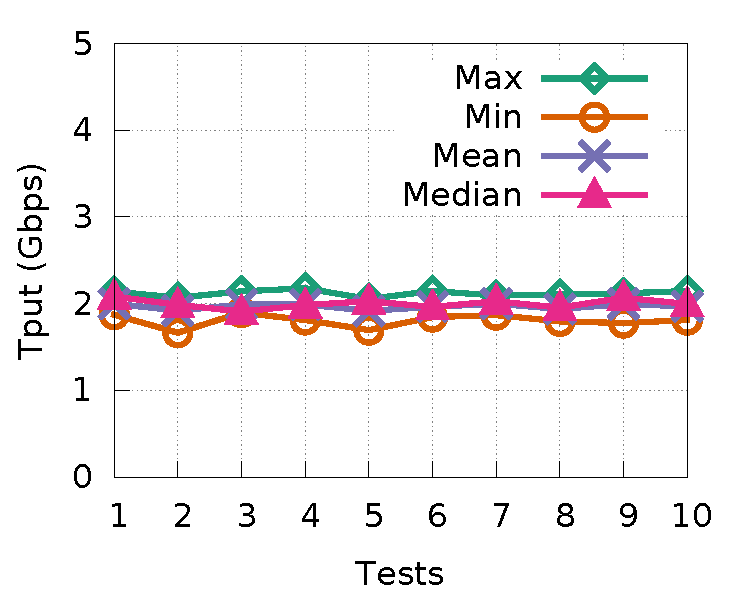
\includegraphics[width=\textwidth]{acdctcp/figures/tput_fairness/liquid_5CC_tput.pdf}
%                \caption{5 different CCs with \acdc{}.}
%                \label{fairness_5CC_with_ours}
%        \end{subfigure}
%        \begin{subfigure}[b]{0.24\textwidth}
%                \centering
%                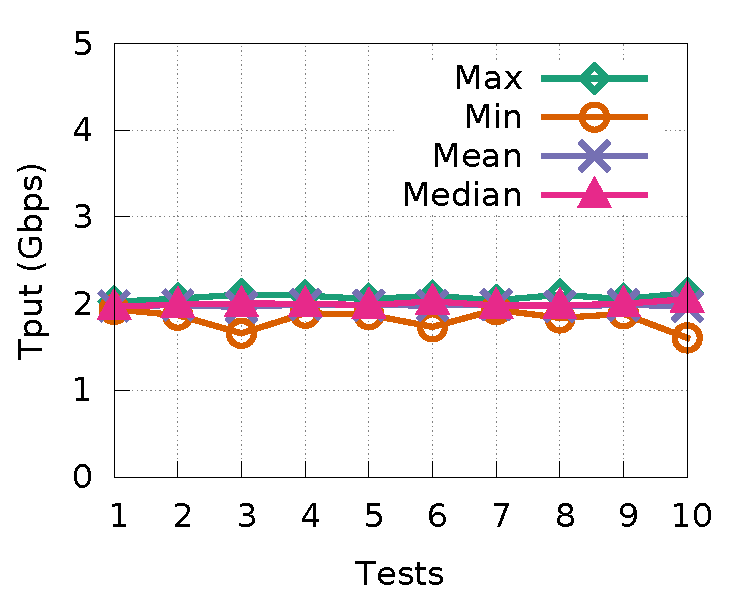
\includegraphics[width=\textwidth]{acdctcp/figures/tput_fairness/ecn_all_dctcp_tput.pdf}
%                \caption{All DCTCP.}
%                \label{fairness_5CC_with_dctcp}
%        \end{subfigure}
        \caption{Different congestion controls lead to unfairness.}
        \label{tput_unfair}
\end{figure}

The next benefit is~\acdc{} allows for {\em uniform}
congestion control to be implemented throughout the datacenter.
Unfairness arises when stacks are handled differently in the fabric or when conservative and aggressive
stacks coexist. Studies have shown ECN-capable and ECN-incapable flows do not exist gracefully on the
same fabric because packets belonging to ECN-incapable flows encounter severe packet drops when their packets
exceed queue thresholds~\cite{wu2012tuning,judd2015nsdi}. %Ideally, tenants shouldn't suffer based on such a simple configuration issue.
%~\eric{Do we have an argument that clients should be able to port their VMs to the cloud without making any changes
%or worrying about the low-level network details of the cloud provider?}
Additionally, stacks with different congestion control algorithms may not share the same fabric fairly.
For example, Figure~\ref{tput_unfair} shows the performance of five different TCP flows on the topology in
Figure~\ref{dumbbell_topology}. Each flow selects a congestion control algorithm available in Linux:
CUBIC~\cite{ha2008cubic}, Illinois~\cite{liu2008tcp}, HighSpeed~\cite{RFC3649},
New Reno~\cite{RFC3782} and Vegas~\cite{Brakmo1994}.
Figure~\ref{unfairness_5CC} shows aggressive stacks such as Illinois and HighSpeed
achieve higher bandwidth and thus fairness is worse than all flows using the
same stack (Figure~\ref{unfairness_all_cubic}). 
%A tenant should not be able
%to unfairly obtain higher bandwidth by simply changing its congestion control.

Another benefit of~\acdc{} is it allows for different congestion control algorithms to be assigned on
a per-flow basis. %Today, TCP congestion control is configured at an OS-level, so all of an OS's flows are forced to use the same congestion control algorithm.
A vSwitch-based approach can assign WAN flows to a congestion control algorithm that optimizes WAN performance~\cite{tan2006compound,flach2013reducing} and
datacenter flows to one that optimizes datacenter performance, even if these flows originate from the same VM (\eg{}, a webserver).
%This severely limits flexibility and forces tenants to optimize the performance of a subset of its flows. For example, a web server may choose a TCP stack to optimize
%WAN performance~\cite{tan2006compound,flach2013reducing} at the cost of harming back-end performance within the datacenter.~\eric{still need to clean}
Additionally, as shown in \cref{ss:cc-qos}, a flexible congestion control algorithm can provide relative bandwidth allocations to flows.
This is useful when tenants or administrators want to prioritize flows assigned to the same quality-of-service class.
In short, adjusting congestion control algorithms on a per-flow basis allows for 
enhanced flexibility and performance.
%As studies have shown that TCP can be optimized for datacenters~\cite{alizadeh2011data, stephens2014practical, wu2010ictcp,
%mittal2015timely, jose2015high}, WAN environments~\keqiang{cite Compound TCP?}, and even
%~\eric{one more example, wireless/60Ghz/free-space optics?}, selecting a per-flow TCP stack has the potential to
%enhance network performance. By moving congestion control to the vSwitch, administrators can assign a specific congestion control
%algorithm to each flow, optimizing the network performance of its clients in a seamless manner.~\eric{Also add QoS-based CC
%stuff here, since we have something.}

Finally, congestion control is not difficult to port. While the entire TCP stack may seem complicated and prone to high overhead,
the congestion control aspect of TCP is relatively light-weight and simple to implement. Indeed, studies
show most TCP overhead comes from buffer management~\cite{optimize-tcp-receive}, and
in our evaluation the computational overhead of~\acdc{} is less than one percentage point.
Porting is also made easy because congestion control implementations in Linux
are modular: DCTCP's congestion control resides in {\tt tcp\_dctcp.c} and is only about 350 lines of code. Given
the simplicity of congestion control, it is not hard to move its functionality to another
layer.
%~\crs{Furthermore,~\acdc{} does not rate limit or buffer packets, and our
%benchmarks show the computational overhead of~\acdc{} is less than one percentage point.}


\subsection{Tenant-Level Bandwidth Allocation}
%In addition to controlling congestion, public cloud administrators have to find ways to
%isolate the performance of different tenants and applications. 
\crs{While~\acdc{} enforces congestion control, transport layer schemes do not
provide fair bandwidth allocation among tenants because
a tenant with more concurrent flows can obtain
a higher share of bandwidth.
%The situation is further worsened by UDP flows since they are not subjected to any transport
%level congestion control.
In order to provide performance isolation in the network, datacenter operators can implement
a variety of bandwidth allocation schemes by either guaranteeing or proportionally
allocating bandwidth for tenants~\cite{rodrigues2011gatekeeper,Ballani2011oktopus,jeyakumar2013eyeq,shieh2011sharing,
Guo2010Secondnet,Popa2012Faircloud,Xie2012Proteus,Lam2012NetShare,jang2015silo}. 
%Simple static rate limiters enforced on many default public cloud images dictate an upper-bound on the bandwidth available
%to different classes of VMs.
% Congestion can occur when the cumulative bandwidth from a set of
%senders exceeds the bandwidth of a network link (incast is a special case). Consider the topology in Figure~\ref{dumbbell_topology},  
%with 5 flows traversing a bottleneck 10 Gbps link. Even in the case of a "perfect" allocation, where each flow is statically limited to 10 Gbps/5 flows = 2 Gbps,
%the latency caused by queueing heavily depends on the deployed TCP stack. We show this in Figure~\eric{cubic-fill}.
%CUBIC~\cite{ha2008cubic}, the default TCP congestion control algorithm in Linux, will aggressively fill
%the buffer of the congested output port, causing latencies to significantly increase. DCTCP, however, is able
%to keep buffers low~\cite{alizadeh2011data}, allowing for a queueing latency that is an order of magnitude lower than CUBIC's. These differences exist despite the fact
%that each scheme is able to achieve the same throughput over the congested link (Section~\ref{results}~\eric{Table 1}).
%Note that in Figure~\ref{cubic-fill}, DCTCP is run in the absence of a static rate limiter, meaning that it is effective
%in mitigating congestion's impact on latency. 
Some of these schemes share high-level architectural similarities to~\acdc{}.}
For example, EyeQ~\cite{jeyakumar2013eyeq} 
%provides a single dedicated switch abstraction for tenant VMs and 
handles bandwidth allocation at
the edge with a work-conserving distributed bandwidth arbitration scheme. It enforces
rate limits at senders based on feedback generated by receivers. Similarly, Seawall~\cite{shieh2011sharing}
provides proportional bandwidth allocation to a VM or application by forcing all
traffic through a congestion-controlled tunnel configured through weights and endpoint feedback.


The fundamental difference between these schemes and our approach is the design
goals determine the granularity on which they operate. 
Performance isolation schemes generally focus on {\em bandwidth allocation on a VM-level} and
are not sufficient to relieve the network of congestion because they do not
operate on flow-level granularity. 
For example, the single switch abstraction
in EyeQ~\cite{jeyakumar2013eyeq} and Gatekeeper~\cite{rodrigues2011gatekeeper} explicitly assumes a congestion-free 
fabric for optimal bandwidth allocation between pairs of VMs. This abstraction doesn't hold in multi-pathed
topologies when failure, traffic patterns or ECMP hash collisions~\cite{al2010hedera} cause congestion in the core.
Communication between a pair of VMs may consist of
multiple flows, each of which may traverse a distinct path. Therefore,
enforcing rate limits on a VM-to-VM level is too coarse-grained to determine how specific flows should adapt in
order to mitigate the impact of congestion on their paths. Furthermore, a scheme like Seawall~\cite{shieh2011sharing}
cannot be easily applied to flow-level granularity because
its rate limiters are unlikely to scale in the number of flows at high networking speeds~\cite{radhakrishnan2014senic}
and its allocation scheme does not run at fine-grained round-trip
timescales required for effective congestion control. Additionally, Seawall violates our design
principle by requiring VM modifications to implement congestion-controlled tunnels.

%Three bandwidth allocation schemes, EyeQ~\cite{jeyakumar2013eyeq}, Gatekeeper~\cite{rodrigues2011gatekeeper} and Seawall~\cite{shieh2011sharing}
%use congestion control techniques to provide bandwidth guarentees. At a high-level, these schemes employ
%VM-to-VM tunnels that partition bandwidth at the network edge (EyeQ) or proportionally allocate bandwidth
%over network links (Seawall). In addition, both EyeQ and Seawall are designed to adapt to network congestion
%by analyzing the fraction of packets marked with ECN bits to adjust the rates imposed on the VM-to-VM tunnels. 
%VM-to-VM tunnels are not fine-grained enough to effective mitigate queueing latencies caused by congestion.
%For example, datacenter topologies typically contain multiple paths from a source to a destination. Therefore,
%if a VM has multiple flows to another VM, those flows may take seperate paths (thanks to ECMP). By combining all flows
%over a single logical VM-to-VM tunnel, the proportion of packets experiencing congestion gets muddled. Flows that
%are not experiencing any congestion get their rates reduced unneccesarrily. Flows that are experiencing congestion
%do not reduce their rates fast enough.~\eric{i know this needs work} 

%\eric{Seawall talk mentioned O($10^5$) new tasks per minute. Can we make something more concrete above?}


\begin{figure}[!t]
        \centering
  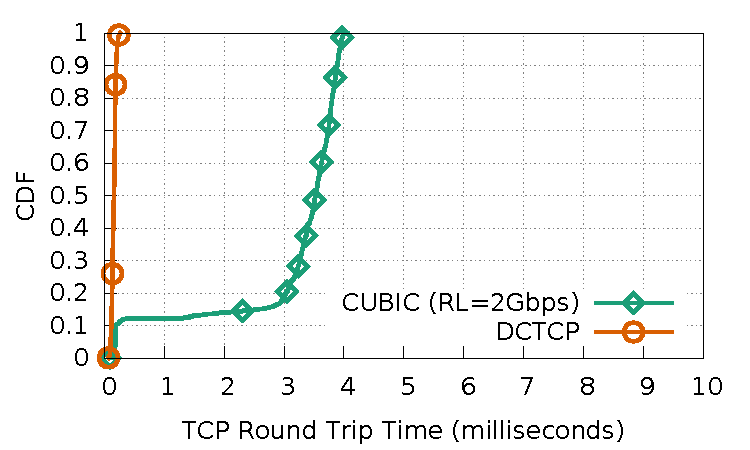
\includegraphics[width=0.45\textwidth]{acdctcp/figures/motivation/motivation_2Gbps_cubic_rl_dctcp_sockperf.pdf}
        \caption{CDF of RTTs showing CUBIC fills buffers.}
        \label{cubic-fill}
\end{figure}
%\subsection{Bandwidth Allocation with Transport Control}
%In fact, bandwidth allocation schemes attempt to provide tenant level performance isolation
%regardless of the tenant transport stack and protocol, even though the stack has a large impact on congestion. 
~\crs{The above points are not intended to criticize any given work, but rather support the argument that
it is important for a cloud provider to enforce {\em both} congestion control and bandwidth allocation.
Congestion control can ensure low latency and high utilization, and
bandwidth allocation can provide tenant-level fairness.}
Bandwidth allocation schemes alone are insufficient to mitigate congestion because certain TCP stacks aggressively
fill switch buffers. Consider a simple example where five flows send simultaneously
on the 10 Gbps topology in Figure~\ref{dumbbell_topology}. Even when the bandwidth is allocated "perfectly"
at 2 Gbps per flow, CUBIC saturates the output port's buffer and leads to inflated round-trip times (RTTs) for traffic
sharing the same link.
%~\footnote{Note the servers are not over-subscribed in this scenario, so even
%bounding rate limiters to 10 Gbps may be deemed satisfactory by some edge-based bandwidth allocation schemes.}. 
Figure~\ref{cubic-fill} shows these RTTs for CUBIC and also DCTCP, 
which is able to keep queueing latencies, and thus RTTs, low even though no rate limiting was applied.
Therefore, it is important for cloud providers to exercise a desired congestion
control.

In summary, our vision regards enforcing tenant congestion control and bandwidth allocation as {\em complimentary} and we claim 
an administrator should be able to
combine any congestion control (\eg{}, DCTCP) with any bandwidth allocation scheme (\eg{}, EyeQ). 
Flow-level congestion control and tenant performance isolation need not be solved by the same scheme,
so~\acdc{}'s design goal is to be modular in nature so it can co-exist with any bandwidth allocation scheme
and its associated rate limiter (and also in the absence of both). 
%To the best of our knowledge,~\acdc{} is the first work that advocates moving flow-level transport congestion control
%out of the VM and into the hypervisor.~\eric{keep?}

%~\eric{is this fair in respect to seawall? and what about NICs that support full TCP offload?}
%A key design goal of~\acdc{} is for it to be modular in nature so it can co-exist with any bandwidth allocation scheme 
%and its associated rate-limiter (and also in the absence of both).
%In order to achieve this goal,~\acdc{} satisfies a variety of constraints. First, it is
%computationally light-weight in order to minimize the overhead of its adoption. Second,
%it doesn't require any changes to VMs or network hardware so it can be deployed in
%current and future networks. Third, our scheme works in the absence of specific topology
%information and works over arbitrary topologies. Fourth, it does not require
%any information about tenant traffic patterns or require specific VM placement or admission
%mechanisms.
%

\section{Design}
\label{design}
\begin{figure}[!t]
        \centering
  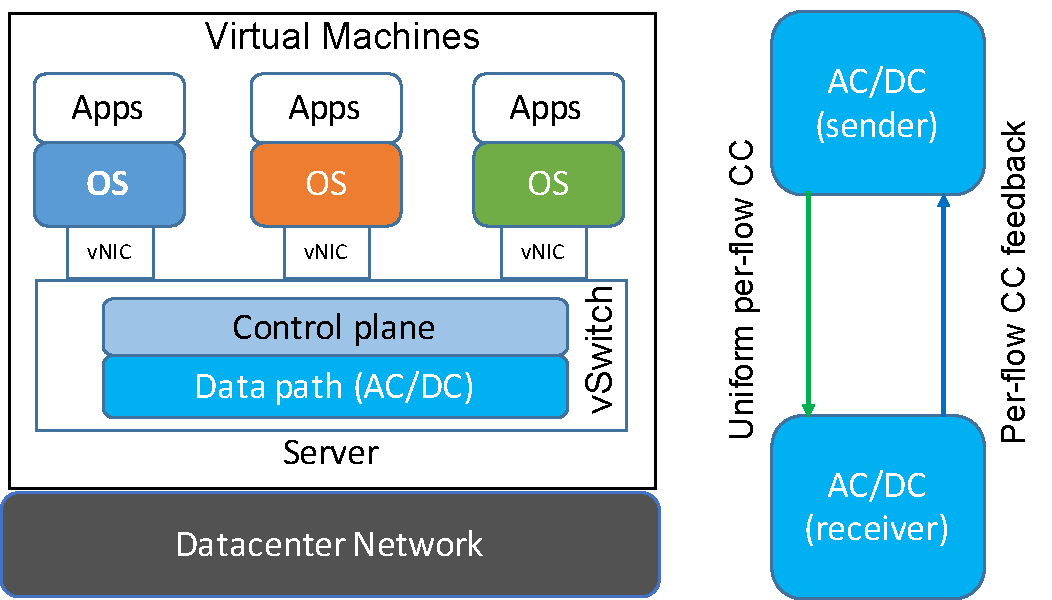
\includegraphics[width=0.5\textwidth]{acdctcp/figures/acdc_highlevel.pdf}
        \caption{\acdc{} high-level architecture.}
        \label{acdc_highlevel}
\end{figure}

This section provides an overview of~\acdc{}'s design. First, we show how basic
congestion control state can be inferred in the vSwitch. Then we study
how to implement DCTCP. Finally, we discuss how to enforce congestion
control in the vSwitch and provide a brief overview of how per-flow differentiation
can be implemented.


\begin{figure}[th]
        \centering
  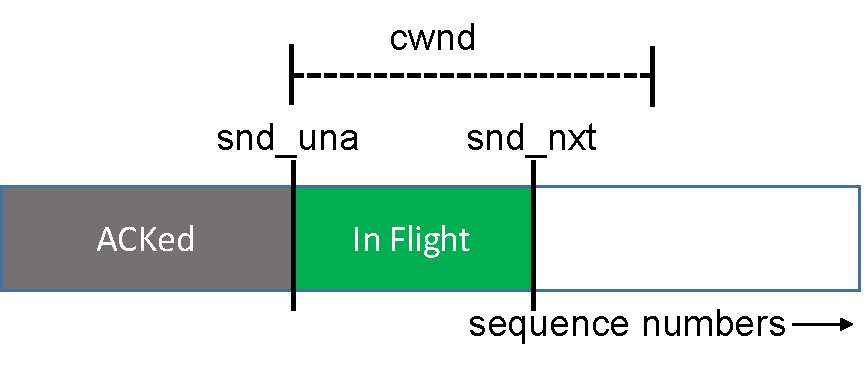
\includegraphics[width=0.5\textwidth]{acdctcp/figures/tcp-state-new.pdf}
        \caption{Variables for TCP sequence number space.}
        \label{tcpstate}
\end{figure}
\subsection{Obtaining Congestion Control State}
\label{ss:tcpstate}
Figure~\ref{acdc_highlevel} shows the high-level structure of \acdc{}. Since it is
implemented in the datapath of the vSwitch, all traffic can be monitored. The sender
and receiver modules work together to implement per-flow congestion control (CC).

We first demonstrate how congestion control state can be inferred.
Figure~\ref{tcpstate} provides a visual of the TCP sequence number space. The {\tt snd\_una} variable is the first byte
that has been sent, but not yet ACKed. The {\tt snd\_nxt} variable is the 
next byte to be sent. Bytes between {\tt snd\_una} and {\tt snd\_nxt} are in flight.
The largest number of packets that can be sent and unacknowledged is bounded by \cwnd{}.
{\tt snd\_una} is simple to update: each ACK contains an acknowledgement number ({\tt ack\_seq}), and 
{\tt snd\_una} is updated when {\tt ack\_seq} $>$ {\tt snd\_una}.
When packets traverse the vSwitch from the VM, {\tt snd\_nxt} is updated if the sequence
number is larger than the current {\tt snd\_nxt} value.
Detecting loss is also relatively simple. If {\tt ack\_seq $\le$ snd\_una}, then
a local {\tt dupack} counter is updated. Timeouts can be inferred when {\tt snd\_una $<$ snd\_nxt}
and an inactivity timer fires. The initial~\cwnd{} is set to a default value of 10~\cite{RFC6928}. 
With this state, the vSwitch can determine appropriate~\cwnd{} values for canonical
TCP congestion control schemes.
%More advanced congestion control techniques that rely on timestamps, round-trip times, SACKs or 
%FACKs can also be implemented. 
We omit additional details in the interest of space. 



\subsection{Implementing DCTCP}
%\begin{figure}[!t]
%        \centering
%  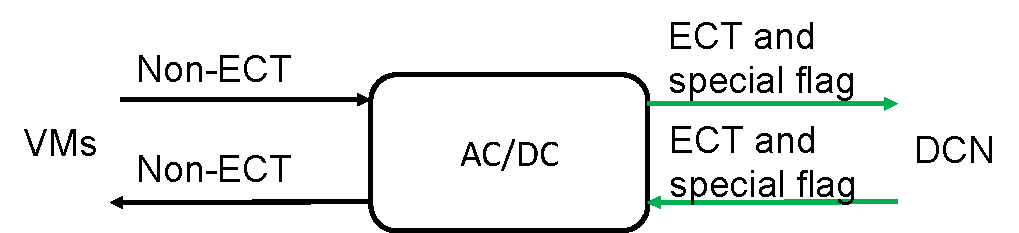
\includegraphics[width=0.45\textwidth]{acdctcp/figures/acdc_ECT_marking.pdf}
%        \caption{Simple stateless ECT marking in \acdc{}. 
%		Turn all intra-DC TCP packets in the fabric into ECT.}
%        \label{acdc_ect_marking}
%\end{figure}

%\begin{figure}[!t]
%        \centering
%  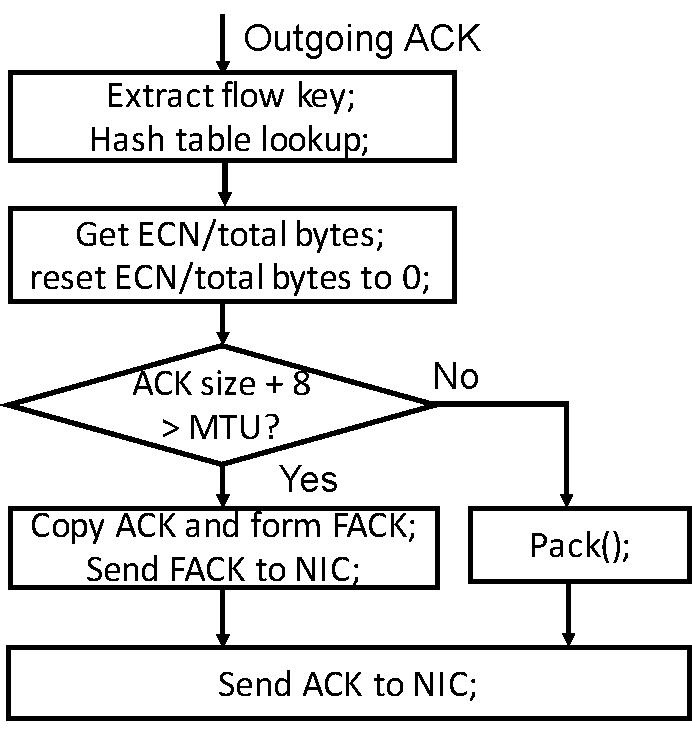
\includegraphics[width=0.25\textwidth]{acdctcp/figures/carry_ecn_info.pdf}
%        \caption{Carrying the congestion information back. 
%		Being compatible with TSO and minimizing CPU and traffic overhead.}
%        \label{acdc_carry_ecn_info}
%\end{figure}

This section discusses how to obtain DCTCP state and perform its congestion control.


\tightparagraph{ECN marking} 
DCTCP requires flows to be ECN-capable, but the VM's TCP stack may not support ECN.
Thus, all egress packets are marked to be ECN-capable on the sender module. 
When the VM's TCP stack does not support ECN, all ECN-related bits on ingress packets are stripped at the sender
and receiver modules in order to preserve the original TCP settings. When the VM's TCP
stack does support ECN, the~\acdc{} modules strip the {\tt congestion encountered} 
bits in order to prevent the VM's TCP stack from decreasing rates too aggressively
(recall DCTCP adjusts~\cwnd{} proportional to the fraction of congested packets, while traditional schemes conservatively reduce~\cwnd{} by half). A reserved bit in
the header is used to determine if the VM's TCP stack originally 
supported ECN.
%Algorithm~\ref{alg:non-ect-to-ect} changes non-ECT packets into ECT packets
%in the virtual switch before the packets enter the fabric and
%change them back when they arrive at the destination virtual switch.
%$p.pretendECT$ is set or cleared by flipping the 2nd bit of the 3 reserved bits in TCP header.
%After applying this algorithm, all TCP packets traversing the network appear to be ECT packets.
%So the ECT and non-ECT coexistence issue is solved.
%Also, because we change non-ECT back at the destination virtual switch,
%so TCP is not aware of such a transformation and \acdc{} does not break any TCP connections or applications.
%Algorithm~\ref{alg:non-ect-to-ect} leverages hardware checksumming feature in the NIC implicitly to reduce CPU overhead.
%\todo{how to add comment in this algorithm?}.
%
%
%\begin{algorithm}[t]
%\caption{ECT marking in \acdc{}}
%\label{alg:non-ect-to-ect}
%\begin{algorithmic}[1]
%%\STATE \Comment{packet $p$ is TCP packet}
%\IF{$p$ is going to the network}
%\IF{$p$ is non-ECT}
%\STATE change $p$ to ECT by modifying IP header
%\STATE set $p.pretendECT$
%%\STATE set the 2nd bit of the 3 reserved bits in TCP header to 1
%\ENDIF
%\ELSIF{$p$ is coming from the network}
%\IF{$p$ is non-ECT and $p.pretendECT$ is set}
%\STATE change $p$ back to non-ECT by modifying IP header
%\STATE clear $p.pretendECT$
%%\STATE clear the 2nd bit of the reserved bits
%\ENDIF
%\ENDIF
%\end{algorithmic}
%\end{algorithm}
%

\tightparagraph{Obtaining ECN feedback}
In DCTCP, the fraction of packets experiencing congestion needs to be reported to the sender. 
%DCTCP relays this information from the destination to the sender by essentially modulating data
%in the ACK reporting scheme. Sender and receiver agree on an ACK state-machine that effectively 
%communicates how many packets were received with ECN vs how many were not. Because the TCP stack
%in the VM may not be DCTCP, we do not want to rely on the ACK modulation scheme. 
Since the VM's TCP stack may not support ECN, the~\acdc{} receiver module monitors
the total and ECN-marked bytes received for a flow. Receivers piggy-back the
reported totals on ACKs by adding an additional 8 bytes as a TCP Option. This is called 
a Piggy-backed ACK (PACK). The PACK is created by moving the IP and TCP headers into
the ACK packet's {\tt skb} headroom~\cite{kernel-skb}. The totals are inserted into the vacated space and the memory
consumed by the rest of the packet (\ie{}, the payload) is left as is. The IP header checksum, IP packet length and TCP Data Offset fields are recomputed and the 
TCP checksum is calculated by the NIC. The PACK option is stripped at the
sender so it is not exposed to the VM's TCP stack. 

If adding a PACK creates a packet larger than the MTU, the NIC offload feature (\ie{}, TSO)
will replicate the feedback information over multiple packets, which skews the feedback.
Therefore, a dedicated feedback packet called a Fake ACK (FACK) is sent when the MTU
will be violated. The FACK is sent in addition to the real TCP ACK.
FACKs are also discarded by the sender after logging the included
data. In practice, most feedback takes the form of PACKs.

%
%\begin{algorithm}[t]
%\caption{Carrying the congestion information back}
%\label{alg:outgoing}
%\begin{algorithmic}[1]
%%\STATE flow\_key $\leftarrow$ \{dstip, srcip, dstport, srcport\}
%%\STATE ack\_entry $\leftarrow$ rcv\_ack\_hashtbl\_lookup(flow\_key)
%%\STATE end\_seq $\leftarrow$ ntohl(tcp.seq) + tcp.data\_len
%%\IF{after(end\_seq, ack\_entry.snd\_nxt)}
%%       \STATE ack\_entry.snd\_nxt $\leftarrow$ end\_seq
%%\ENDIF
%%\IF{tcp.ack}
%\IF{outgoing skb is a TCP ACK}
%\STATE flow\_key $\leftarrow$ \{dstip, srcip, dstport, srcport\}
%\STATE entry $\leftarrow$ rcv\_data\_hashtbl\_lookup(flow\_key)
%        \IF{entry.total\_bytes > 0}
%                \STATE ecn\_bytes $\leftarrow$ entry.ecn\_bytes
%                \STATE total\_bytes $\leftarrow$ entry.total\_bytes
%                \STATE entry.ecn\_bytes $\leftarrow$ 0
%                \STATE entry.total\_bytes $\leftarrow$ 0
%        \ENDIF
%        \IF{total\_bytes > 0}
%                \IF{skb.data\_len < (MTU -- HEADROOM)}
%                        \STATE skb $\leftarrow$ ovs\_pack(skb, ecn\_bytes, total\_bytes)
%                \ELSE
%                        \STATE fack $\leftarrow$ ovs\_fack(skb, ecn\_bytes, total\_bytes)
%                \ENDIF
%        \ENDIF
%\ENDIF
%\IF{fack != NULL}
%        \STATE sendtoNIC(fack)
%\ENDIF
%\STATE sendtoNIC(skb)
%\end{algorithmic}
%\end{algorithm}
%

\begin{figure}[!t]
        \centering
  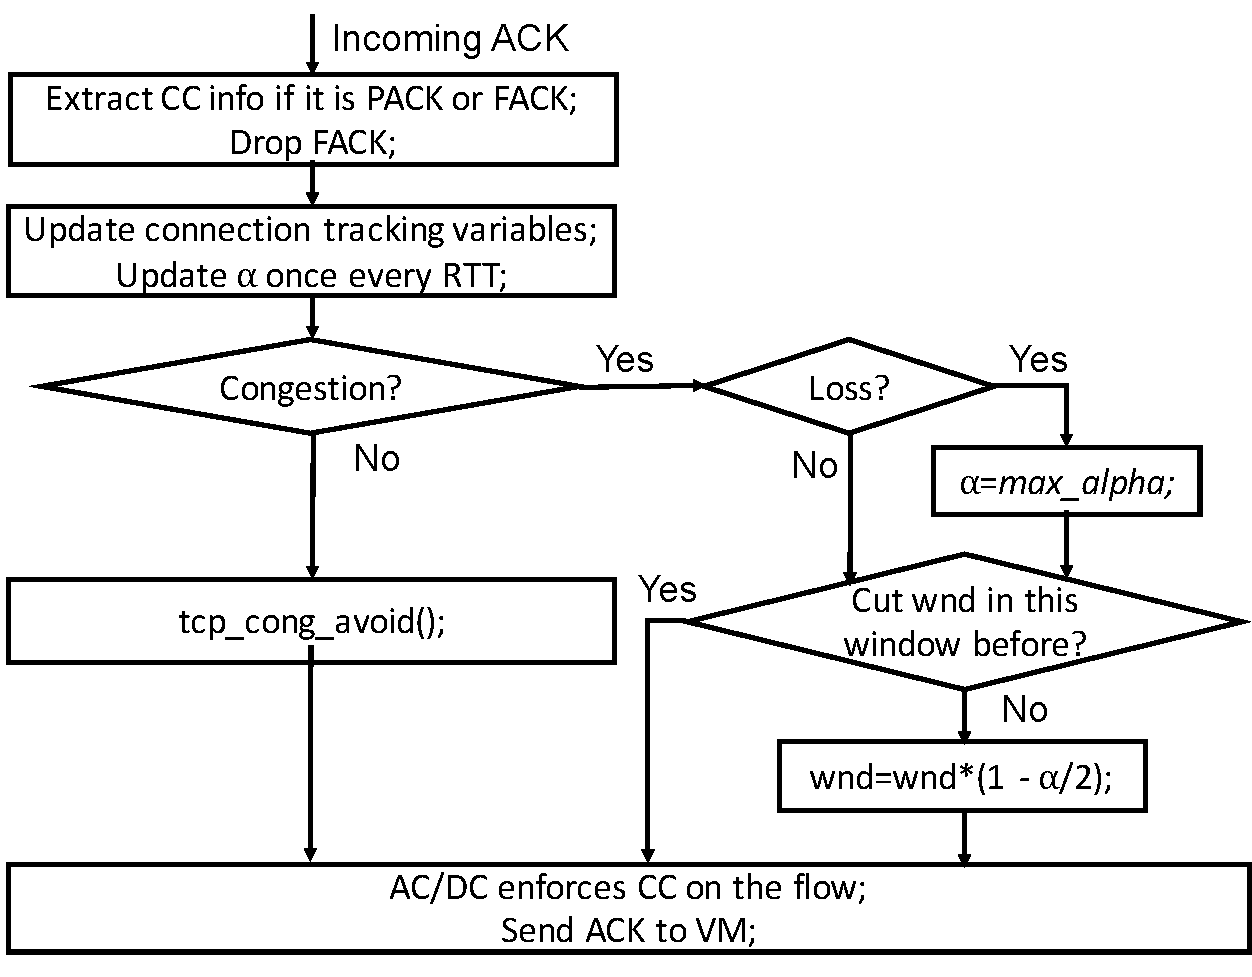
\includegraphics[width=0.49\textwidth]{acdctcp/figures/acdc_cc.pdf}
        \caption{DCTCP congestion control in \acdc{}.}
        \label{acdc_cc}
\end{figure}
\tightparagraph{DCTCP congestion control} 
Once the fraction of ECN-marked packets is obtained, implementing DCTCP's logic is straightforward.
Figure~\ref{acdc_cc} shows the high-level design. 
First, congestion control (CC) information is extracted from FACKs and PACKs. Connection tracking
variables (described in \cref{ss:tcpstate}) are updated based on the ACK. The variable
$\alpha$ is an EWMA of the fraction of packets that experienced congestion and is updated roughly
once per RTT. If congestion was not encountered (no loss or ECN), then {\tt tcp\_cong\_avoid} advances~\cwnd{}
based on TCP New Reno's algorithm, using slow start or congestion avoidance as needed. If congestion was
experienced, then~\cwnd{} must be reduced. DCTCP's instructions indicate the window should
be cut at most once per RTT.
Our implementation closely tracks the Linux source code, and
additional details can be referenced externally~\cite{alizadeh2011data,ietf-tcpm-dctcp}.


%\begin{algorithm}[!tbh]
%\caption{Congestion control in \acdc{}}
%\label{alg:incoming}
%\begin{algorithmic}[1]
%\IF{incoming skb is a TCP ACK}
%\STATE initialize is\_rack, is\_pack and is\_fack
%\STATE flow\_key $\leftarrow$ \{srcip, dstip, srcport, dstport\}
%\STATE entry $\leftarrow$ rcv\_ack\_hashtbl\_lookup(flow\_key)
%\IF{is\_pack or is\_fack}
%        \STATE unpack and extract ecn\_bytes and total\_bytes
%        \STATE update(entry.ecn\_bytes, ecn\_bytes)
%        \STATE update(entry.total\_bytes, total\_bytes)
%\ENDIF
%\IF{is\_rack or is\_pack}
%        \STATE acked $\leftarrow$ tcp.ack\_seq -- entry.snd\_una
%        \STATE entry.snd\_una $\leftarrow$ tcp.ack\_seq
%        \IF{duplicated ACK}
%                \STATE entry.dupack\_cnt++
%        \ENDIF
%        \STATE dctcp\_update\_alpha(entry)
%        \IF{acked > 0}
%                \IF{may\_raise\_rwnd(entry)}
%                        \STATE tcp\_cong\_avoid(entry, acked)
%                \ENDIF
%        \ENDIF
%\ENDIF
%\IF{entry.dupack\_cnt >= 3 or ecn\_bytes > 0}
%        \IF{entry.dupack\_cnt >= 3}
%                \STATE entry.alpha $\leftarrow$ MAX\_ALPHA
%                \STATE entry.loss $\leftarrow$ true
%        \ENDIF
%        \IF{may\_reduce\_rwnd(entry)}
%                \STATE entry.ssthresh $\leftarrow$ dctcp\_ssthresh(ack\_entry)
%                \STATE entry.rwnd $\leftarrow$ min(RWND\_MIN, entry.ssthresh)
%                \STATE entry.reduced $\leftarrow$ true
%        \ENDIF
%\ENDIF
%\IF{is\_rack or is\_pack}
%        \STATE tcp.window $\leftarrow$ min(tcp.window, entry.rwnd)
%\ENDIF
%\IF{is\_fack}
%        \STATE drop(skb)
%\ENDIF
%\ENDIF
%\end{algorithmic}
%\end{algorithm}
%

\subsection{Enforcing Congestion Control}
\label{ss:enforce}
There must be a mechanism to ensure a VM's TCP flow adheres to the~\cwnd{} determined in the vSwitch.
Luckily, TCP provides built-in functionality that can be reprovisioned for~\acdc{}. Specifically,
TCP's flow control allows a receiver to advertise the amount of data it is willing to process via
a receive window (\rwnd{}).~\crs{Similar to other works~\cite{Kalampoukas02,Spring00}, the vSwitch overwrites~\rwnd{} with its calculated~\cwnd{}}.
In order to preserve TCP semantics, this value is overwritten only when it is smaller than the packet's original~\rwnd{}.
The VM's flow then uses $min(\cwnd{},\rwnd{})$ to limit how many packets it can send.

This enforcement scheme must be compatible with TCP receive window scaling to work in practice.
Scaling ensures~\rwnd{} does not become an unnecessary upper-bound in high bandwidth-delay networks
and provides a mechanism to left-shift~\rwnd by a window scaling factor~\cite{RFC1323}. 
The window scaling factor is negotiated during TCP's handshake, so~\acdc{} monitors handshakes
to obtain this value. Calculated congestion windows are adjusted accordingly.
TCP receive window auto-tuning~\cite{semke1998automatic} manages buffer state
and thus is an orthogonal scheme~\acdc{} can safely ignore.

Ensuring a VM's flow adheres to~\rwnd{} is relatively simple. The vSwitch calculates a new congestion 
window every time an ACK is received. This value provides a bound on the number of bytes the VM's flow
is now able to send. VMs with unaltered TCP stacks will naturally follow our enforcement scheme because the stacks
will simply follow the standard. Flows that circumvent the standard can be policed by dropping
excess packets not allowed by the calculated congestion window, which incentivizes tenants to respect the standard.

While simple, this scheme provides a surprising amount of flexibility. For example, TCP enables
a receiver to send a TCP Window Update to update~\rwnd{}~\cite{RFC5681}.~\acdc{}
can create these packets to update windows without relying on ACKs.
Additionally, the sender module can generate duplicate ACKs to to trigger retransmissions. This is useful when 
the VM's TCP stack has a larger timeout value than~\acdc{} (\eg{}, small timeout values
have been recommended for incast~\cite{vasudevan2009safe}). 
%In this case, the vSwitch can send three dup-ACKs (with
%an appropiate~\rwnd{}) to trigger the VM's TCP flow to retransmit.
% EJR-- put back in for camera ready?
\crs{
Another useful feature is when~\acdc{} allows a TCP stack to send {\em more} data. This can occur when
a VM TCP flow aggressively reduces its window when ECN feedback is received. By removing ECN feedback
in~\acdc{}, the VM TCP stack won't reduce~\cwnd{}. 
In a similar manner, DCTCP limits loss more effectively than aggressive TCP stacks. Without loss
or ECN feedback, VM TCP stacks grow~\cwnd{}. This causes~\acdc{}'s~\rwnd{} to become the limiting window, and thus~\acdc{} can 
increase a flow's rate instantly when~\rwnd{} $<$ \cwnd{}. Note, however,~\acdc{} cannot force
a connection to send more data than the VM's~\cwnd{} allows.
}

Another benefit of~\acdc{} is that it scales in the number of flows.
Traditional software-based rate limiting schemes, like Linux's Hierarchical Token Bucket, 
incur high overhead due to frequent interrupts and contention~\cite{radhakrishnan2014senic} and
therefore do not scale gracefully. NIC or switch-based rate limiters are low-overhead, but typically
only provide a handful of queues. Our enforcement algorithm does not rate limit or buffer packets because it exploits TCP
flow control. Therefore, rate limiting schemes can be used at a coarser granularity (\eg{}, VM-level).


~\crs{
Finally, we outline~\acdc{}'s limitations. 
Since~\acdc{} relies on sniffing traffic, schemes that encrypt TCP headers (\eg{}, IPSec) are not supported. Our implementation only supports TCP, but we believe it can be extended to handle UDP similar to
prior schemes~\cite{shieh2011sharing,jeyakumar2013eyeq}.
Implementing per-flow DCTCP-friendly UDP tunnels and studying its impact remains future work, however. And finally, 
while MPTCP supports per-subflow~\rwnd{}~\cite{RFC6824}, it is not included in our case study and a more detailed analysis
is future work.
}
 


%\tightparagraph{Compatible with receive window auto-tuning and window scaling}
%TCP receive window auto-tuning~\cite{semke1998automatic,receive-auto-runing} is a commonly used feature 
%in modern TCP stacks. It is enabled by default in recent Linux and Windows distributions.
%Receive window auto-tuning was proposed to automatically 
%set socket buffer size based on network conditions to 
%improve network performance while optimizing the memory usage by TCP connections.
%Because \acdc{} overwrites the real \rwnd{} value embedded in TCP ACK header 
%only when \acdc{}'s running \rwnd{} is smaller than 
%the real \rwnd{}, thus \acdc{} does not break the correctness of TCP semantics 
%and is compatible with receive window auto-tuning.
%

\begin{figure}[t]
        \centering
        \begin{subfigure}[b]{0.45\textwidth}
                \centering
                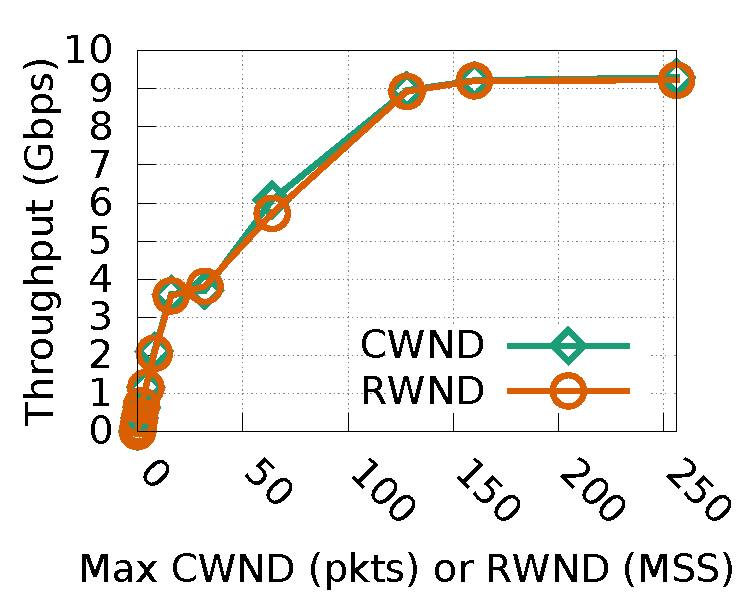
\includegraphics[width=\textwidth]{acdctcp/figures/new_enforce/new_tput_cwnd_rwnd_cubic_15k.pdf}
                \caption{MTU = 1.5KB.}
                \label{effectiveness_15k}
        \end{subfigure}
        \begin{subfigure}[b]{0.45\textwidth}
                \centering
                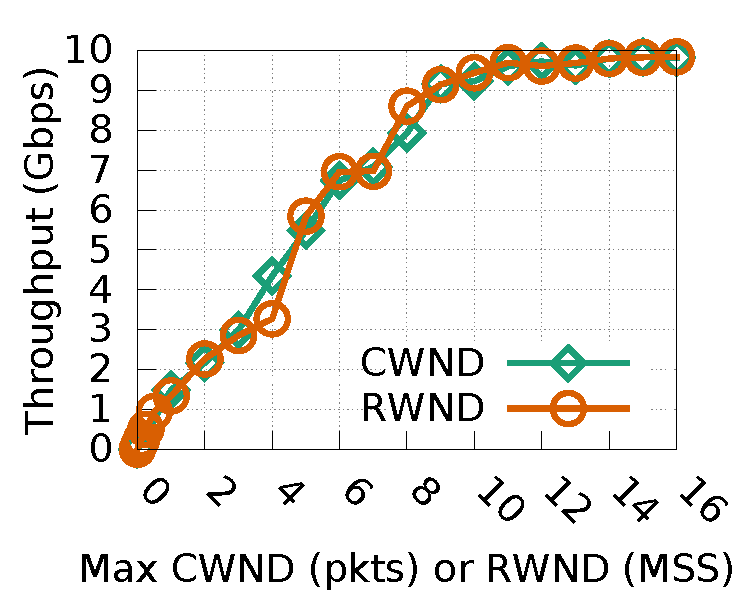
\includegraphics[width=\textwidth]{acdctcp/figures/new_enforce/new_tput_cwnd_rwnd_cubic_9k.pdf}
                \caption{MTU = 9KB.}
                \label{effectiveness_9k}
        \end{subfigure}
        \caption{Using \rwnd{} can effectively control throughput.}
                %Experiments are conducted on a 10G testbed. TCP CUBIC but New Reno shows similar results.
                %Linux 3.18.0. We control maximal \rwnd{} value by modifying the receiver's advertised window size in TCP ACKs
                %in the Open vSwitch. We control maximal \cwnd{} by specifying ``snd\_cwnd\_clamp" value in Linux TCP.}
        \label{rwnd_effectiveness}
\end{figure}
\subsection{Per-flow Differentiation}
\label{ss:cc-qos}
\acdc{} can assign different congestion control algorithms
on a per-flow basis. This gives administrators additional flexibility and control by 
assigning flows to specific congestion control algorithms based on policy.
For example, flows destined to the WAN may be assigned CUBIC and flows destined within the
datacenter may be set to DCTCP. 

Administrators can also enable per-flow bandwidth allocation schemes.
A simple scheme enforces an upper-bound
on a flow's bandwidth. Traditionally, an upper-bound on a flow's~\cwnd{} can be
specified by {\tt snd\_cwnd\_clamp} in Linux.~\acdc{} can provide similar functionality
by bounding~\rwnd{}. Figure~\ref{rwnd_effectiveness} shows the behavior is equivalent. This 
graph can also be used to convert a desired upper-bound on bandwidth into an appropriate maximum~\rwnd{} (the
graph is created on an uncongested link to provide a lower bound on RTT). 

In a similar fashion, administrators can assign different bandwidth priorities to flows by altering the 
congestion control algorithm. Providing differentiated services via congestion control has 
been studied~\cite{Venkataramani2002tcpnice,shieh2011sharing}. Such schemes are useful because networks
typically contain only a limited number of service classes and bandwidth may need to be allocated on
a finer-granularity. We propose a unique priority-based congestion control algorithm for~\acdc{}.
Specifically, DCTCP's congestion control algorithm is modified to incorporate a priority, $\beta \in [0,1]$:
\begin{equation}
rwnd = rwnd (1 - (\alpha - \frac{\alpha{}\beta}{2}))
\label{eqn:cc-qos}
\end{equation}
Higher values of $\beta$ give higher priority. 
When $\beta{}=1$, Equation~\ref{eqn:cc-qos} simply converts to DCTCP congestion control. When
$\beta{}=0$, flows aggressively back-off (\rwnd{} is bounded by 1 MSS to avoid starvation). This equation
alters multiplicative decrease instead of additive increase because increasing~\rwnd{} 
cannot guarantee the VM flow's~\cwnd{} will allow the flow to increase its sending rate.

%subsection{How to keep low overhead?}
%Move to Implementation?
%Connection tracking~\cite{ayuso2006netfilter,ovs-conntrack}.
%
%\subsection{How is it complimentary to other schemes?}
%Like bandwidth allocation.
%
%~\eric{Should we talk about how we can actually increase rate of VM TCP?}
%


%In history, TCP used packet loss as the signal of network congestion. 
%But, using packet loss as the signal can not meet the performance demand of datacenter environment 
%due to high queueing latency and frequent packet losses. Packet loss-based congestion control 
%can work reasonably well for large data transfers but does harm time-critical RPCs. 
%Thus, new congestion control algorithms designed for datacenter networks were proposed. 
%They can be classified into 2 categories: Explicit Congestion Notification (ECN)-based and 
%latency-based. The most straightforward way is to treat ECN as packet loss and cut congestion 
%window before network queue built up and packet loss happens---but this can harm flow throughput. 
%DCTCP improves this by cut window properly based on the portion of marked packets and 
%gives high throughput for large flows and low latency for mice flows. 
%Latency-based congestion control such as TCP-NV, TIMELY, DX use the end-to-end latency 
%as the signal of network congestion. Compared with ECN-based approach, latency is a more 
%prevalent signal for congestion (i.e., does not need ECN capability on the switches). 
%But the challenge of such approaches is to find ways to combat with latency measurement noise 
%caused by TSO, LRO and interrupt coalescence.
%


%\begin{figure}[t]
%        \centering
%        \begin{subfigure}[b]{0.225\textwidth}
%                \centering
%                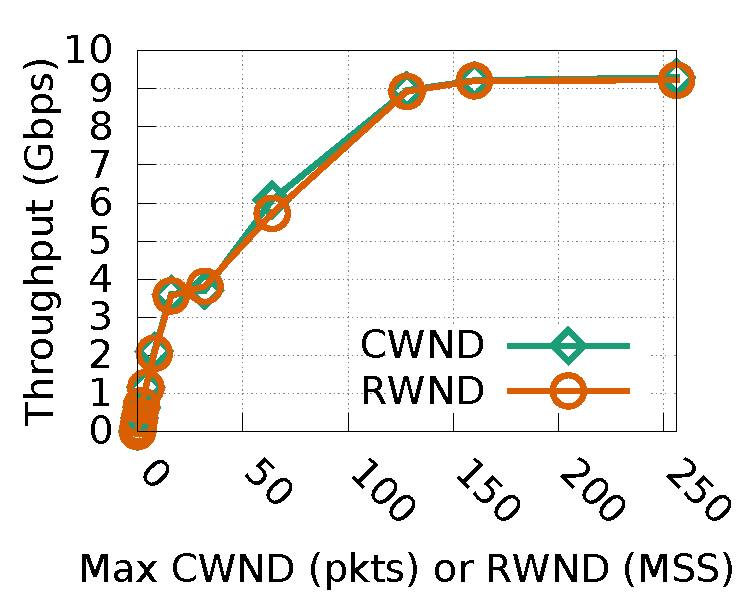
\includegraphics[width=\textwidth]{acdctcp/figures/new_enforce/new_tput_cwnd_rwnd_cubic_15k.pdf}
%                \caption{MTU = 1.5KB.}
%                \label{effectiveness_15k}
%        \end{subfigure}
%        \begin{subfigure}[b]{0.225\textwidth}
%                \centering
%                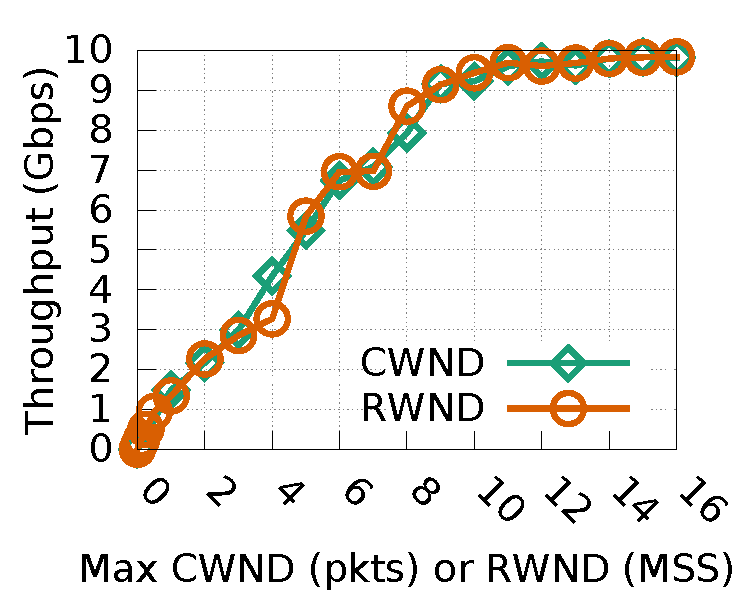
\includegraphics[width=\textwidth]{acdctcp/figures/new_enforce/new_tput_cwnd_rwnd_cubic_9k.pdf}
%                \caption{MTU = 9KB.}
%                \label{effectiveness_9k}
%        \end{subfigure}
%        \caption{Using \rwnd{} can effectively control throughput. 
%		Experiments are conducted on a 10G testbed. TCP CUBIC but New Reno shows similar results.
%		Linux 3.18.0. We control maximal \rwnd{} value by modifying the receiver's advertised window size in TCP ACKs
%		in the Open vSwitch. We control maximal \cwnd{} by specifying ``snd\_cwnd\_clamp" value in Linux TCP.}
%        \label{rwnd_effectiveness}
%\end{figure}

\section{Implementation}
\label{impl}
This section outlines relevant implementation details. We
implemented~\acdc{} in Open vSwitch (OVS) v2.3.2~\cite{ovs-website} and
added about 1200 lines of code (many are debug/comments). 
A high-level overview follows.
\crs{
A hash table is added to OVS, and flows are hashed on a 5-tuple (IP addresses, ports and VLAN) to obtain a flow's state.
The flow entry state is 320 bytes and is used to maintain the congestion control state mentioned in \cref{design}.
SYN packets are used to create flow entries, and FIN packets, coupled with a course-grained garbage
collector, are used to remove flow entries. Other TCP packets, such as data and ACKs, trigger 
updates to flow entries.
There are many more table lookup operations (to update flow state)
than table insertions or deletions (to add/remove flows). Thus, Read-Copy-Update (RCU)
hash tables~\cite{guniguntala2008read} are used to enable efficient lookups.
Additionally, individual {{\tt spinlocks}} are used on each flow entry in order to allow
for multiple flow entries to be updated simultaneously.
}

\crs{
Putting it together, the high-level operation on a data packet is as follows. An application on the sender generates a packet
that is pushed down the network stack to OVS. The packet is intercepted in {\tt  ovs\_dp\_process\_packet}, where the
packet's flow entry is obtained from the hash table. Sequence number state is updated in the flow entry and ECN bits are set on
the packet if needed (see \cref{design}).
If the packet's header changes, the IP checksum is recalculated. Note TCP checksumming is offloaded to the NIC.
The packet is sent over the wire and received at the receiver's OVS. The receiver updates congestion-related state, strips
off ECN bits, recomputes the IP checksum, and pushes the packet up the stack. ACKs eventually triggered by the packet
are intercepted, where the congestion information is added. Once the ACK reaches the sender, the~\acdc{} module uses
the congestion information to compute a new congestion window. Then it modifies~\rwnd{} with a {{\tt memcpy}}, 
strips off ECN feedback and recomputes the IP checksum before pushing the packet up the stack.
Since TCP connections are bi-directional, two flow entries are maintained for each connection. 
}

\crs{
Our experiments in~\cref{micro} show the CPU overhead of~\acdc{} is small and several implementation details
help reduce computational overhead. First, OVS sits 
above NIC offloading features (\ie{}, TSO and GRO/LRO) in the networking stack. Briefly, NIC offloads allow 
the host to pass large data segments along the TCP/IP stack and only deal with MTU-sized packets in the NIC. Thus,~\acdc{}
operates on a segment, rather than a per-packet, basis. Second, 
congestion control is a relatively simple algorithm, and thus the computational burden is not high. Finally,
while~\acdc{} is implemented in software, it may be possible to further reduce the
overhead with a NIC implementation. Today, "smart-NICs"
implement OVS-offload functionality~\cite{cavium-nic,netronome-nic},  
naturally providing a mechanism to reduce overhead and support hypervisor bypass (\eg{}, SR-IOV). 
}
%We have also considered designing an~\acdc{}-enabled middlebox to support
%legacy systems that do not run OVS and cannot upgrade their NICs.


%
%Standard OVS kernel datapath LoC: 2360
%\acdc{} kernel datapath LoC: 3590
%
%\tightparagraph{UDP traffic} How to handle.
%Mention VxLAN traffic too.
%\keqiang{and IPsec}
%
%\tightparagraph{No vSwitch}
%\keqiang{title should be hypervisor-bypass?}
%Use middleboxes (for DB server).
%Use NIC (for SR-IOV).
%Hypervisor bypass (e.g., SR-IOV), where TCP traffic is sent to the NIC directly without
%going through hypervisor. First, as noted by~\cite{shieh2011sharing}, ``loss of the security and
%manageability features provided by the software virtual switch has limited
%the deployment of direct I/O NICs in public clouds''. Second, based on techniques like Intel
%DPDK~\cite{intel-dpdk} and ``smart NICs''~\cite{cavium-nic,netronome-nic}, we believe that low latency
%congestion control enforcement schemes like \acdc{} can also be
%employed for hypervisor bypass use cases.
%We need to worry about legacy systems and non-VM systems. For instance, a database or storage device that may not have OVS installed on it.
%We need to talk about either a middlebox or that this percentage of traffic is low? Or implement in NIC (especially one with OVS offload?).
%
%
%\tightparagraph{Little CPU and memory overhead}
%In our implementation, first we leverage the Read-Copy-Update (RCU)~\cite{guniguntala2008read} enabled hash tables
%to keep per-flow states (such as ``snd\_una'' and ``snd\_nxt''). RCU technique is also employed by
%Open vSwitch's kernel datapath and it helps improve processing speed for ``read-heavy''
%workloads (\ie{}, inserting new flows is much less frequent than looking-up existing flows) on
%shared-memory multiprocessor systems.
%Second, \acdc{} processes on ``segment'' level instead of ``packet'' level due to
%NIC offloading features (TSO at the sender side and GRO/LRO at the receiver side).
%Third, we also leverage the NIC checksumming offloading feature such that
%we do not need to compute checksums after we change TCP/IP header fields.
%Our microbenchmarks (\cref{micro}) show that \acdc{} incurs very little additional CPU overhead (less than 4\%) to
%support 10Gbps line-rate, even it is fully implemented in software.
%We are currently implementing \acdc{} on Cavium's programmable NICs~\cite{cavium-nic},
%where we can entirely offload the computational overhead to hardware. Therefore, we believe
%\acdc{} can support even higher line rates (\eg{}, 40Gbps).
%In our implementation, each TCP connection takes 320 bytes in the hash tables,
%so it takes around 3.2MB even there are 10K concurrent connections.
%{~\keqiang{i think we may want to mention that we use both FACK and PACK because we want to be compatible with TSO and try to minimize the CPU/traffic overhead.}

\section{Results}
\label{results}
This section quantifies
the effects of~\acdc{} and determines if the performance of DCTCP
implemented in the vSwitch (\ie{}, \acdc{}) is equivalent to
the performance of DCTCP implemented in the host TCP stack.

\tightparagraph{Testbed}
The experiments are conducted on a physical testbed with 17 
IBM System x3620 M3 servers (6-core Intel Xeon
2.53GHz CPUs, 60GB memory) and Mellanox ConnectX-2 EN 10GbE NICs.
Our switches are IBM G8264, each with a buffer of 9MB shared
by forty-eight 10G ports. 
%The switches have dynamic memory management enabled by default.

\tightparagraph{System settings}
We run Linux kernel 3.18.0 which implements DCTCP as a 
pluggable module.
We set {{\tt $RTO_{min}$} to 10 ms~\cite{vasudevan2009safe,judd2015nsdi} and
set {\tt tcp\_no\_metrics\_save}, {\tt tcp\_sack} and {\tt tcp\_low\_latency} to 1.
\crs{Results are obtained with MTU sizes of 1.5KB and 9KB,
as networks typically use one of these settings. 
Due to space constraints, a subset of
the results are presented and unless otherwise noted, the MTU is set to 9KB.}



\tightparagraph{Experiment details}
To understand~\acdc{} performance, three different congestion control configurations
are considered. The baseline scheme, referred to as {\em CUBIC}, configures
the host TCP stack as CUBIC (Linux's default congestion control), which runs on top of an unmodified version of OVS.
Our goal is to be similar to {\em DCTCP}, which configures the host TCP
stack as DCTCP and runs on top of an unmodified version of OVS. Our scheme,{\em ~\acdc{}},
configures the host TCP stack as CUBIC (unless otherwise stated) and implements DCTCP congestion control in OVS.
In DCTCP and~\acdc{}, WRED/ECN is configured on the switches. In CUBIC,
WRED/ECN is not configured.

The metrics used are: TCP RTT (measured by sockperf~\cite{sockperf}),
TCP throughput (measured by iperf),
loss rate (by collecting switch counters) and
Jain's fairness index~\cite{jain-index}.
In \cref{macro}, flow completion time (FCT)~\cite{dukkipati2006flow} is used 
to quantify application performance.~\crs{All benchmark tools are run
in a container on each server, rather than in a VM.}

\section{Microbenchmarks}
\label{sec:micro}

We first evaluate the effectiveness of Presto over a series of microbenchmarks: %. Using 
%canonical topologies, we investigate 
(i) Presto's effectiveness in preventing the small segment
flooding problem and reordering, (ii) Presto's CPU overhead, (iii) Presto's ability to scale
to multiple paths, (iv) Presto's ability to handle congestion, (v) comparison to flowlet
switching, and (vi) comparison to local, per-hop load balancing.

%%%%%micro test - scalability and congestion test topology
\begin{figure}[!t]
        \centering
	\begin{subfigure}[b]{0.45\textwidth}
        	\centering
  		\includegraphics[width=\textwidth]{presto/figures/micro_test_topology/micro_scalabilitytest_topology_refined.pdf}
        	\caption{}
		\label{micro_scalability_topology}
	\end{subfigure}
	\begin{subfigure}[b]{0.45\textwidth}
                \centering
		\includegraphics[width=\textwidth]{presto/figures/micro_test_topology/micro_congestiontest_topology_refined.pdf}
        	\caption{}
		\label{micro_congestion_topology}
	\end{subfigure}
	\caption{(a) Scalability benchmark and (b) Oversubscription benchmark topology.}
	\label{micro_topology}
\end{figure}

%%%%%gro effectiveness shows
\begin{figure}[!t]
	\centering
	\begin{subfigure}[b]{0.45\textwidth}
                \centering
  		\includegraphics[width=\textwidth]{presto/figures/gro_effectiveness/metric1_seg_cdf_compare.pdf}
		\caption{}
		\label{gro_effectiveness_on_reordering}
	\end{subfigure}
        \begin{subfigure}[b]{0.45\textwidth}
                \centering
		\includegraphics[width=\textwidth]{presto/figures/gro_effectiveness/metric1_pktsize_cdf_compare.pdf}
        	\caption{}
		\label{gro_effectiveness_on_pktsize}
	\end{subfigure}
	\caption{(a) Illustration of the modified GRO's effectiveness on masking reordering. 
		%We use the number of  segments from other chunks
                %between the first segment and last segment of each chunk
                %seen by TCP to measure the extent of packet reordering
		(b) In case of massive packet reordering, official GRO cannot merge packets effectively such that lots of small
                packets are processed by TCP which poses great processing overhead for CPU.}
	\label{gro_effectiveness}
\end{figure}

\tightparagraph{Presto's GRO Combats Reordering}
To examine Presto's ability to handle packet reordering, we perform a simple experiment
on the topology shown in Figure~\ref{micro_congestion_topology}.
%we compare the extent of TCP reordering, TCP segment size distribution, throughput and receiver side CPU usage 
%using official GRO and Presto GRO. 
Here two servers attached to leaf switch L1 
send traffic to their own receivers attached to leaf switch L2
by spreading flowcells over two network paths. 
%Because these two flows share the same two paths 
%so packet reordering can happen at the receiver side.
This setup can cause reordering for each flow, so 
we compare Presto's GRO to
an unmodified GRO, denoted "Official GRO". 
The amount of reordering exposed to TCP is presented in Figure~\ref{gro_effectiveness_on_reordering}.
To quantify packet reordering, we show a CDF of the {\em out-of-order segment count}: ~\ie{},
the number of segments from other flowcells between the first packet and last packet of each flowcell. A value of zero
means there is no reordering and larger values mean more reordering. The figure shows Presto's GRO can completely mask reordering
while official GRO incurs significant reordering. As shown in Section~\ref{sec:background}, reordering can
also cause smaller segments to be pushed up the networking stack, causing significant processing overhead.
Figure~\ref{gro_effectiveness_on_pktsize} shows the received TCP segment size distribution.  Presto's GRO
pushes up large segments, while the official GRO pushes up many small segments.
The average TCP throughputs in official GRO and Presto GRO are 4.6 Gbps (with 86\% CPU utilization) and 
9.3 Gbps (with 69\% CPU utilization), respectively. Despite the fact that official GRO only obtains 
about half the throughput of Presto's GRO, it still incurs more than 24\% higher CPU overhead. 
Therefore, an effective scheme must deal with both reordering and small segment overhead.
%\eric{interesting that stride on big testbed w/ official GRO had same numbers: 4.6 Gbps and similar overhead}

\begin{figure}[!t]
        \centering
  \includegraphics[width=0.7\textwidth]{presto/figures/mornitor_cpu/macro_compare_cpu_usage.pdf}
        \caption{Presto incurs 6\% CPU overhead on average.}
        \label{micro_compare_cpu}
\end{figure}

\tightparagraph{Presto Imposes Limited CPU Overhead}
We investigate Presto's CPU usage by
running the stride workload on a 2-tier Clos network as shown in Figure~\ref{macro_evaluation_topology}. 
For comparison, official GRO is run with the stride workload using a non-blocking switch (so there
is no reordering). Note both official GRO and Presto GRO can achieve 9.3 Gbps.  
The receiver CPU usage is sampled every 2 seconds over a 400 second interval, and
the time-series is shown in Figure~\ref{micro_compare_cpu}. 
%implying that the network utilization is 93% in both cases. 
On average, Presto GRO only increases CPU usage by 6\% compared with the official GRO. 
The minimal CPU overhead comes from Presto's careful design and implementation. 
At the sender, Presto needs just two {\tt memcpy} operations (1 for shadow MAC rewriting, 1 for flowcell ID encoding). 
At the receiver, Presto needs one {\tt memcpy} to rewrite the shadow MAC back to the real MAC and
also incurs slight overhead because multiple segments are now kept per flow. The overhead
of the latter is reduced because these segments are largely kept in reverse sorted order, which means {\tt merge}
on an incoming packet is usually $\mathcal{O}(1)$. The insertion sort is done at the beginning of each {\tt flush} event over a small
number of mostly in-order segments, which amortizes overhead because it is called infrequently compared to {\tt merge}.

%%%%%scalability test figures %%%%
\begin{figure}[!t]
        \centering
  \includegraphics[width=0.7\textwidth]{presto/figures/scalability_test/scalability_compare_tput_witherrbar.pdf}
        \caption{Throughput comparison in scalability benchmark. We denote the non-blocking case as Optimal. 
		} 
        \label{micro_scalability_test_tput}
\end{figure}

%merged with scalability loss rate
\iffalse
\begin{figure}[ht]
        \centering
  \includegraphics[width=0.45\textwidth]{presto/figures/scalability_test/scalability_compare_fairness.pdf}
        \caption{Micro benckmark 2 - scalability test. 
		We increase the number of spine switches (i.e., the number of intermediate paths)
                and set the number of flows (host pairs) equal to the number of available paths. 
		Fairness comparison. 20 runs each with each run lasting for 10 seconds.
		Optimal means running TCP on a non-blocking network}
        \label{micro_scalability_test_fairness}
\end{figure}
\fi

\begin{figure}[!t]
        \centering
  \includegraphics[width=0.7\textwidth]{presto/figures/scalability_test/scalability_compare_latency.pdf}
        \caption{Round trip time comparison in scalability benchmark. 
		%We increase the number of spine switches (i.e., the number of intermediate paths)
                %and set the number of flows (host pairs) equal to the number of available paths. 
		}
        \label{micro_scalability_test_latency}
\end{figure}


\begin{figure}[!t]
        \centering
	\centering
        \begin{subfigure}[b]{0.45\textwidth}
                \centering
		\includegraphics[width=\textwidth]{presto/figures/scalability_test/scalability_compare_loss.pdf}
		\caption{}
		\label{micro_scalability_test_loss}
        \end{subfigure}
        \begin{subfigure}[b]{0.45\textwidth}
  		\includegraphics[width=\textwidth]{presto/figures/scalability_test/scalability_compare_fairness.pdf}
        	\caption{}
        	\label{micro_scalability_test_fairness}
	\end{subfigure}
	\caption{(a) Loss rate and (b) Fairness index comparison in scalability benchmark.}
\end{figure}

\tightparagraph{Presto Scales to Multiple Paths}
We analyze Presto's ability to scale in the number of paths by
setting the number of flows (host pairs) equal to the number of available paths in the topology shown in 
Figure~\ref{micro_scalability_topology}. The number of paths is varied from 2 to 8, and 
Presto always load-balances over all available paths.
Figure~\ref{micro_scalability_test_tput} shows Presto's throughput closely tracks Optimal. 
ECMP (and MPTCP) suffer from lower throughput when flows (or subflows) are
hashed to the same path. Hashing on the same path leads to congestion and thus increased latency, as shown in Figure~\ref{micro_scalability_test_latency}.
Because this topology is non-blocking and Presto load-balances in a near optimal fashion, Presto's latency
is near Optimal. Packet drop rates are presented in Figure~\ref{micro_scalability_test_loss} and show
Presto and Optimal have no loss. MPTCP has higher loss because of its bursty nature~\cite{conga}
and its aggression in the face of loss: when a single loss occurs, only
one subflow reduces its rate. The other schemes are more conservative because a single loss reduces the rate of the whole flow.
Finally, Figure~\ref{micro_scalability_test_fairness} shows Presto, Optimal and MPTCP
achieve almost perfect fairness.
%The underlying reason is that MPTCP makes traffic more bursty~\cite{conga}.


%%%congestion test figures %%%%
\begin{figure}[!t]
        \centering
  \includegraphics[width=0.7\textwidth]{presto/figures/congestion_test/congestion_compare_tput_witherrbar.pdf}
        \caption{Throughput comparison in oversubscription benchmark.}
        \label{micro_congestion_test_tput}
\end{figure}


\begin{figure}[!t]
        \centering
  \includegraphics[width=0.7\textwidth]{presto/figures/congestion_test/congestion_compare_latency.pdf}
        \caption{Round trip time comparison in oversubscription benchmark.
		}
        \label{micro_congestion_test_latency}
\end{figure}



\begin{figure}[!t]
        \centering
	\centering
        \begin{subfigure}[b]{0.45\textwidth}
                \centering
		\includegraphics[width=\textwidth]{presto/figures/congestion_test/congestion_compare_loss.pdf}
		\caption{}
		\label{micro_congestion_test_loss}
	\end{subfigure}
	\begin{subfigure}[b]{0.45\textwidth}
		\centering
  		\includegraphics[width=\textwidth]{presto/figures/congestion_test/congestion_compare_fairness.pdf}
		\caption{}
        \label{micro_congestion_test_fairness}
	\end{subfigure}
	\caption{(a) Loss rate and (b) Fairness index comparison in oversubscription benchmark.}
\end{figure}

\tightparagraph{Presto Handles Congestion Gracefully}
Presto's ability to handle congestion is analyzed by fixing 
the number of spine and leaf switches to 2 and varying
the number of flows (host pairs) from 2 to 8, as shown
in Figure~\ref{micro_congestion_topology}. 
Each flow sends as much as possible, which leads to the network
being oversubscribed by a ratio of 1 (two flows) to 4 (eight flows).
Figure~\ref{micro_congestion_test_tput} shows all schemes track Optimal in highly
oversubscribed environments. ECMP
does poorly under moderate congestion because the limited number of flows can be hashed to the same path.
Presto does no worse in terms of latency (Figure~\ref{micro_congestion_test_latency}) and loss (Figure~\ref{micro_congestion_test_loss}).
The long tail latency for MPTCP is caused by its higher loss rates.
Both Presto and MPTCP have greatly improved fairness compared with ECMP (Figure~\ref{micro_congestion_test_fairness}).

\begin{figure}[!t]
        \centering
  \includegraphics[width=0.7\textwidth]{presto/figures/flowlets/flowlet_switching/flowlet_presto_compare_sockperf.pdf}
        \caption{Round trip time comparison of flowlet switching and Presto in Stride workload. 
		The throughputs of Flowlet switching with 100 $\mu\text{s}$ gap, 500 $\mu\text{s}$ gap and Presto 
		are 4.3 Gbps, 7.6 Gbps and 9.3 Gbps respectively. }
        \label{micro_flowlet_rtt_compare}
\end{figure}


\tightparagraph{Comparison to Flowlet Switching}
We first implemented a flowlet load-balancing scheme in OVS that detects
inactivity gaps and then schedules flowlets over disjoint paths in a round robin fashion.
%(Presto does this over flowcells instead of flowlets).
The receiver for flowlets uses official GRO.
Our flowlet scheme is not a direct reflection of CONGA because (i) it is not 
congestion-aware and (ii) the flowlets are determined in the software edge
instead of the networking hardware.
Presto is compared to 500 $\mu$s and 100 $\mu$s inactivity timers in
the stride workload on the 2-tier Clos network (Figure~\ref{macro_evaluation_topology}).
The throughput of the schemes are 9.3 Gbps (Presto), 7.6 Gbps (500 $\mu$s), and 4.3 Gbps (100 $\mu$s).
%Switching flowlets on very small timescales, such as 100$\mu$s, provides opportunities to create many flowlets.
%The largest flowlet is only 0.20\% (XX) of the total network traffic, which corresponds to about 5-9 MB in our runs.
%And while small flowlets create an even distribution
%of traffic over the network, significant strain is put on the TCP connection due to packet reordering. 
Analysis of the 100 $\mu$s
network traces show 13\%-29\% packets in the connection are reordered, which means 100 $\mu$s is not enough
time to allow packets to arrive in-order at the destination and thus throughput is severely impacted. Switching flowlets with 500 $\mu$s prevents
most reordering (only 0.03\%-0.5\% packets are reordered), but creates very large flowlets (see Figure~\ref{micro_flowlet_size}). This means
flowlets can still suffer from collisions, which can hurt throughput (note: while not shown here, 500 $\mu$s outperforms ECMP by over 40\%).
Figure~\ref{micro_flowlet_rtt_compare} shows the
latencies. Flowlet 100 $\mu$s has low throughput and hence lower latencies. However, since
its load balancing isn't perfect, it can still cause increased congestion in the tail. Flowlet 500 $\mu$s
also has larger tail latencies because of more pronounced flowlet collisions. As compared to the flowlet
schemes, Presto decreases 99.9$^{th}$ percentile latency by 2x-3.6x.
%Presto, by enforcing small flowlet sizes and explicitly accounting for reordering on the receiver, can obtain near
%line rate throughput with minimal tail latencies. 



%%%%presto 2 mods (ecmp and shaodw MAC) compare
\begin{figure}[!t]
        \centering
  \includegraphics[width=0.7\textwidth]{presto/figures/presto_compare_2modes/presto_compare_2mods.pdf}
        \caption{Round trip time comparison between Presto + shadow MAC and Presto + ECMP.
		%Compare Presto 2 modes' (Presto over ECMP and Presto over Shadow MAC) performance.
                %Simple 2-tier Clos network with 4 senders and 4 receivers, 4 paths between any host pair.
                %10 seconds per run, 20 runs. Use {\tt nuttcp} to measure throughput. Use {\tt sockperf}
                %to measure latency (RTT).
                %In Presto+ECMP, the average throughput is 7.9 (8.7 if trade latency for tput)
                %Gbps while in Presto+Shadow MAC, the
                %average throughput is 9.3Gbps 
		}
        \label{micro_presto_2mods}
\end{figure}

\tightparagraph{Comparison to Local, Per-Hop Load Balancing}
Presto sends flowcells in a round robin fashion over pre-configured end-to-end paths. An alternative is to
have ECMP hash on flowcell ID and thus provide per-hop load balancing. 
%One way to implement Presto + ECMP is to let vSwitch copy real TCP source port into a pre-allocated TCP option field 
%(\todo{this requires TCP stack allocates the new TCP option before sending to vSwitch}) and 
%encode chunk ID into TCP source port field. Because chunk ID is incremental, ECMP randomly maps chunks into multiple paths. 
We compare Presto + shadow MAC with Presto + ECMP using a stride workload on our testbed. 
Presto + shadow MAC's average throughput is 9.3 Gbps while Presto + ECMP's is 8.9 Gbps.
The round trip time CDF is shown in Figure~\ref{micro_presto_2mods}. 
Presto + shadow MAC gives better latency performance compared with Presto + ECMP. 
The performance difference comes from the fact that Presto + shadow MAC provides 
better fine-grained flowcell load balancing because 
randomization in per-hop multipathing can lead to corner cases where
a large fraction of flowcells get sent to the same link over a small timescale by multiple flows. This transient congestion
can lead to increased buffer occupancy and higher delays.

\subsection{Macrobenchmarks}
\label{macro}

%%%%%%%%%%using figures to present incast: tput, fariness, droprate, TCP RTT
\begin{figure}[!t]
        \centering
        \begin{subfigure}[b]{0.45\textwidth}
                \centering
                \includegraphics[width=\textwidth]{acdctcp/figures/incast/plots9k/incast_tput_vary_sender.pdf}
                \caption{Average throughput.}
                \label{incast_9k_tput}
        \end{subfigure}
        \begin{subfigure}[b]{0.45\textwidth}
                \centering
                \includegraphics[width=\textwidth]{acdctcp/figures/incast/plots9k/incast_fairness_vary_sender.pdf}
                \caption{Fairness.}
                \label{incast_9k_fariness}
        \end{subfigure}
        \caption{Many to one incast: throughput and fairness.}
        \label{incast_9k_tput_fairness}
\end{figure}

\begin{figure*}[!t]
        \centering
        \begin{subfigure}[b]{0.3\textwidth}
                \centering
                \includegraphics[width=\textwidth]{acdctcp/figures/incast/plots9k/incast_sockperf50th_vary_sender.pdf}
                \caption{50$^{th}$ percentile RTT.}
                \label{incast_9k_50th_sockperf}
        \end{subfigure}
        \begin{subfigure}[b]{0.3\textwidth}
                \centering
                \includegraphics[width=\textwidth]{acdctcp/figures/incast/plots9k/incast_sockperf999th_vary_sender.pdf}
                \caption{99.9$^{th}$ percentile RTT.}
                \label{incast_9k_999th_sockperf}
        \end{subfigure}
        \begin{subfigure}[b]{0.3\textwidth}
                \centering
                \includegraphics[width=\textwidth]{acdctcp/figures/incast/plots9k/incast_droprate_vary_sender.pdf}
                \caption{Packet drop rate.}
                \label{incast_9k_droprate}
        \end{subfigure}
        \caption{Many to one incast: RTT and packet drop rate.\crs{~\acdc{} can reduce DCTCP's RTT by limiting window sizes.}}
        \label{incast_9k_sockperf_droprate}
\end{figure*}


\begin{figure}[!t]
        \centering
  \includegraphics[width=0.5\textwidth]{acdctcp/figures/incast/pressure/incast_pressure_compare_sockperf.pdf}
        \caption{TCP RTT when almost all ports are congested.}
        \label{sockperf_pressure_incast}
\end{figure}

%
%

\iffalse
\begin{figure*}[!t]
        \centering
        \begin{subfigure}[b]{0.45\textwidth}
                \centering
                \includegraphics[width=\textwidth]{acdctcp/figures/macro_benchmarks/macro_4stride/stride4_mice16KB_fct.pdf}
                \caption{Mice flow completion times.}
                \label{macro_4stride_mice_fct}
        \end{subfigure}
        \begin{subfigure}[b]{0.45\textwidth}
                \centering
                \includegraphics[width=\textwidth]{acdctcp/figures/macro_benchmarks/macro_4stride/stride4_big512MB_fct.pdf}
                \caption{Background flow completion times.}
                \label{macro_4stride_background_fct}
        \end{subfigure}
        \caption{CDF of mice and background FCTs in concurrent stride workload.}
        \label{macro_4stride_fct}
\end{figure*}

\begin{figure*}[!t]
        \centering
        \begin{subfigure}[b]{0.45\textwidth}
                \centering
                \includegraphics[width=\textwidth]{acdctcp/figures/macro_benchmarks/shuffle_17hosts/shuffle_mice16KB_fct.pdf}
                \caption{Mice flow completion times.}
                \label{macro_shuffle_mice_fct}
        \end{subfigure}
        \begin{subfigure}[b]{0.45\textwidth}
                \centering
                \includegraphics[width=\textwidth]{acdctcp/figures/macro_benchmarks/shuffle_17hosts/shuffle_big512MB_fct.pdf}
                \caption{Background flow completion times.}
                \label{macro_shuffle_background_fct}
        \end{subfigure}
        \caption{CDF of mice and background FCTs in shuffle workload.}
        \label{macro_shuffle_fct}
\end{figure*}

\begin{figure*}[!t]
        \centering
        \begin{subfigure}[b]{0.45\textwidth}
                \centering
                \includegraphics[width=\textwidth]{acdctcp/figures/macro_benchmarks/trace-driven/trace_driven_workload_dctcp_senders5_10points.pdf}
                \caption{Web-search workload.}
                \label{trace-driven-searching-fct}
        \end{subfigure}
        \begin{subfigure}[b]{0.45\textwidth}
                \centering
                \includegraphics[width=\textwidth]{acdctcp/figures/macro_benchmarks/trace-driven/trace_driven_workload_conga_senders5_10points.pdf}
                \caption{Data-mining workload.}
                \label{trace-driven-data-mining-fct}
        \end{subfigure}
        \caption{CDF of mice ($<$10KB) FCT in web-search and data-mining workloads.}
        \label{macro-trace-driven-fct}
\end{figure*}
\fi


In this section we attach all servers to a single switch and
run a variety of workloads to better understand
how well~\acdc{} tracks DCTCP's performance. Experiments are run for 10 minutes. A simple TCP application
sends messages of specified sizes to measure FCTs.

\tightparagraph{Incast}
In this section, we evaluate incast scenarios.
To scale the experiment, 17 physical servers are equipped with four NICs each
and one flow is allocated per NIC.
In this way, incast can support up to 47-to-1 fan-in (our switch only has 48 ports).
We measure the extent of incast by increasing the number of concurrent senders to 16, 32, 40 and 47.
Figure~\ref{incast_9k_tput_fairness} shows throughput and fairness results.
Both DCTCP and \acdc{} obtain a fairness index greater than 0.99 and get comparable throughput as CUBIC.
Figure~\ref{incast_9k_sockperf_droprate} shows the RTT and packet drop rate results.
When there are 47 concurrent senders, DCTCP can reduce median RTT by 82\% and \acdc{} can reduce by 97\%;
DCTCP can reduce 99.9$^{th}$ percentile RTT by 94\% and \acdc{} can reduce by 98\%.
Both DCTCP and \acdc{} have 0\% packet drop rate. It is curious that~\acdc{}’s
performance is better than DCTCP when the number of senders increases (Figure~\ref{incast_9k_50th_sockperf}).
The Linux DCTCP code puts a lower bound of 2 packets on \cwnd{}.
In incast, we have up to 47 concurrent competing flows and
the network's MTU size is 9KB. In this case, the lower bound is too high,
so DCTCP's RTT increases gradually with the number of senders.
This issue was also found in~\cite{judd2015nsdi}.~\acdc{} controls \rwnd{} (which is in bytes)
instead of \cwnd{} (which is in packets) and \rwnd{}'s lowest value can be much smaller than 2*MSS.
We verified modifying~\acdc{}'s lower bound caused identical behavior.

\crs{The second test aims to put pressure on the switch's dynamic
buffer allocation scheme, similar to an experiment in the DCTCP paper~\cite{alizadeh2011data}.}
To this end, we aim to congest every switch port.
The 48 NICs are split into 2 groups: group $A$ and $B$.
Group $A$ has 46 NICs and $B$ has 2 (denoted $B_1$ and $B_2$).
Each of the 46 NICs in $A$ sends and receives 4 concurrent flows within $A$
(\ie{}, NIC $i$ sends to [$i+1$, $i+4$] mod 46).
Meanwhile, all of the NICs in $A$ send to $B_1$, creating a 46-to-1 incast.
This workload congests 47 out of 48 switch ports.
We measure the RTT between $B_2$ and $B_1$ (i.e., RTT of the traffic traversing the most congested port) and
the results are shown in Figure~\ref{sockperf_pressure_incast}.
The average throughputs for CUBIC, DCTCP, and~\acdc{} are 214, 214 and 201 Mbps respectively,
all with a fairness index greater than 0.98.
CUBIC has an average drop rate of 0.34\% but the most congested port has a drop rate as high as 4\%.
This is why the 99.9$^{th}$ percentile RTT for CUBIC is very high.
The packet drop rate for both DCTCP and~\acdc{} is 0\%.

\begin{figure*}[!t]
        \centering
        \begin{subfigure}[b]{0.45\textwidth}
                \centering
                \includegraphics[width=\textwidth]{acdctcp/figures/macro_benchmarks/macro_4stride/stride4_mice16KB_fct.pdf}
                \caption{Mice flow completion times.}
                \label{macro_4stride_mice_fct}
        \end{subfigure}
        \begin{subfigure}[b]{0.45\textwidth}
                \centering
                \includegraphics[width=\textwidth]{acdctcp/figures/macro_benchmarks/macro_4stride/stride4_big512MB_fct.pdf}
                \caption{Background flow completion times.}
                \label{macro_4stride_background_fct}
        \end{subfigure}
        \caption{CDF of mice and background FCTs in concurrent stride workload.}
        \label{macro_4stride_fct}
\end{figure*}

\begin{figure*}[!t]
        \centering
        \begin{subfigure}[b]{0.45\textwidth}
                \centering
                \includegraphics[width=\textwidth]{acdctcp/figures/macro_benchmarks/shuffle_17hosts/shuffle_mice16KB_fct.pdf}
                \caption{Mice flow completion times.}
                \label{macro_shuffle_mice_fct}
        \end{subfigure}
        \begin{subfigure}[b]{0.45\textwidth}
                \centering
                \includegraphics[width=\textwidth]{acdctcp/figures/macro_benchmarks/shuffle_17hosts/shuffle_big512MB_fct.pdf}
                \caption{Background flow completion times.}
                \label{macro_shuffle_background_fct}
        \end{subfigure}
        \caption{CDF of mice and background FCTs in shuffle workload.}
        \label{macro_shuffle_fct}
\end{figure*}

\begin{figure*}[!t]
        \centering
        \begin{subfigure}[b]{0.45\textwidth}
                \centering
                \includegraphics[width=\textwidth]{acdctcp/figures/macro_benchmarks/trace-driven/trace_driven_workload_dctcp_senders5_10points.pdf}
                \caption{Web-search workload.}
                \label{trace-driven-searching-fct}
        \end{subfigure}
        \begin{subfigure}[b]{0.45\textwidth}
                \centering
                \includegraphics[width=\textwidth]{acdctcp/figures/macro_benchmarks/trace-driven/trace_driven_workload_conga_senders5_10points.pdf}
                \caption{Data-mining workload.}
                \label{trace-driven-data-mining-fct}
        \end{subfigure}
        \caption{CDF of mice (flows$<$10KB) FCT in web-search and data-mining workloads.}
        \label{macro-trace-driven-fct}
\end{figure*}

\tightparagraph{Concurrent stride workload}
In concurrent stride, 17 servers are attached to a single switch.
Each server $i$ sends a 512MB flow to servers [$i+1$, $i+4$] mod 17 in sequential fashion
to emulate background traffic.
Simultaneously, each server $i$ sends 16KB messages every 100 ms to 
server $(i+8)$ mod 17.
The FCT for small flows (16KB) and background flows (512MB) are shown 
in Figure~\ref{macro_4stride_fct}. For small flows, DCTCP and \acdc{} 
reduce the median FCT by 77\% and 76\% respectively. 
At the 99.9$^{th}$ percentile, DCTCP and \acdc{} reduce FCT by 91\% and 93\%, respectively.
For background flows, DCTCP and \acdc{} offer similar completion times.
CUBIC has longer background FCT because its fairness is not as 
good as DCTCP and \acdc{}.


\tightparagraph{Shuffle workload}
In shuffle, each server sends 512MB to every other server in random order. 
A sender sends at most 2 flows simultaneously and when
a transfer is finished, the next one is started until 
all transfers complete.
Every server $i$ also sends a 16 KB message to server $(i+8)$ mod 17 
every 100 ms. This workload is repeated for 30 runs.
The FCT for each type of flow is shown in Figure~\ref{macro_shuffle_fct}.
For small flows, DCTCP and \acdc{} reduce median FCT by
72\% and 71\% when compared to CUBIC. 
At the 99.9$^{th}$ percentile, DCTCP and \acdc{} 
reduce FCTs by 55\% and 73\% respectively.
For large flows, CUBIC, DCTCP and \acdc{} have almost identical performance.


\tightparagraph{Trace-driven workloads}
Finally, we run trace-driven workloads. 
An application on each server builds a long-lived TCP connection with every other server.
Message sizes are sampled from a trace and sent to a random destination in sequential fashion. Five
concurrent applications on each server are run to increase network load. Message
sizes are sampled from a web-search~\cite{alizadeh2011data}
and a data-mining workload~\cite{greenberg2009vl2,alizadeh2014conga}, whose flow size distribution has a heavier tail.
Figure~\ref{macro-trace-driven-fct} shows a CDF of FCTs for mice flows (smaller than 10KB) 
in the web-search and data-mining workloads.
In the web-search workload,
DCTCP and \acdc{} reduce median FCTs by 77\% and 76\%, respectively. 
At the 99.9$^{th}$ percentile, DCTCP and \acdc{} reduce FCTs by 50\% and 55\%, respectively.
In the data-mining workload, DCTCP and \acdc{} reduce median FCTs by 72\% and 73\%, respectively. 
At the 99.9$^{th}$ percentile, DCTCP and \acdc{} reduce FCTs by 36\% and 53\% respectively.  
%In both workloads, DCTCP and \acdc{} improve the fraction of mice flows that finish 
%in 1 millisecond significantly (from 20\%/30\% to 80\%).

\tightparagraph{Evaluation summary}
The results validate that congestion control can be accurately implemented in the vSwitch.
~\acdc{} tracks the performance of an unmodified host DCTCP stack
over a variety of workloads with little computational overhead.
Furthermore,~\acdc{} provides this functionality over 
various host TCP congestion control configurations. 


%\section{Discussion}
\label{discuss}

\tightparagraph{UDP traffic} How to handle. 
Mention VxLAN traffic too.
\keqiang{and IPsec}

\tightparagraph{No vSwitch} 
\keqiang{title should be hypervisor-bypass?}
Use middleboxes (for DB server).
Use NIC (for SR-IOV).
Hypervisor bypass (e.g., SR-IOV), where TCP traffic is sent to the NIC directly without 
going through hypervisor. First, as noted by~\cite{shieh2011sharing}, ``loss of the security and 
manageability features provided by the software virtual switch has limited 
the deployment of direct I/O NICs in public clouds''. Second, based on techniques like Intel 
DPDK~\cite{intel-dpdk} and ``smart NICs''~\cite{cavium-nic,netronome-nic}, we believe that low latency 
congestion control enforcement schemes like \acdc{} can also be 
employed for hypervisor bypass use cases.
We need to worry about legacy systems and non-VM systems. For instance, a database or storage device that may not have OVS installed on it.
We need to talk about either a middlebox or that this percentage of traffic is low? Or implement in NIC (especially one with OVS offload?).

\tightparagraph{North-South traffic.}
Transport enforcement should be only be done for east west traffic, so if the tenant tuned their stack's
congestion control algorithm for wide-area networks, their north sourth traffic is not affected and their 
congestion control scheme can still achieve good performance.

\keqiang{todos: some figures do not read well on printed paper}
\keqiang{todos: sometimes, when we refer a section, we say ``Section X'', sometimes, we use the 
dollar sign, we should unify them}

%
%Byzantine VM.
%
%Other names: ACDCTCP, LiquidSwitch, LiquidEdge
%
%In CPU overhead measurement, we need to 
%mention ovs add 1 widecard rule. That means we isolated the overhead of 
%OVS itself when it has many flows in its flow table (probably it does not matter
%at the end of the day, because we measured the CPU usage of the whole system).
%
%People may say window-based congestion control is burty. TIMELY operates 
%on TCP segments in order to reduce CPU overhead. Therefore, TIMELY is also
%busty. In TIMELY, they mentioned they can leverage a hybrid scheme, that is
%using software to control large segments and use hardware rate limiter to
%reduce burstyness.
%
%Create loss and check how DCTCP and our scheme treates packet losses (revisit it after we finish incast 
%and macrobenchmarks).
%
%One more microbenchmark on the Dumbbell topology: different servers have different transport, so the
%throughput fairness among different transports (e.g., start cubic, start New Reno, start dctcp).
%
%A point that is missing in DCTCP and NSDI paper is that they did not mention how the switch should be
%configured to handle non-TCP traffic. Note non-TCP traffic such as DNS (UDP 53) and ARP, ICMP etc
%are also important. We found that if we did not specify how the switch handle the non-TCP traffic,
%then this kind of non-TCP traffic can be easily dropped by the switch. We found ARP traffic is dropped
%by the switch such that DCTCP flows stall. Hence, we think it is better to put non-TCP traffic
%into a different queue when we apply WRED/ECN on the switches.
%
%This work offers low latency for ``hetergeneous networks" where different entities can 
%run different kinds of
%transport congestion control schemes. A few examples of such hetergeneous networks: public 
%datacenters where tenants can set up their own VMs (e.g., AWS), or tenants can rent their bare metal
%machines (e.g., SoftLayer), or certain groups (even within a single organization) 
%have to use traditional transports due to compatibility of legacy applications (NSDI's Judd said this), or
%incremental deployment is undergoing. 
%To ensure a pure low latency datacenter network, a universal transport enforcement scheme is required. 
%Two challenges to implement such a transport enforcement scheme are scalability and low overhead. 
%The transport enformancement scheme proposed here meet the two metrics (as shown in our experiments) while
%providing nice network performance (throughput, latency and packet drop rate). This scheme is 
%compatible with any kind of TCP stack. Finally, the scheme we propose solves the co-existence issue of 
%ECT (ECN Capable Transport) and non-ECT, which is a critical deployment hurdle for DCTCP-like transports.
%
%Macrobenchmark plan: 18 hosts, 6 switches, ECMP configured. The network oversubscription ratio is 2:1.
%Run all-to-all traffic for a long time (e.g., 1 hours). Show total throughput and TCP RTT and packet drop 
%rate.
%
%QoS can be implemented too?
%
%
%
%When we try to launch an instance in EC2: ``An AMI is a template that contains the software 
%configuration (operating system, application server, and applications) required to launch your instance. 
%You can select an AMI provided by AWS, our user community, or the AWS Marketplace; 
%or you can select one of your own AMIs''. Default is CUBIC for most Linux images, Window Servers can
%have NewReno, Compound TCP (CTCP)~\cite{tan2006compound} and DCTCP. 
%Users can tweak congestion control algorithms to optimize network performance for their target scenarios. 
%
%Section talking about how to implement other CC schemes: TIMELY, PERC, Vegas, etc.
%
%EJR: VXLAN, UDP, TCP stack statistics for Cloud?
%
%ECT and non-ECT: througput unfairness, long RTT, connection establishment..
%
%
%EyeQ, Seawall, NetShare, Silo, SecondNet, Oktopus etc. Our work did not provide bandwidth allocation property. 
%This work focused on reducing in-network queuing latency caused by VM TCP stacks. 
%We show how this goal can be done using a simple and elegant solution.
%Yes, if an VM opens more connections than another, that VM gains more bandwidth. 
%But, there are proposals which try to provide proper bandwidth allocation when multiple end-points compete 
%at the sender side or receiver side. Those works and this work are complementary. 
%To the best of our knowledge, today's cloud providers have not provide strong bandwidth guarantees 
%(for example, AWS only roughly classify VMs instances' network performance into 
%``low to moderate", ``moderate", ``high" and ``10 Gigabit"categories).
%
%talk about containers?

%
{\bf Load Balancing in Datacenters} 
%Load balancing in datacenter networks has been the focus of several studies.
MPTCP~\cite{mptcp,dc-mptcp} is a transport protocol that uses subflows to 
transmit over multiple paths.
CONGA~\cite{conga} and Juniper VCF~\cite{juniper-vcf} both employ congestion-aware flowlet switching~\cite{flowlet} on
specialized switch chipsets to load balance the network.
RPS~\cite{packetspray} and DRB~\cite{drb} evaluate per-packet load balancing on symmetric 1 Gbps networks
at the switch and end-host, respectively.
The CPU load and feasibility of end-host-based per-packet load balancing for 10+ Gbps networks remains open.
%Per-packet load balancing can incur significant end-host overhead for DRB
%if not resorting to jumbo frames.
%Packet reordering problem is not well considered in both RPS and DRB.
%RPS and DRB may perform worse than ECMP in case of topology asymmetry.
Hedera~\cite{hedera}, MicroTE~\cite{microte} and Planck~\cite{planck} use centralized traffic engineering to
reroute traffic based on network conditions.
FlowBender~\cite{flowbender} reroutes flows when congestion is detected by end-hosts and 
Fastpass~\cite{fastpass} employs a centralized arbiter to schedule path selection for each packet.
As compared to these schemes, Presto is the only one that proactively load-balances at line rate for fast networks
in a near uniform fashion without requiring additional infrastructure or changes
to network hardware or transport layers. Furthermore, to the best of our knowledge, Presto is
the first work to explore the interactions of fine-grained load balancing with built-in
segment offload capabilities used in fast networks.
%\textcolor{blue}{~\cite{eden} also advocates to implement network functions such as load balancing 
%at datacenter end hosts.}

{\bf Reducing Tail Latency}
%Detail~\cite{detail} summarizes the causes of long tails of flow completion time---
%1)packet loss and retransmissions,
%2)absence of flow prioritization and 3)uneven load balancing.
%Reducing tail latencies of small mice flows has also been actively studied.
DeTail~\cite{detail} is a cross-layer network stack designed to reduce the tail of flow completion times.
%link layer uses port buffer occupancy to construct lossless fabric,
%network layer performs per-packet adaptive load balancing based on port buffer occupancy,
%transport layer relies upon congestion notifications
%derived from port buffer occupancies,
%finally Detail lets application layer specify flow priorities to
%avoid head-of-line blocking of elephant flows for mice time-sensitive flows.
%Detail modified many layers (including the switch) and is hard to deploy using
%current hardware and network stack.
DCTCP~\cite{dctcp} is a transport protocol that uses the portion of marked packets 
by ECN to adaptively adjust sender's TCP's congestion window to reduce switch buffer occupancy.
%Thus, DCTCP can reduce switch buffer occupancy and reduce flow completion time.
HULL~\cite{hull} uses Phantom Queues and congestion notifications to cap link utilization and prevent congestion.
%HULL uses packet pacing to combat with traffic burstiness in order to leave "bandwidth headroom".
In contrast, Presto is a load balancing system that naturally improves 
the tail latencies of mice flows by uniformly spreading traffic in 
fine-grained units.
%We share the overall goal of reducing mice tail latencies, but instead explore how
%fine-grained load balancing can provide a solution.
QJUMP~\cite{qjump} utilizes priority levels to 
allow latency-sensitive flows to "jump-the-queue" over low priority flows.
PIAS~\cite{bai2015information} uses priority queues to mimic the Shortest Job First principle to reduce FCTs.
%solve the network interference problem caused by elephant and mice flows 
%for datacenter networks. High priority packets are rate-limited 
%at the end-host and can "jump-the-queue" over packets with 
%lower priorities. PIAS~\cite{pias} mimics the Shortest Job First (SJF) 
%principle to reduce flow completion times. It gradually decreases 
%the priority level assigned to a flow based on its flow size.
%Presto is complementary and could be applied on each priority level.
%DIBS~\cite{dibs} detours packets of a congested switch port to a randomly 
%picking neighboring switch to reduce packet drops.
Last, a blog post by Casado and Pettit~\cite{vmware} summarized
four potential ways to deal with elephants and mice, with one advocating
to turn elephants into mice at the edge. 
We share the same motivation and high-level
idea and design
a complete system that addresses many practical challenges of using
such an approach.


{\bf Handling Packet Reordering}
%Many schemes have tried to mitigate the impact of reordering.
TCP performs poorly in the face of reordering, and thus several studies
design a more robust alternative~\cite{rr-tcp,blanton2002making,tcp-pr}.
Presto takes the position that reordering should be handled below TCP in the existing 
receive offload logic.
In the lower portion of the networking stack, SRPIC~\cite{wu2009sorting} sorts reordered packets 
in the driver after each interrupt coalescing event. While this approach can help
mitigate the impact of reordering, it does not sort packets across interrupts, have a 
direct impact on segment sizes, or distinguish between loss and reordering. 
%SRPIC is 
%complementary to our approach because their actions are taken in the driver, before packets
%are pushed to GRO.
%RR-TCP~\cite{rr-tcp} proposed to extend TCP sender to detect and recover from false fast retransmits using DSACK information. 
%As we show, fixing TCP itself cannot solve all the problems incurred by packet reordering.
%\eric{i have some LRO references in the patent slides that we need to make sure are cited somewhere} 
%Instead, Presto's chunking scheme leverages the fact that all the packets going through the same path are in order and has two nice properties:
%1)Presto uses chunkid to make the task of distinguishing packet loss from temporary packet reordering much simpler. 
%2)Presto only needs to make sure the chunks are in order instead of packets, thus reducing per-packet processing overhead.

{\bf Congestion control for DCNs}
%\crs{Rather than proposing a new congestion control algorithm, our work investigates if congestion control can be moved to the vSwitch.
%Thus, many of the following schemes are complimentary.}
DCTCP~\cite{dctcp} is a seminal TCP variant for datacenter networks.
Judd~\cite{judd2015nsdi} proposed simple yet practical fixes to enable DCTCP in production networks.
TCP-Bolt~\cite{stephens2014practical} is a variant of DCTCP for PFC-enabled lossless Ethernet.
%DCQCN~\cite{zhu2015congestion} is a rate-based congestion control scheme implemented in NICs
%for QCN-based~\cite{qcn} RDMA deployments.
DCQCN~\cite{zhu2015congestion} is a rate-based congestion control scheme (built on DCTCP and QCN) to
support RDMA deployments in PFC-enabled lossless networks.
TIMELY~\cite{mittal2015timely} and DX~\cite{lee2015accurate}
use accurate network latency as the signal to perform congestion control.
TCP ex Machina~\cite{winstein2013tcp} uses computer-generated congestion control rules.
PERC~\cite{jose2015high} proposes proactive congestion control to improve convergence.
ICTCP's~\cite{wu2010ictcp} receiver monitors incoming TCP flows and
modifies~\rwnd{} to mitigate the impact of incast, but this cannot
provide generalized congestion control like~\acdc{}.
Finally, efforts~\cite{dell-toe,chelsio-toe} to
implement TCP Offload Engine (TOE) in specialized NICs are not widely deployed for reasons noted in~\cite{mogul2003tcp,linux-toe}.
vCC~\cite{vcc} is a concurrently designed system that shares~\acdc{}'s goals and some of its design details.
The paper is complementary in that some items not addressed in~\acdc{} are presented, such as a more detailed
analysis of the ECN-coexistence problem, an exploration of the design space, and a theoretical proof of
virtualized congestion control's correctness.~\acdc{} provides an in-depth design and thorough evaluation of
a DCTCP-based virtualized congestion control algorithm on a 10 Gbps testbed.


{\bf Bandwidth allocation} Many bandwidth allocation schemes have been proposed.
Gatekeeper~\cite{rodrigues2011gatekeeper} and EyeQ~\cite{jeyakumar2013eyeq} abstract the network as a single
switch and provide bandwidth guarantees by managing each server's access link.
Oktopus~\cite{Ballani2011oktopus} provides fixed performance guarantees within virtual clusters.
SecondNet~\cite{Guo2010Secondnet} enables virtual datacenters with static bandwidth guarantees.
Proteus~\cite{Xie2012Proteus} allocates bandwidth for applications with dynamic demands.
Seawall~\cite{shieh2011sharing} provides bandwidth proportional to a defined weight by
forcing traffic through congestion-based edge-to-edge tunnels.
NetShare~\cite{Lam2012NetShare} utilizes hierarchical weighted max-min fair sharing to tune relative bandwidth allocation for services.
FairCloud~\cite{Popa2012Faircloud} identifies trade-offs in minimum
guarantees, proportionality and high utilization, and designs schemes over this space.
Silo~\cite{jang2015silo} provides guaranteed bandwidth, delay and burst allowances through a novel VM placement and admission
algorithm, coupled with a fine-grained packet pacer. 
~\acdc{} is largely complimentary to these schemes because it is a transport-level solution.

{\bf Rate limiters}
SENIC~\cite{niranjan2013fastrak}
identifies the limitations of NIC hardware rate limiters (\ie{}, not scalable) and
software rate limiters (\ie{}, high CPU overhead) and uses the CPU to enqueue packets
in host memory and the NIC. Silo's pacer injects void packets into
an original packet sequence to achieve pacing. FasTrack~\cite{niranjan2013fastrak} offloads
functionality from the server into the switch for certain flows.
%~\acdc{} prevents
%TCP flows from sending in the first place and can be used in conjunction with these
%schemes.


\section{Summary}
Today's datacenters host a variety of VMs (virtual machines) in order to
support a diverse set of tenant services. Datacenter operators
typically invest significant resources in optimizing their network fabric,
but they cannot control one of the most important components of 
avoiding congestion: TCP's congestion control algorithm in the VM. In this paper,
we present a technology that allows administrators to regain control over arbitrary tenant TCP stacks by enforcing congestion
control in the vSwitch. Our scheme, called~\acdc{} TCP, requires no 
changes to VMs or network hardware. Our approach is scalable, light-weight,
flexible and provides a policing mechanism to deal with non-conforming flows.
In our evaluation the CPU overhead is less than~\crs{one percentage point} and our scheme 
is shown to effectively enforce an administrator-defined congestion control
algorithm over a variety of tenant TCP stacks.



%
{\bf Load Balancing in Datacenters} 
%Load balancing in datacenter networks has been the focus of several studies.
MPTCP~\cite{mptcp,dc-mptcp} is a transport protocol that uses subflows to 
transmit over multiple paths.
CONGA~\cite{conga} and Juniper VCF~\cite{juniper-vcf} both employ congestion-aware flowlet switching~\cite{flowlet} on
specialized switch chipsets to load balance the network.
RPS~\cite{packetspray} and DRB~\cite{drb} evaluate per-packet load balancing on symmetric 1 Gbps networks
at the switch and end-host, respectively.
The CPU load and feasibility of end-host-based per-packet load balancing for 10+ Gbps networks remains open.
%Per-packet load balancing can incur significant end-host overhead for DRB
%if not resorting to jumbo frames.
%Packet reordering problem is not well considered in both RPS and DRB.
%RPS and DRB may perform worse than ECMP in case of topology asymmetry.
Hedera~\cite{hedera}, MicroTE~\cite{microte} and Planck~\cite{planck} use centralized traffic engineering to
reroute traffic based on network conditions.
FlowBender~\cite{flowbender} reroutes flows when congestion is detected by end-hosts and 
Fastpass~\cite{fastpass} employs a centralized arbiter to schedule path selection for each packet.
As compared to these schemes, Presto is the only one that proactively load-balances at line rate for fast networks
in a near uniform fashion without requiring additional infrastructure or changes
to network hardware or transport layers. Furthermore, to the best of our knowledge, Presto is
the first work to explore the interactions of fine-grained load balancing with built-in
segment offload capabilities used in fast networks.
%\textcolor{blue}{~\cite{eden} also advocates to implement network functions such as load balancing 
%at datacenter end hosts.}

{\bf Reducing Tail Latency}
%Detail~\cite{detail} summarizes the causes of long tails of flow completion time---
%1)packet loss and retransmissions,
%2)absence of flow prioritization and 3)uneven load balancing.
%Reducing tail latencies of small mice flows has also been actively studied.
DeTail~\cite{detail} is a cross-layer network stack designed to reduce the tail of flow completion times.
%link layer uses port buffer occupancy to construct lossless fabric,
%network layer performs per-packet adaptive load balancing based on port buffer occupancy,
%transport layer relies upon congestion notifications
%derived from port buffer occupancies,
%finally Detail lets application layer specify flow priorities to
%avoid head-of-line blocking of elephant flows for mice time-sensitive flows.
%Detail modified many layers (including the switch) and is hard to deploy using
%current hardware and network stack.
DCTCP~\cite{dctcp} is a transport protocol that uses the portion of marked packets 
by ECN to adaptively adjust sender's TCP's congestion window to reduce switch buffer occupancy.
%Thus, DCTCP can reduce switch buffer occupancy and reduce flow completion time.
HULL~\cite{hull} uses Phantom Queues and congestion notifications to cap link utilization and prevent congestion.
%HULL uses packet pacing to combat with traffic burstiness in order to leave "bandwidth headroom".
In contrast, Presto is a load balancing system that naturally improves 
the tail latencies of mice flows by uniformly spreading traffic in 
fine-grained units.
%We share the overall goal of reducing mice tail latencies, but instead explore how
%fine-grained load balancing can provide a solution.
QJUMP~\cite{qjump} utilizes priority levels to 
allow latency-sensitive flows to "jump-the-queue" over low priority flows.
PIAS~\cite{bai2015information} uses priority queues to mimic the Shortest Job First principle to reduce FCTs.
%solve the network interference problem caused by elephant and mice flows 
%for datacenter networks. High priority packets are rate-limited 
%at the end-host and can "jump-the-queue" over packets with 
%lower priorities. PIAS~\cite{pias} mimics the Shortest Job First (SJF) 
%principle to reduce flow completion times. It gradually decreases 
%the priority level assigned to a flow based on its flow size.
%Presto is complementary and could be applied on each priority level.
%DIBS~\cite{dibs} detours packets of a congested switch port to a randomly 
%picking neighboring switch to reduce packet drops.
Last, a blog post by Casado and Pettit~\cite{vmware} summarized
four potential ways to deal with elephants and mice, with one advocating
to turn elephants into mice at the edge. 
We share the same motivation and high-level
idea and design
a complete system that addresses many practical challenges of using
such an approach.


{\bf Handling Packet Reordering}
%Many schemes have tried to mitigate the impact of reordering.
TCP performs poorly in the face of reordering, and thus several studies
design a more robust alternative~\cite{rr-tcp,blanton2002making,tcp-pr}.
Presto takes the position that reordering should be handled below TCP in the existing 
receive offload logic.
In the lower portion of the networking stack, SRPIC~\cite{wu2009sorting} sorts reordered packets 
in the driver after each interrupt coalescing event. While this approach can help
mitigate the impact of reordering, it does not sort packets across interrupts, have a 
direct impact on segment sizes, or distinguish between loss and reordering. 
%SRPIC is 
%complementary to our approach because their actions are taken in the driver, before packets
%are pushed to GRO.
%RR-TCP~\cite{rr-tcp} proposed to extend TCP sender to detect and recover from false fast retransmits using DSACK information. 
%As we show, fixing TCP itself cannot solve all the problems incurred by packet reordering.
%\eric{i have some LRO references in the patent slides that we need to make sure are cited somewhere} 
%Instead, Presto's chunking scheme leverages the fact that all the packets going through the same path are in order and has two nice properties:
%1)Presto uses chunkid to make the task of distinguishing packet loss from temporary packet reordering much simpler. 
%2)Presto only needs to make sure the chunks are in order instead of packets, thus reducing per-packet processing overhead.

{\bf Congestion control for DCNs}
%\crs{Rather than proposing a new congestion control algorithm, our work investigates if congestion control can be moved to the vSwitch.
%Thus, many of the following schemes are complimentary.}
DCTCP~\cite{dctcp} is a seminal TCP variant for datacenter networks.
Judd~\cite{judd2015nsdi} proposed simple yet practical fixes to enable DCTCP in production networks.
TCP-Bolt~\cite{stephens2014practical} is a variant of DCTCP for PFC-enabled lossless Ethernet.
%DCQCN~\cite{zhu2015congestion} is a rate-based congestion control scheme implemented in NICs
%for QCN-based~\cite{qcn} RDMA deployments.
DCQCN~\cite{zhu2015congestion} is a rate-based congestion control scheme (built on DCTCP and QCN) to
support RDMA deployments in PFC-enabled lossless networks.
TIMELY~\cite{mittal2015timely} and DX~\cite{lee2015accurate}
use accurate network latency as the signal to perform congestion control.
TCP ex Machina~\cite{winstein2013tcp} uses computer-generated congestion control rules.
PERC~\cite{jose2015high} proposes proactive congestion control to improve convergence.
ICTCP's~\cite{wu2010ictcp} receiver monitors incoming TCP flows and
modifies~\rwnd{} to mitigate the impact of incast, but this cannot
provide generalized congestion control like~\acdc{}.
Finally, efforts~\cite{dell-toe,chelsio-toe} to
implement TCP Offload Engine (TOE) in specialized NICs are not widely deployed for reasons noted in~\cite{mogul2003tcp,linux-toe}.
vCC~\cite{vcc} is a concurrently designed system that shares~\acdc{}'s goals and some of its design details.
The paper is complementary in that some items not addressed in~\acdc{} are presented, such as a more detailed
analysis of the ECN-coexistence problem, an exploration of the design space, and a theoretical proof of
virtualized congestion control's correctness.~\acdc{} provides an in-depth design and thorough evaluation of
a DCTCP-based virtualized congestion control algorithm on a 10 Gbps testbed.


{\bf Bandwidth allocation} Many bandwidth allocation schemes have been proposed.
Gatekeeper~\cite{rodrigues2011gatekeeper} and EyeQ~\cite{jeyakumar2013eyeq} abstract the network as a single
switch and provide bandwidth guarantees by managing each server's access link.
Oktopus~\cite{Ballani2011oktopus} provides fixed performance guarantees within virtual clusters.
SecondNet~\cite{Guo2010Secondnet} enables virtual datacenters with static bandwidth guarantees.
Proteus~\cite{Xie2012Proteus} allocates bandwidth for applications with dynamic demands.
Seawall~\cite{shieh2011sharing} provides bandwidth proportional to a defined weight by
forcing traffic through congestion-based edge-to-edge tunnels.
NetShare~\cite{Lam2012NetShare} utilizes hierarchical weighted max-min fair sharing to tune relative bandwidth allocation for services.
FairCloud~\cite{Popa2012Faircloud} identifies trade-offs in minimum
guarantees, proportionality and high utilization, and designs schemes over this space.
Silo~\cite{jang2015silo} provides guaranteed bandwidth, delay and burst allowances through a novel VM placement and admission
algorithm, coupled with a fine-grained packet pacer. 
~\acdc{} is largely complimentary to these schemes because it is a transport-level solution.

{\bf Rate limiters}
SENIC~\cite{niranjan2013fastrak}
identifies the limitations of NIC hardware rate limiters (\ie{}, not scalable) and
software rate limiters (\ie{}, high CPU overhead) and uses the CPU to enqueue packets
in host memory and the NIC. Silo's pacer injects void packets into
an original packet sequence to achieve pacing. FasTrack~\cite{niranjan2013fastrak} offloads
functionality from the server into the switch for certain flows.
%~\acdc{} prevents
%TCP flows from sending in the first place and can be used in conjunction with these
%schemes.


%\chapter{Conclusion}
\label{chap:conc}
In this thesis, we have demonstrated new network problems in the cloud environment
and our approaches to solve them. We have shown the feasibility and performance
of our approach. 
Here, we highlight the main contributions of our works, and then close this thesis with
a discussion of options for future work.
\section{Contributions}
\paragraph{VND.} We proposed a virtual network diagnostic service from the cloud provider
to its cloud tenants.
%  makes a case for providing virtual network diagnosis as a service in the cloud.  
We identified a set of technical challenges in providing such a service and propose
a Virtual Network Diagnosis (VND) service framework.  VND exposes abstract
configuration and query interfaces for cloud tenants to troubleshoot
their own virtual networks. It controls software switches to collect
flow traces, distributes traces storage, and executes distributed
queries for different tenants for network diagnosis. It reduces the
data collection and processing overheads by performing local flow
capture and on-demand query execution. 
  %Our evaluation shows the feasibility of providing a virtual network diagnosis service in the cloud. VND is prompt to respond tenant's diagnosis request and introduces acceptable overhead.
Our experiments validated the functionality of VND approach and showed its feasibility 
in terms of quick service response and acceptable overhead; our simulation
proved the VND architecture cloud be scaled to the size of a real data center network.
\paragraph{\Name.}
The new ``software data
planes'' in the cloud infrastructure are susceptible to at least three new classes of
performance problems. To diagnose such problems, we designed,
implemented and evaluated \Name, a ground-up system that works by
extracting comprehensive low-level information regarding packet
processing and I/O performance of the various elements in the
software data plane. \Name then analyzes the information gathered in
various dimensions (e.g., across all VMs on a machine, or all VMs
deployed by a tenant). By looking across aggregates, we showed that it
becomes possible to detect and diagnose key performance
problems. Our experimental results showed that our framework can result in
accurate detection of the root causes of key performance problems in
software data planes, and it imposes very little overhead.
\section{Future Work}
Our study has not covered all aspects of the cloud infrastructure. There
are still other network troubleshooting issues in the cloud infrastructure,
which we consider as research areas for future work. In addition, our study of the 
network problems also points out a way to improve the network performance.

\paragraph{Control Plane.} The cloud control plane translates
and deploys management policies (e.g., virtual networks) into low-level devices. There are several
layers in this process: the management policy, the logic view, the physical view, and the device
states. Diagnostic tools for traditional networks usually target the physical-view layer and the
device states; they have proposed network-wide invariants such as loop-free, reachability in these
two layers. I argue that in the public cloud, more invariants need to be guaranteed, such as isolation
and fault tolerance. I intend to model this layer-by-layer translation and the invariants. In addition,
I believe we need to use the actual data plane behaviors to verify the network invariants instead of the
states in the control plane (as is done in current solutions); 
to implement this, we can make use of existing techniques such as sFlow,
NetFlow or VND to capture the network traffic and to verify whether the data plane behavior violates
the network invariants.

\paragraph{Software Data Plane Optimization.} An observation of our data plane diagnostic work 
is that processing overheads is imposed in the software data plane, causing unsatisfactory
performance (e.g., low throughput). The overhead is usually
caused by uncoordinated design of data plane components (these components are usually designed
for generic usage). In a specific environment (e.g., multi-tenant cloud), the software data plane can
be further optimized. For example, two VMs in the same physical server can exchange network
traffic with zero memory copy; VM outgoing traffic can bypass the NAPI routine to the NIC directly.
I intend to further optimize the the software data plane in the context of multi-tenant clouds.

I would like to discover whether the software data plane can be software-defined.
The optimization examples mentioned above actually design new ``short-cut" datapaths for
network traffic to accelerate processing speed. It is possible to control the datapath in the software
data plane, so that different flows go through different datapaths and achieve different benefits.
For example, trusted VMs can exchanges packets directly without going through virtual switches,
while untrusted VMs should not for security reasons; 
delay-sensitive middlebox traffic can output directly to
the physical NIC, while others are put into the CPU backlog queue for bulk processing. This requires
a new design and implementation of the software data plane and the comprehensive evaluation of different practices.

%\cite{example}


\bibliography{refs}              % Make the bibliography
\bibliographystyle{plain}

%\begin{appendices}               % Start of the Appendix Chapters.  If there is only
                                 % one Appendix Chapter, then use \begin{appendix}
%\include{code}                   % Including computer code listings
%\include{bibref}                 % a BibTeX reference
%\include{math}                   % Complex Equations from the UW Math Department
%\include{acro}                   % A discussion on generating PDF files.
%\end{appendices}                 % End of the Appendix Chapters.  ibid on \end{appendix}
%\include{vita}                  % Optional Vita, use \begin{vita} vita text \end{vita}
\end{document}
